\makeatletter
\def\input@path{{etc/}{body/}}
\makeatother

\documentclass[ALICE,manyauthors]{cernphprep}
\usepackage{ALICE_CDS_cernphprep}

\begin{document}

\begin{titlepage}
\PHyear{2020}
\PHnumber{XXX}
\PHdate{October 2,}

\title{Production of \kzero, \lmb (\almb), \Xis and \Oms in jets and underlying events in \pp and \pPb collisions with ALICE}
\ShortTitle{Production of (multi-)strange particles in jets and UE in \pp and \pPb}

\Collaboration{ALICE Collaboration\thanks{See Appendix~\ref{app:collab} for the list of collaboration members}}
\ShortAuthor{ALICE Collaboration}

\begin{abstract}
\label{sec:Abs}

In this paper, we explore the connection between the baryon-to-meson ratio enhancement and jet production via the measurement of the $\pT$-differential spectrum of strange and multi-strange particles ($\kzero$, $\lmb$, $\Xis$ and $\Oms$) in pp collisions at \thirteen and \pPb collisions at \fivenn both inclusively and within energetic jets with ALICE at LHC.
Furthermore, the $\pT$-differential spectrum of multi-strange particle($\Xis$ and $\Oms$) in jets and underlying evens are reported here for the first time.
The $\pT$ dependent baryon-to-meson yield ratio in hadronic and nuclear collisions is sensitive to the collective expansion of the system, the partonic recombination into hadrons, the jet fragmentation and hadronization.
In $2<\pT< 6$~\GeVc, this ratio for inclusive hadrons is significantly enhanced at high multiplicity in small collision systems, such as \pp and \pPb collisions, relative to that at lower multiplicity.
A significant enhancement on production ratio between strange ($\kzero$, $\lmb$ ($\almb$), $\Xis$ and $\Oms$) and non-strange ($\pip + \pim$, p + $\pbar$) hadrons is observed with increasing event multiplicity in \pp and \pPb collisions.
The result of this paper set new constraints on the particle production mechanisms in jets, and provide new insight into the understanding of the origin of flow-like correlations observed in small systems.


\end{abstract}

\end{titlepage}

\setcounter{page}{2}

%==========================================

\section{Introduction}%
\label{sec:Introduction}

High-energy heavy-ion (A-A) collisions are expected to create a deconfined system with extreme temperature and density, the Quark-Gluon Plasma (QGP)~\cite{Rafelski:126179, Satz:2000bn, Shuryak:1983ni, Jacak:2012dx, Cleymans:1985wb, Bass:1998vz, BraunMunzinger:2007zz}, in which the degrees of freedom are partonic, rather than hadronic.
While the structure and dynamical behavior of the QGP arise at the microscopic level from the interactions between quarks and gluons described by Quantum Chromodynamics (QCD)~\cite{Laermann:2003cv, Gupta:2011wh, Bhattacharya:2014ara}.
The interpretation of the heavy-ion results depends crucially on understanding results from small collisions systems such as proton-proton(\pp) or proton-nucleus(p-A).
In \pPb collisions, there are not expected hot matter effects.
So it is essential to investigate cold nuclear initial and final state effect to be used as the baseline for heavy-ion collisions~\cite{Salgado:2011wc, Eskola:2016oht}.
In \pp collisions, there are not any hot and cold nuclear initial- and final-state effects.
So it constitutes a baseline for the nuclear effects in both A-A and p-A collisions.

Several collective phenomena have been observed in high-multiplicity \pp and \pPb collisions that are reminiscent of the observation attributed to the creation of a medium in thermal and kinematic equilibrium in \PbPb collisions~\cite{Acharya:2019vdf, Aad:2015gqa, Abelev:2012ola, ABELEV:2013wsa, Khachatryan:2015waa, Abelev:2014uua, Adam:2015vsf}.
These include the long-range angular correlations on the near and away side studies, non-vanishing $v_{2}$ coefficients in multi-particle cumulant studies, etc.
In particular, in \pp and \pPb collisions, the baryon-to-meson ratios p$/\pi$ and $\Lambda/\kzero$ have an enhancement at intermediate $\pT$ ($\sim 3$~\GeVc)~\cite{Acharya:2018orn, Khachatryan:2016yru, Abelev:2013xaa, ALICE:2017jyt} and the strange to non-strange hadron ratios have a significant enhancement with multiplicity~\cite{Abelev:2013haa, ALICE:2017jyt, Khachatryan:2016yru}, which is qualitatively similar to that observed in \PbPb collisions.
The jet also constitute an important probe for the study of the QGP in heavy-ion collisions. 
On the contrary, several measurements show the absence of a robust nuclear effect on the jet production at mid-rapidity in small systems~\cite{Acharya:2019jyg, Acharya:2019tku, ALICE:2014dla, Abelev:2013fn, Acharya:2018eat, Acharya:2017okq, Adam:2015xea, Adam:2016jfp}.
To better understand particle production mechanisms in small systems, the charged-particle jets are used to probe particle generated by hard scattering and those of the underlying events.
It can help us to disentangle the soft and hard scattering contributions of baryon-to-meson or strange to non-strange enhancement in small systems. 

%These measurements can be used to constrain parton distributions functions

In this paper, the production of \kzero, \lmb (\almb), \Xis and \Oms in jets and underlying events in \pp at \thirteen and \pPb at \fivenn is reported.
(Multi-)Strange particles are reconstructed in pseudo-rapidity range $|\eta| < 0.75$.
Jets were reconstructed in the transverse momentum range $\pTjch > 10$~\GeVc and in pseudo-rapidity range $|\eta| < 0.75 - R$, where $R$ = 0.4.
The (multi-)strange particles associated with jet are defined as a function of distance between particle and jets in $\eta-\varphi$ plane.
The results presented in this paper significantly improve the precision, also show the centrality classes dependent and extend to multi-strange particle sector, with respect to our previous measurements in both pp (at different energy) and p–Pb collisions~\cite{V0injet}.
The baryon-to-meson and baryon-to-baryon ratios in energetic jets are compared with the case of particles not associated with jets and PYTHIA~8~\cite{Sjostrand:2014zea} simulation.

The paper is structured as follows.
In Sec.~\ref{sec:Detector}, the ALICE apparatus and the data samples used for the analysis are presented. In Sec.~\ref{sec:Analysis}, the procedure adopted for charged jet reconstruction, (multi-)strange particle reconstruction, and particle-jet matching strategy is described.
The systematic uncertainties associated with the measurement are also studied in Sec.~\ref{sec:Analysis}.
The (multi-)strange hadron with $\pT$ differential distributions, particle ratios with $\pT$ distributions, the model comparisons, and an interpretation of the results are presented and discussed in Sec.~\ref{sec:Results}. Finally, the paper is briefly summarised in Sec.~\ref{sec:Summary}. 

\section{ALICE Detector and data selection}%
\label{sec:Detector}

A detailed description of the ALICE apparatus and its performance can be found in~\cite{Collaboration_2008, Abelev:2014ffa}.
This analysis relied on the central tracking systems and the forward VZERO system~\cite{collaboration_2013}.
The forward two scintillator arrays V0A (covering pseudo-rapidity range of $2.8 < \eta < 5.1$), and V0C ($-3.7 < \eta < -1.7$) employed for both triggering detectors and determining the event multiplicity class.
The main central barrel detectors used for this analysis are the Inner Tracking System (ITS)~\cite{collaboration_2010}, the Time Projection Chamber (TPC)~\cite{ALME2010316} and the Time Of Flight detector (TOF)~\cite{PIDwithTOF, TOF, TOFResults, Carnesecchi:2018oss}, which cover the pseudo-rapidity region $|\eta| < 0.9$ and locate inside a large solenoidal magnet providing a 0.5~T magnetic field.

The innermost barrel detector is the ITS consisting of six cylindrical layers of high-resolution silicon tracking detectors using three different technologies.
The two innermost layers are silicon pixel technology (SPD), covering $|\eta| < 2.0$ and $|\eta| < 1.4$, respectively.
The SPD was used to reconstruct the collision's primary vertex and short track segments, which called "tracklets".
The four outer layers are based on silicon drift (SDD) and strip (SSD) detectors, with the outermost layer having a radius $r = 43$~cm.
The SDD and SSD are able to measure the specific energy loss (\dEdx) with a relative resolution around $10\%$.
The ITS is also used to reconstruct and identify low momentum particles down to $100$~\MeVc that can not reach the TPC.

The TPC is a sizeable cylindrical drift detector which filled with a $\mathrm{Ne-CO_{2}}$ gas mixture.
The radius and the longitude of TPC is about $85 < r < 250 $~cm and $-250 < z < 250 $~cm, respectively.
As the main tracking device, the TPC provides full azimuthal acceptance for tracks in the pseudo-rapidity region $|\eta| < 0.9$.
In addition, it provides charged-hadron identification information via measurement of the specific ionization energy loss \dEdx.
At low transverse momenta ($\pT \lesssim 1.0$~\GeVc), the \dEdx resolution of 5.2\% for a minimum ionizing particle allows a track-by-track identification. In contrast, at high transverse momenta ($\pT \gtrsim 2.0$~\GeVc), the overlapping energy loss can still be statistically distinguished using a multi-Gaussian fit to the \dEdx distributions.

Outside of the TPC and located at a radius of approximately $4$~m, the TOF measures the particles' time-of-flight.
The TOF is a cylindrical array of multi-gap resistive plate chambers with an intrinsic time resolution of $50$~ps.
It covers the pseudo-rapidity range $\abs{\eta} < 0.9$ with (almost) full azimuthal acceptance.
It can provide particle identification over a broad range at intermediate transverse momenta ($0.5 \lesssim \pT \lesssim 2.7$~\GeVc).
The total time-of-flight resolution, including the collision time resolution, is about $90$~ps in \pp collisions and approximately? in \pPb collisions (\emp{some paper write as $100$~ps. And how many for \pPb?}).

Data of \pp collisions at \thirteen and of \pPb collisions at \fivenn is used in this analysis.
The \pp samples were recorded in $2016$--$2017$ with ALICE.
The \pPb sample is collected in $2016$.
The data were collected with a minimum bias (MB) trigger requiring a hit in both V0 scintillators in coincidence with proton bunches' arrival from both directions.
Interaction vertices are reconstructed by the extrapolation of ITS track segments towards the nominal interaction point.
Pile-up events, due to multiple interactions in the triggered bunch crossing, are removed by exploiting the correlation between the number of pixel hits and the number of SPD tracklets.
In addition, the coordinate of the primary vertex along the beam direction is within $\pm 10$~cm with respect to the nominal interaction point (center of the ALICE detector).
After event selection, the \pp samples consist of $1.5$ billion events.
The interaction probability per single bunch crossing ranges between $2\%$ and $14\%$.
The integrated luminosity of $\lumi_{\rm int} = 9.38\pm 0.47$~nb$^{-1}$ based on the visible cross section observed by the V0 trigger extracted from a van der Meer scan~\cite{ALICE-PUBLIC-2016-002}.
About $500$ million events of \pPb samples are selected, which correspond to an integrated luminosity of $\lumi_{\rm int} = 287$~$\mu{\rm b}^{-1}$, with a relative uncertainty of $3.7\%$~\cite{collaboration_2014}.
The \pPb events were divided into three multiplicity classes based on the total charged deposited in the V0A (the Pb-going direction).
The multiplicity intervals and their corresponding mean charged-particle density (\dndeta) measured at midrapidity ($\abs{\eta} < 0.5$) are given in Ref.~\cite{Adam:2015pza}. 

%\begin{table}[!t]
%\begin{center}
%\caption{Averge charged-particle multiplicity density measured at mid-rapidity in the used event multiplicity intervals in \pPb collisions at \fivenn~\cite{ALICE:2012xs} and in inelastic pp collisions at \thirteen~\cite{Adam:2015pza}}
%\label{tab:multi}
%\begin{tabularx}{\textwidth}{@{} lCC @{}}
%\toprule
%System & Event Class   & $\avg{\dndeta}_{|\eta| < 0.5}$ \\
%\midrule
%\pPb   & \cent{0}{10}      & \emp{aaa} \\
%       & \cent{10}{40}     & \emp{bbb} \\
%       & \cent{40}{100}    & \emp{ccc} \\
%       & \cent{0}{100}     & $17.35\pm0.67$ \\
%\midrule
%\pp    & INEL          & $6.89\pm0.11$ \\
%\bottomrule
%\end{tabularx}
%\end{center}
%\end{table}

\section{Analysis}%
\label{sec:Analysis}

\subsection{Charged jet reconstruction}%
\label{sec:JetRec}

In this analysis, the FastJet package~\cite{Cacciari:2011ma} is used to find jets using charged particles with the so-called \akT algorithm.
The \akT algorithm is a commonly known jet finding algorithm that starts the clustering with the highest momentum particles, in contrast to the $\kT$ algorithm, which does the opposite.
The introduction of the algorithm can be found in \cite{Cacciari:2008gp}.
Charged particles, which are used as the jet reconstruction inputs, are reconstructed using ITS and TPC information.
The charged particle are selected in $\abs{\eta_{\rm trk}} < 0.9$ ($\TPC$ acceptance) and $\pT> 0.15$~\GeVc.
The jet resolution parameter is $R = 0.4$ and the reconstructed jet clusters are selected in $\abs{\eta_{\rm jet}} < 0.35$.
A cut on charged-particle jet $\pT$ ($\pTj^{\rm ch}$) is applied as $\pTj^{\rm ch} > 10$~\GeVc.

Besides the hard parton-parton interactions in the collisions, there is also the soft contribution summarizing everything that did not correlate with the hard collisions.
The background density is around $1$~\GeVc~rad$^{-1}$ and is not subtracted on jet-by-jet basis in \pp collisions.
In \pPb collisions, the reconstructed jet is further corrected for contributions form the underlying event to the jet momentum as
\begin{equation}
\pTj = \pTjch - \rhobkg\cdot\Ajet
\label{eq:DeltaPt}
\end{equation}
where the $\pTj^{\rm rec}$ is the reconstructed jet $\pT$, $\Ajet$ is the jet area and $\rhobkg$ is the event-by-event background density~\cite{Cacciari:2007fd}.
The $\Ajet$ is calculated using the Fastjet algorithm with the ghost area $0.005$~\cite{Cacciari:2008gn}.
A method that is suitable for combinatory jet background density (\rhobkg) estimation for sparse systems circumvents circumventing the problems arising from using the ghost jets is introduced in \cite{Chatrchyan:2012tt}.
The basic idea is to neglect the ghosts and instead account for the empty areas by introducing a factor correcting the background density for it.
It can be implemented by the following approach
\begin{equation}
\rhobkg = C\cdot{\rm median}\{\frac{p_{\rm T,i}}{A_{i}}\},~{\rm with}~C = \frac{\sum_{j} A_{j}}{A_\mathrm{acc}}
\label{eq:RhoCMS}
\end{equation}
Technically, the occupancy correction factor $C$ is calculated as the ratio of $\kT$ jet clusters built by pure ghosts overall $\kT$ jet clusters.
This method has the advantage that it uses the median and takes empty areas into account and that it does not have conceptual problems like other methods.
This method can be further refined for the specific use case of \pPb collisions.
It can be shown that the exclusion of the first two $\kT$ jets from Eq.~(\ref{eq:RhoCMS}) is enhancing the background quality.

\subsection{Strange particles reconstruction}%
\label{sec:ParRec}

The strange particles \kzero, \lmb, \almb, \Xis and \Oms are reconstructed at mid-rapidity ($\abs{\eta} < 0.75$) with their specific weak decay topology.
The following decay channels are studied~\cite{PhysRevD.98.030001}.
$$
\begin{aligned}
\kzero      & \to \pip + \pim               & B.R. & = (69.20 \pm 0.05) \% \\
\lmb (\almb) & \to p(\pbar) + \pim (\pip)    & B.R. & = (63.9  \pm 0.5)  \% \\
\X (\Ix)    & \to \lmb (\almb) + \pim (\pip) & B.R. & = (99.887 \pm 0.035) \% \\
\Om (\Mo)   & \to \lmb (\almb) + \kam (\kap) & B.R. & = (67.8  \pm 0.7)  \% \\
\end{aligned}
$$
The proton, pion, and Kaon tracks (daughter tracks) are identified in the TPC via their measured energy deposition~\cite{Abelev:2014ffa}.
The identification methods for the \Vzero (\kzero and \lmb (\almb) which decay into two oppositely charged daughter particles) and cascade (\Xis and \Oms which decay into a charged meson (bachelor) plus a \Vzero decaying particle, giving the two-step process) candidates follow those presented in earlier ALICE publications~\cite{Aamodt:2011zza, Abelev:2012jp, Acharya:2018orn, Abelev:2013haa, Acharya:2020uxl, Acharya:2019kyh}.
In addition, to remove the contribution from pileup collisions outside the trigger proton bunch (out-of-bunch pileup), it is requested that at least one of the tracks from the decay products of the (multi-)strange hadron understudy is matched in either the ITS or TOF detector.
The selections used in this paper are summarized in Tab.~\ref{tab:V0Cut}, \ref{tab:CascadeCut}
\begin{table}[!ht]
	\begin{center}
		\caption{\Vzeros (\kzero, \lmb and \almb) candidate selection criteria of topological variable, daughter track and candidate.
			The DCA stands for ``Distance of Closest Approach'', PV represents the ``Primary collision Vertex'' and CPA is the ``Cosine Pointing Angle between the momentum vector of the reconstructed \Vzero and the displacement vector between the decay and primary vertices''.}
		\label{tab:V0Cut}
		\begin{tabularx}{\textwidth}{@{} lCC @{}}
			\toprule
			\textbf{Topological variable} & \textbf{\pp} & \textbf{\pPb} \\
			\midrule
			$\Vzero$ transverse decay radius      & $> 0.5$~cm   & $> 0.5$~cm \\
			DCA of positive / negative track to PV & $> 0.06$~cm  & $> 0.06$~cm \\
			DCA between $\Vzero$ daughter tracks  & $< 1.0\sigma$ & $< 1\sigma$ \\
			CPA of $\Vzero$ & $> 0.97$ ($\kzero$); $>0.995$ ($\lmb$) & $> 0.97$($\kzero$); $>0.995$ ($\lmb$) \\
			\midrule
			\textbf{Track selection} \\
			\midrule
			Daughter track pseudo-rapidity interval &$|\eta| < 0.8$ & $\abs{\eta} < 0.8$      \\
			Daughter track $N_{\rm crossed~rows}$                   & $\geq 70$  & $\geq$ 70 \\
			Daughter Track $N_{\rm crossed~rows}/N_{\rm findable}$  & $\geq 0.8$ & $\geq$ 0.8 \\
			TPC $\dEdx$ & $< 5\sigma$ & $< 5\sigma$ \\
			\midrule
			\textbf{Candidate selection} \\
			\midrule
			Pseudo-rapidity interval & $|\eta| < 0.75$ & $|\eta| < 0.75$ \\
			Proper lifetime($mL/p$)  & $< 20$~cm ($\kzero$), $< 30$~cm ($\lmb$) & $<20$~cm ($\kzero$), $< 30$~cm($\lmb$) \\
			Competing mass for \kzero & $> 0.005$~\GeVmass & $> 0.005$~\GeVmass \\
			Competing mass for \lmb  & $> 0.010$~\GeVmass & $> 0.010$~\GeVmass \\
			\bottomrule
		\end{tabularx}
	\end{center}
\end{table}

\begin{table}[!ht]
	\begin{center}
		\caption{\Xis and \Oms candidate selection criteria of topological variable, daughter track and candidate.}
		\label{tab:CascadeCut}
		\begin{tabularx}{\textwidth}{@{} lCC @{}}
			\toprule
			\textbf{Topological variable} & \textbf{\pp} & \textbf{\pPb} \\
			\midrule
			Cascade transverse decay radius & $> 0.8(0.6)$~cm & $> 0.6$~cm \\
			\Vzero transverse decay radius & $> 1.4$~cm     & $> 1.2$~cm \\
			DCA (bachelor to PV)           & $> 0.05$~cm    & $> 0.04$~cm \\
			DCA (\Vzero to PV)             & $> 0.07$~cm    & $> 0.06$~cm \\
			DCA (positive / negative track to PV) & $> 0.04(0.03)$~cm & $> 0.03$~cm  \\
			DCA between \Vzero daughter tracks & $< 1.6\sigma$     & $< 1.5\sigma$ \\
			DCA (bachelor to \Vzero) & $< 1.6(1.0)$~cm & $< 1.3$~cm \\
			CPA of Cascade          & $> 0.97$       & $> 0.97$  \\
			CPA of \Vzero           & $> 0.97$       & $> 0.97$  \\
			\Vzero invariant mass window & $\pm 0.006$~\GeVmass & $\pm 0.008$~\GeVmass \\
			\midrule
			\textbf{Track selection} \\
			\midrule
			Daughter track pseudo-rapidity interval & $|\eta| < 0.8$ & $|\eta| < 0.8$ \\
			Daughter track $N_{\rm crossed~rows}$  & $\geq 70$      & $\geq$ 70 \\
			Daughter Track $N_{\rm crossed~rows}/N_{\rm findable}$ &$\geq 0.8$ &$\geq$ 0.8 \\
			TPC $\dEdx$ & $< 5\sigma$ & $< 4\sigma$ \\
			\midrule
			\textbf{Candidate selection} \\
			\midrule
			Pseudo-rapidity interval & $|\eta| < 0.75$ &$|\eta| < 0.75$ \\
			Proper lifetime ($mL/p$) & & $< 3 \times c\tau$ \\
			Competing mass          & $8$~\MeVmass & $8$~\MeVmass \\
			\bottomrule
		\end{tabularx}
	\end{center}
\end{table}
The signal extraction is performed as a function of $\pT$.
In each $\pT$ interval, an invariant mass histogram is produced and filled with the corresponding counts.
Then a Gaussian function is used to fit the peak, and a liner function is used to fit the combinatory background.
This allows for the extraction of the mean ($\mu$) and width ($\sigma$) of the peak.
A ``peak'' region is defined within $\pm 6\sigma$ for $\Vzeros$ and $\pm 3\sigma$ ($\pm 4\sigma$) for cascades in \pp (and \pPb) with respect to $\mu$ for each $\pT$ bin.
The ``background'' regions are defined on both sides of that central region.
The $\pT$-differential yields of (multi-)strange particles are extracted by fitting the background with a linear function extrapolated under the signal region.
Examples of the invariant mass peaks for all particles are shown in Fig.~\ref{fig:InvM}.
\begin{figure}[!ht]
	\begin{center}
		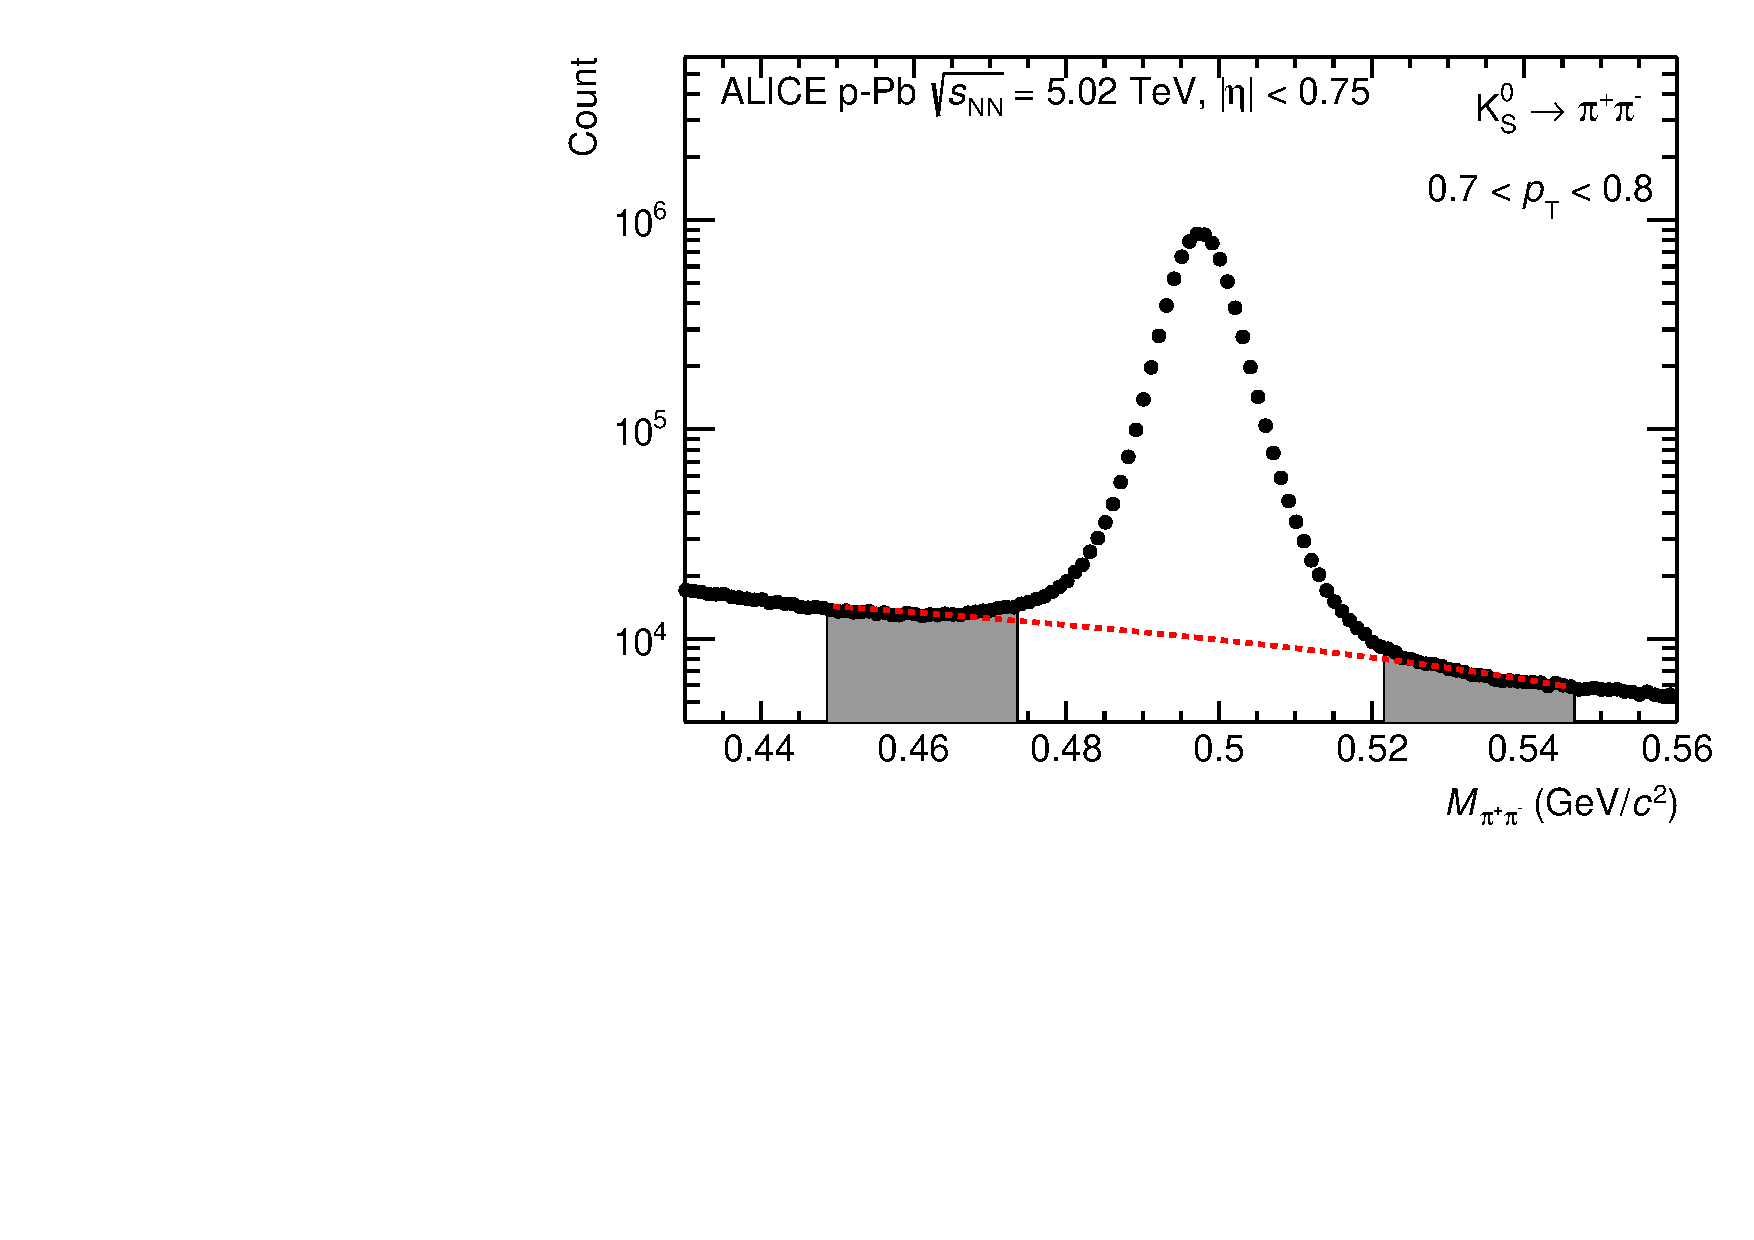
\includegraphics[width=.4\textwidth]{cf01_1}
		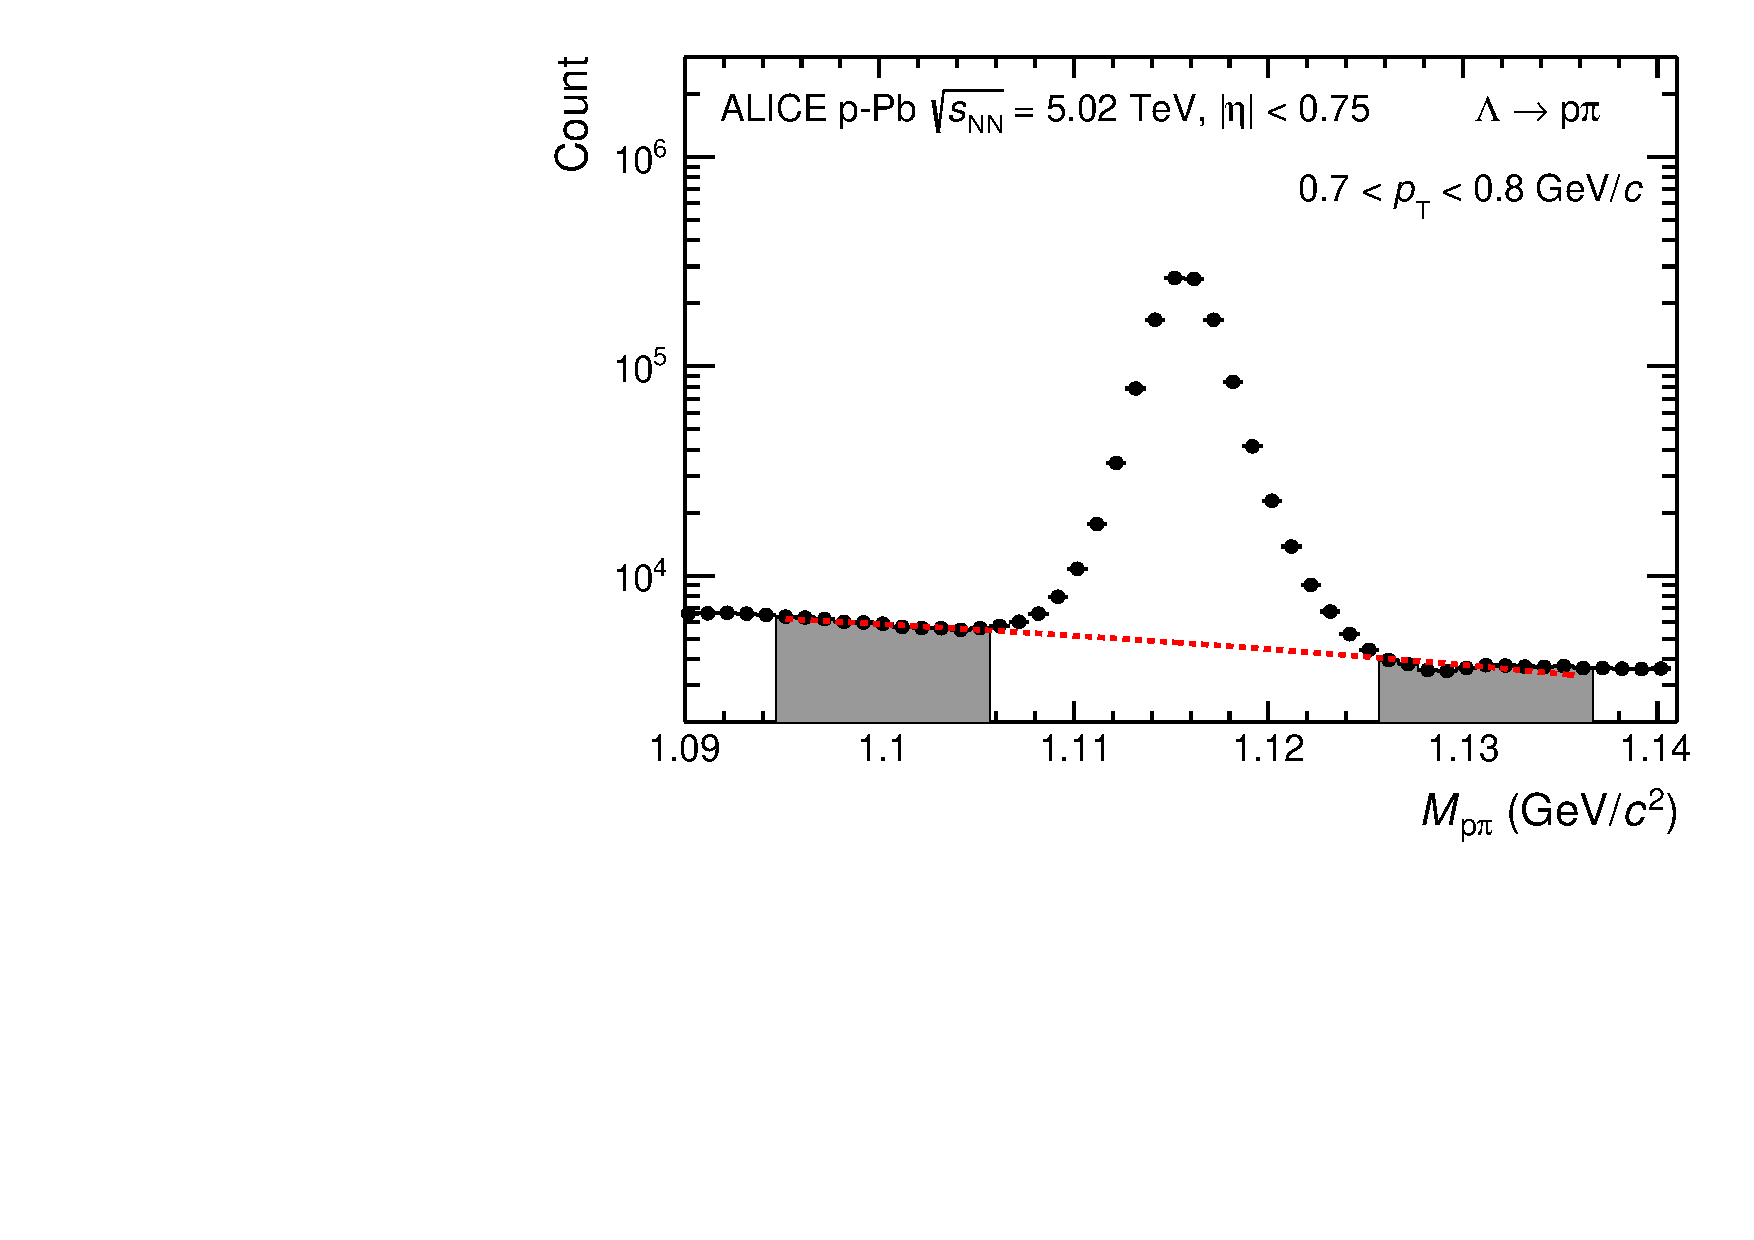
\includegraphics[width=.4\textwidth]{cf01_2}
		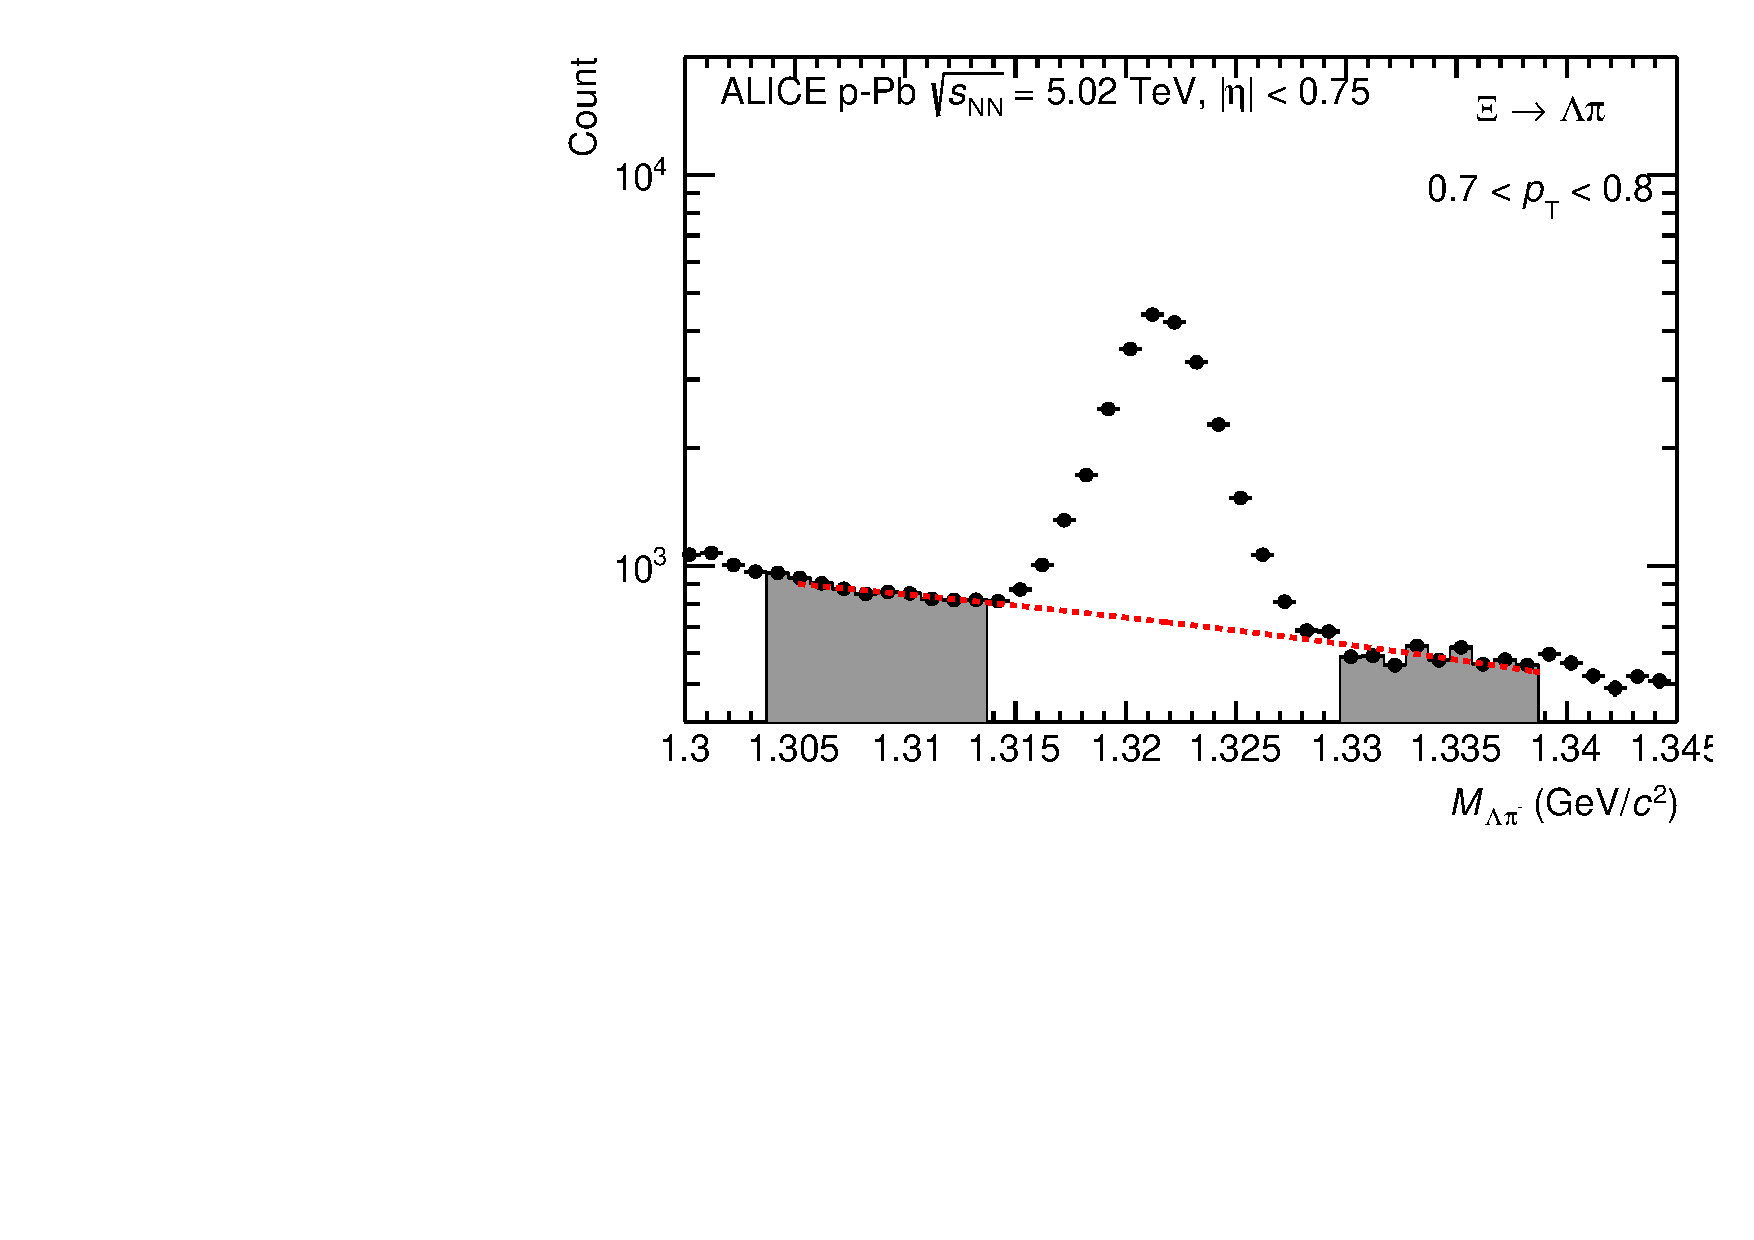
\includegraphics[width=.4\textwidth]{cf01_3}
		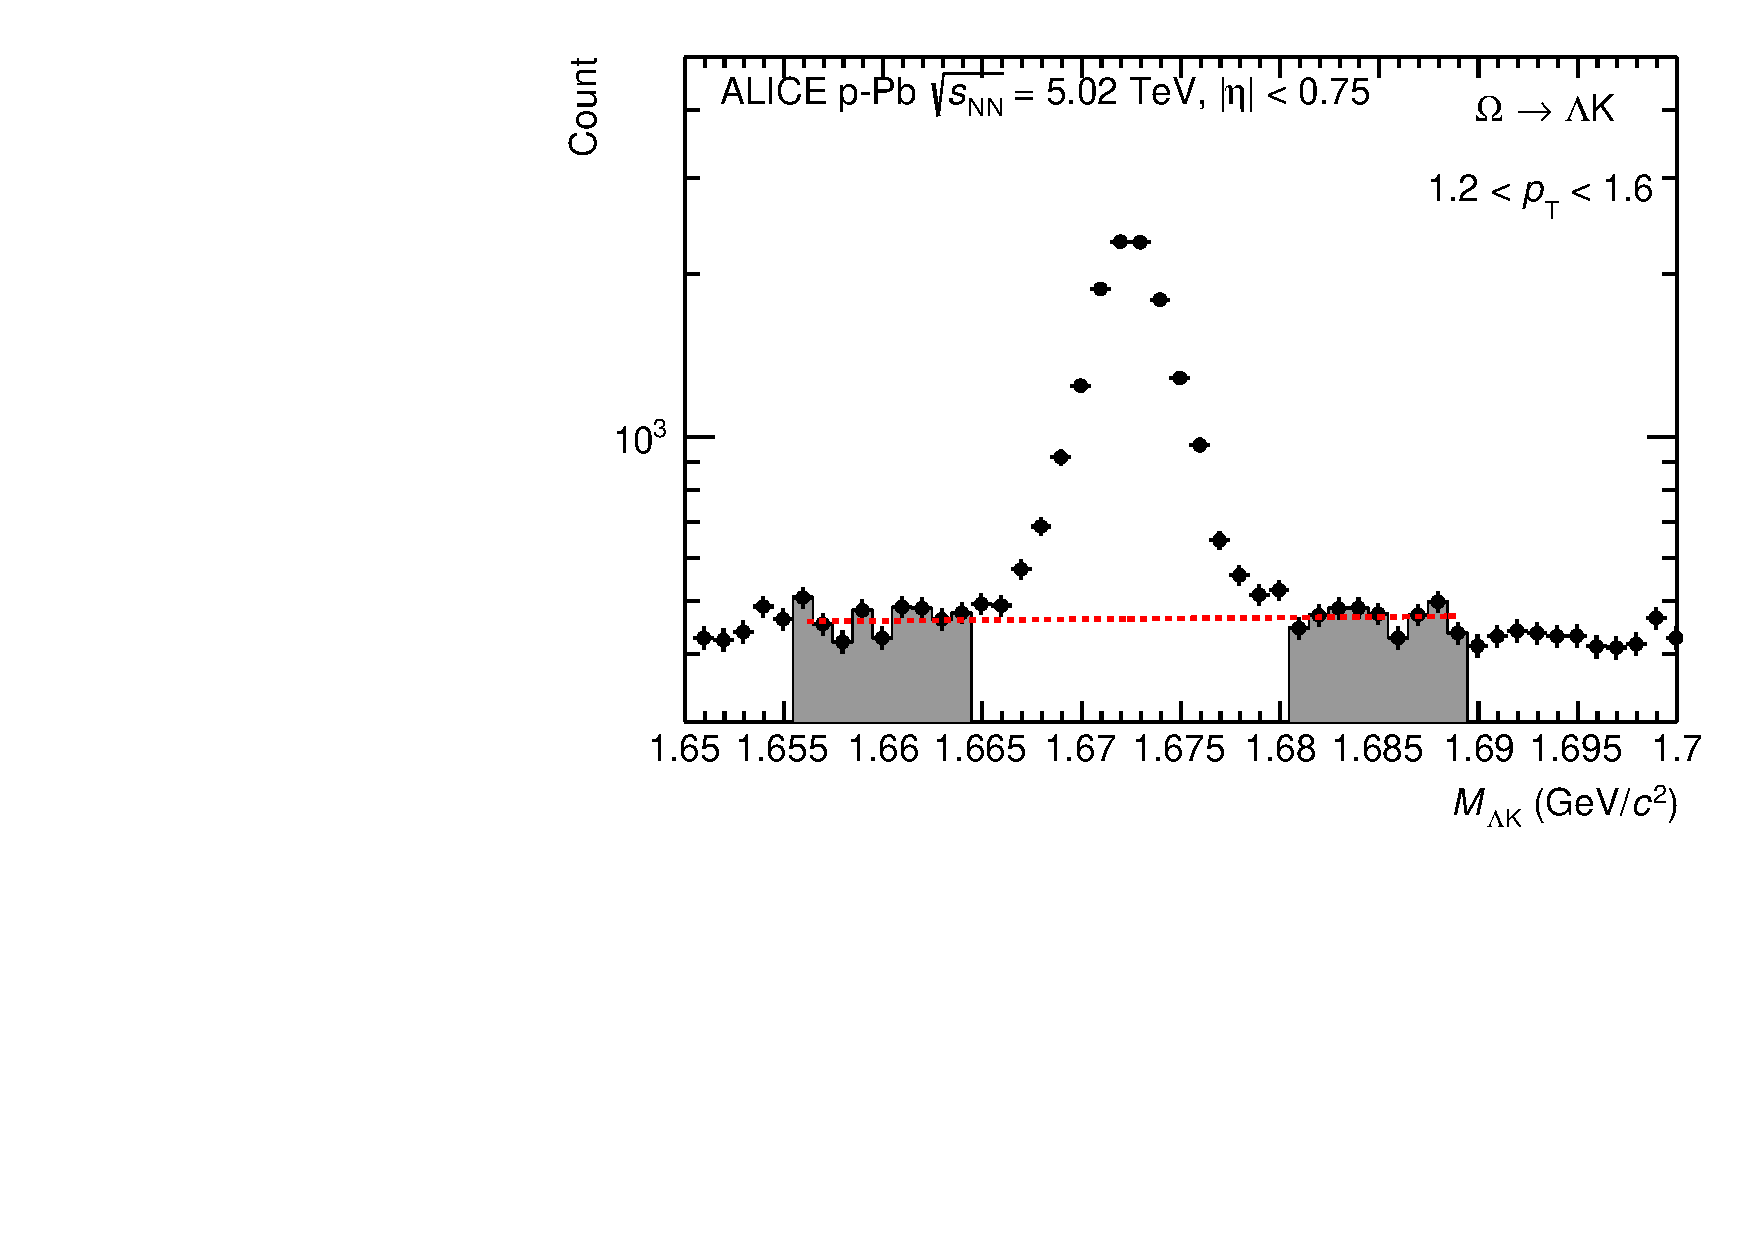
\includegraphics[width=.4\textwidth]{cf01_4}
		\caption{Invariant Mass distribution for $\kzero$, $\lmb$, $\Xi$ and $\Omega$ in different $\pT$ intervals in MB \pPb system. The candidates are reconstructed in $|\eta|<0.75$.
			The grey areas are used for signal extraction in the bin counting procedure.
			The red dashed lines represent the fit to the background distributions and the interpolate to the ``peak'' region.}
		\label{fig:InvM}
	\end{center}
\end{figure}

\subsection{Matching of strange particles to jets and underlying event}%
\label{sec:ParJetMatch}

The strategy of matching the (multi-)strange particles with jets follow those presented in earlier work~\cite{V0injet}.
The matching is done on a geometrical basis which presented in Eq.~\ref{eq:DParJet}.
\begin{equation}
d(\mathrm{particle, jet}) = \sqrt{(\eta_\mathrm{particle} -\eta_{\rm jet})^{2} + (\varphi_\mathrm{particle} -\varphi_{\rm jet})^{2}}
\label{eq:DParJet}
\end{equation}
If the distance between the particle candidate and the jet ($d$) is smaller than the matching distance $D$ (= 0.4), the candidate is considered to be inside the jet cone (JC).
The raw yields in JC are not only composed of the hadron produced via jet fragmentation (write as JE), but also hadron from Underlying Event (UE), which is defined as the sum of all particles which are not produced via hard parton fragmentation.
The UE contribution is estimated by Perpendicular Cone (PC) yields.
The PC indicates the cone, which is located in $\eta \times \varphi$ space in the perpendicular direction to the jet axis at the same $\eta$.
The systematic uncertainty due to the UE subtraction is estimated by the particle in Outside jet Cone(OC) yields.

In addiction, the acceptance selections of inclusive (regardless of the association between particle and hard scattering), JC and UE (multi-)strange particles are different in the $\eta$--$\varphi$ plane.
To get the particle from JE the production yields are normalized to per-acceptance density ($\rho$).
\begin{equation}
\begin{split}
{\rm Inclusive:}\qquad & \frac{\dd\rho}{\dd\pT} = \frac{1}{N_{\rm ev}}\times\frac{1}{\Delta\eta\Delta\varphi}\times\frac{\dd N}{\dd\pT} \\
{\rm JC:}\qquad & \frac{\dd\rho}{\dd\pT} = \frac{1}{N_{\rm ev}^{\rm jet}} \times\frac{1}{\mathcal{P}_{\rm JC}\Delta\eta\Delta\varphi}\times\frac{\dd N}{\dd\pT} \\
{\rm PC:}\qquad & \frac{\dd\rho}{\dd\pT} = \frac{1}{N_{\rm ev}^{\rm jet}} \times\frac{1}{\mathcal{P}_{\rm PC}\Delta\eta\Delta\varphi}\times\frac{\dd N}{\dd\pT} \\
{\rm OC:}\qquad & \frac{\dd\rho}{\dd\pT} = \frac{1}{N_{\rm ev}^{\rm jet}} \times\frac{1}{\mathcal{P}_{\rm OC}\Delta\eta\Delta\varphi}\times\frac{\dd N}{\dd\pT} \\
\end{split}
\label{eq:normalize}
\end{equation}
where the $\mathcal{P}$ denotes the probability of particles in a given selection found in the $\eta$--$\varphi$ plane with respect to the inclusive one.

\subsection{Corrections for strange particles reconstruction and feed-down}
\label{SubSec:Correction}
The reconstruction efficiency of particles are obtained in Monte Carlo simulated data.
These are estimated using PYTHIA 8.2~\cite{Sjostrand:2014zea} and DPMJet~\cite{Roesler:2000he} generators in \pp and \pPb, respectively, and tracsported through a GEANT 3~\cite{Brun:1994aa}.
Due to different $\eta$-shape between particle in JC and the inclusive one, it is needed to take the $\eta$ dependence of different particle distributions into account~\cite{V0injet}.
Fig.~\ref{fig:EffiJCIncl} shows the difference of reconstruction efficiency of JC particles and the inclusive one.
\begin{figure}[!ht]
	\begin{center}
		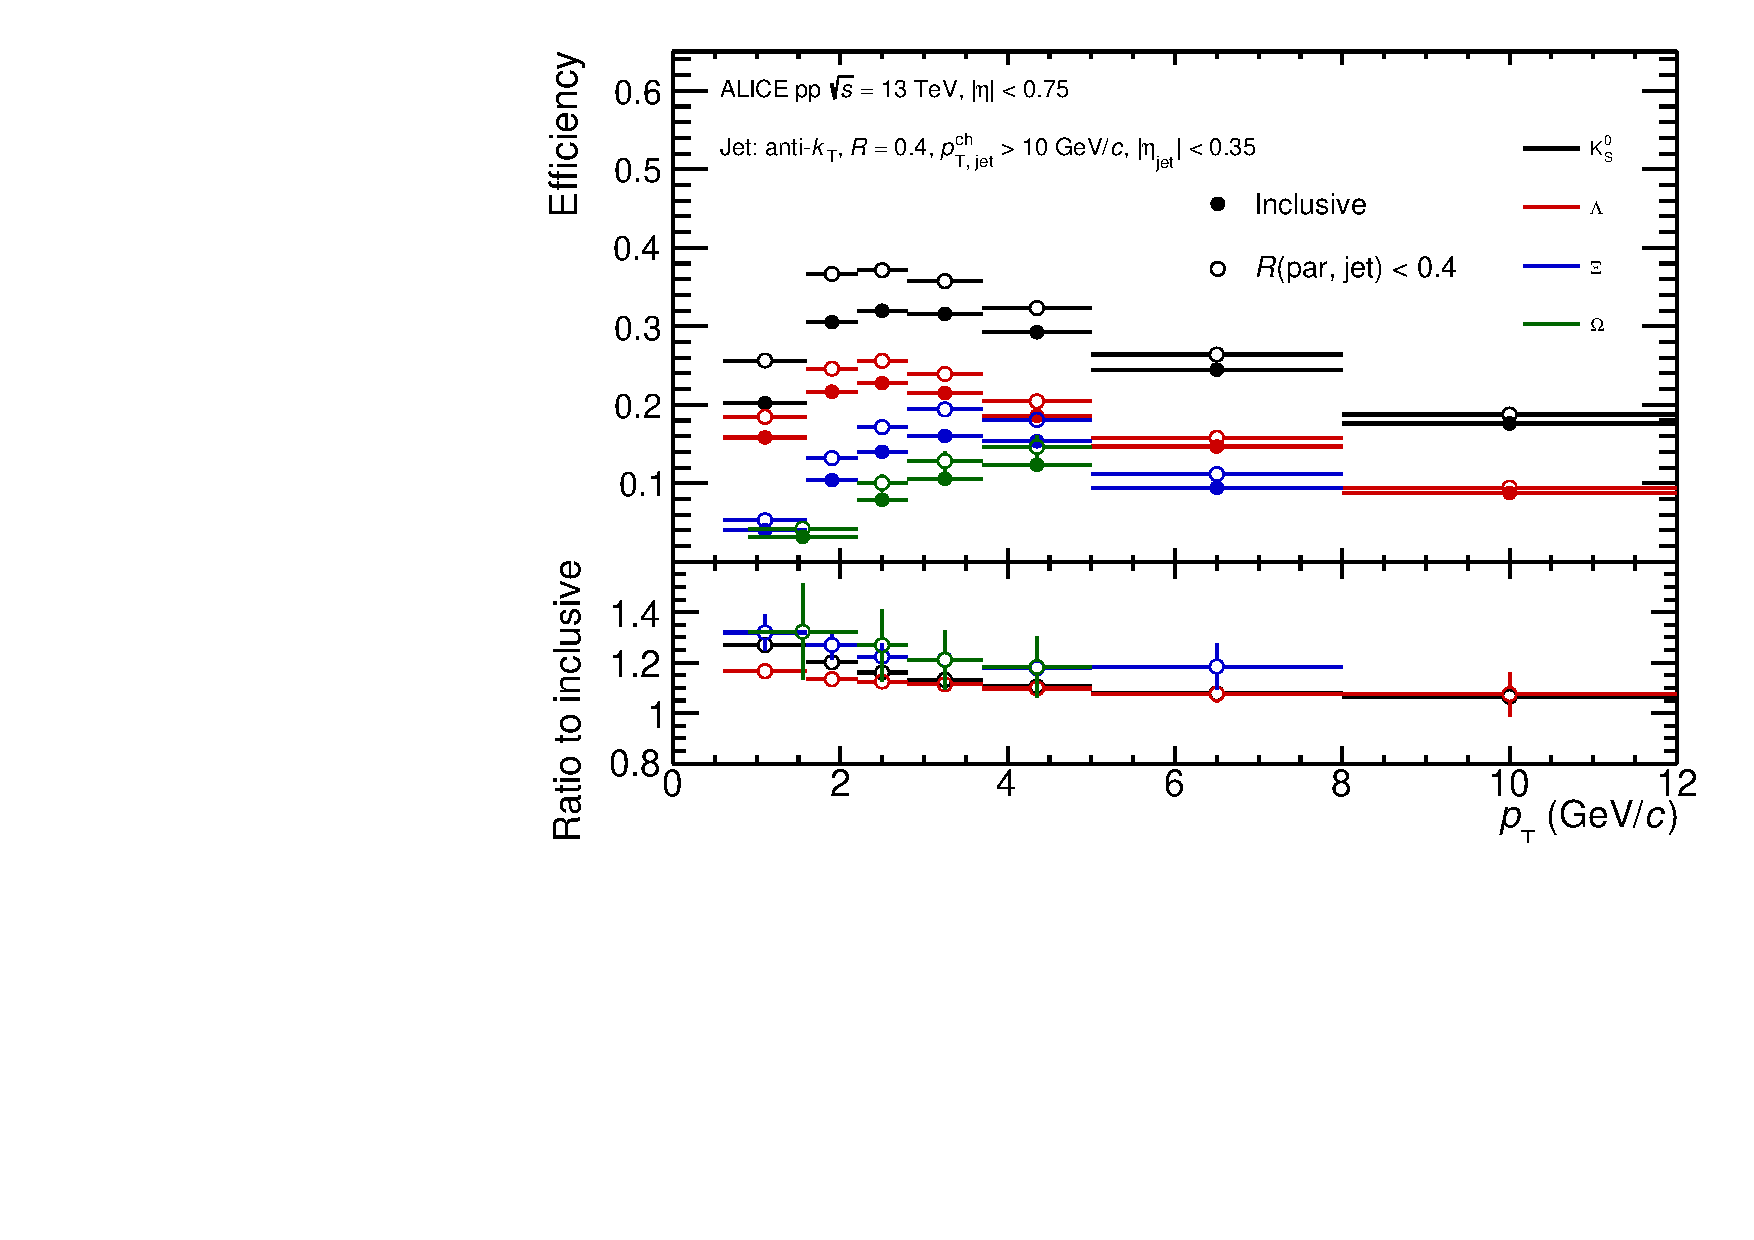
\includegraphics[width=.4\textwidth]{cf02_1}
		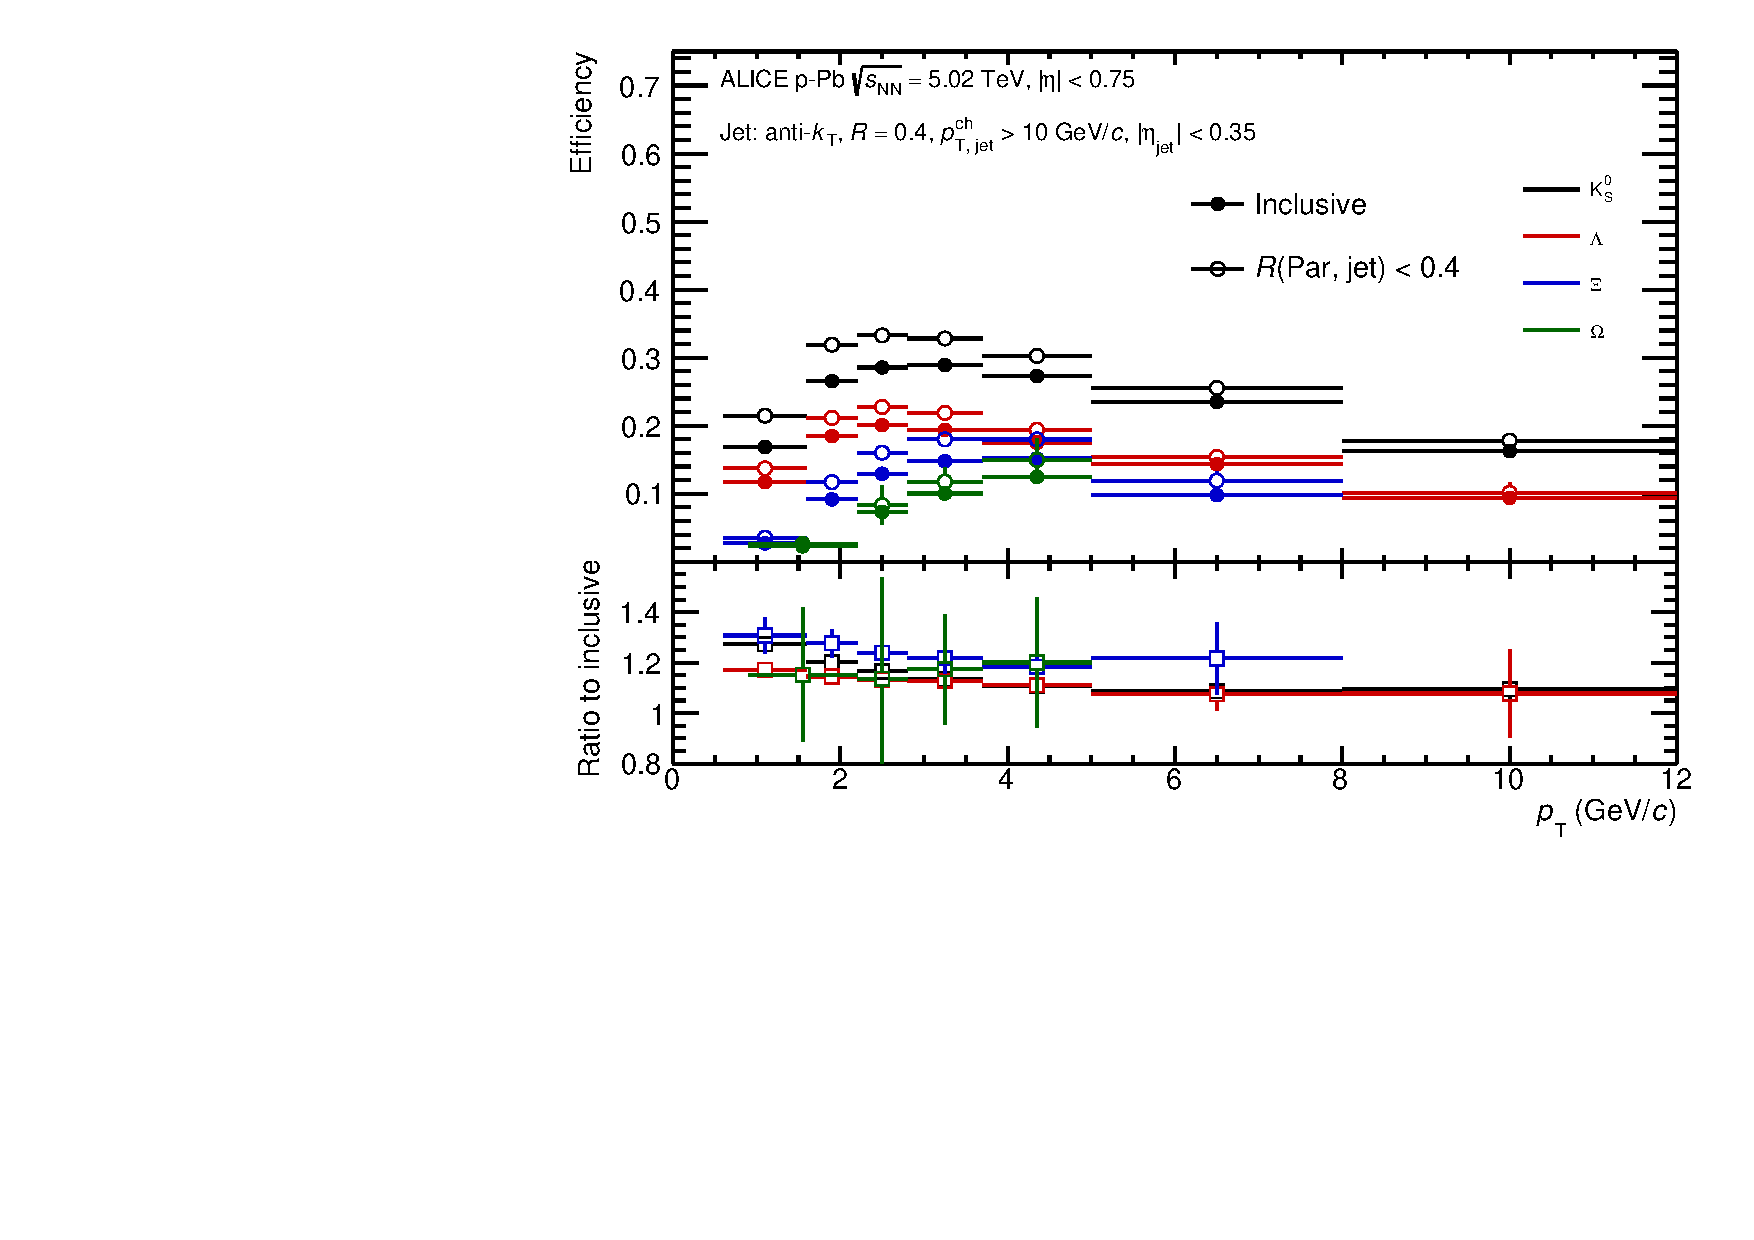
\includegraphics[width=.4\textwidth]{cf02_2}
	\end{center}
	\caption{The reconstruction efficiency for the particles in \pp collisions at \thirteen (left) and in \pPb collisions at \fivenn (right) for two selections: inside jet cone, $R(\mathrm{particle, jet}) < 0.4$ and the inclusive one.}
	\label{fig:EffiJCIncl}
\end{figure}

Only the yields for $\lmb$ and $\almb$ are significantly affected by secondary particles coming from the decays of charged and neutral $\Xi$ baryons.
The feed-down fraction is calculated with a data-driven approach~\cite{Abelev:2013haa}.
The detailed of inclusive feed-down method has been introduced in previous ALICE analysis works~\cite{Acharya:2019kyh, Acharya:2020uxl, ALICE:2017jyt}.
In particular, the $\lmb$ and $\almb$ in jet and UE feed-down component usually estimated by inclusive $\Xis$ spectra and PYTHIA simulations~\cite{V0injet}, due to lack of $\Xis$ in jet and UE results.
In this work, the feed-down fraction in jets and UE is computed for each $\pT$ bin by the measured $\Xis$ in jets and UE spectra, thereby assuming that the production rates of charged and neutral $\Xi$ are equal.
Figure~\ref{fig:FdFrac} shows the results of feed-down fraction in JC and the inclusive one.
\begin{figure}[!ht]
	\begin{center}
		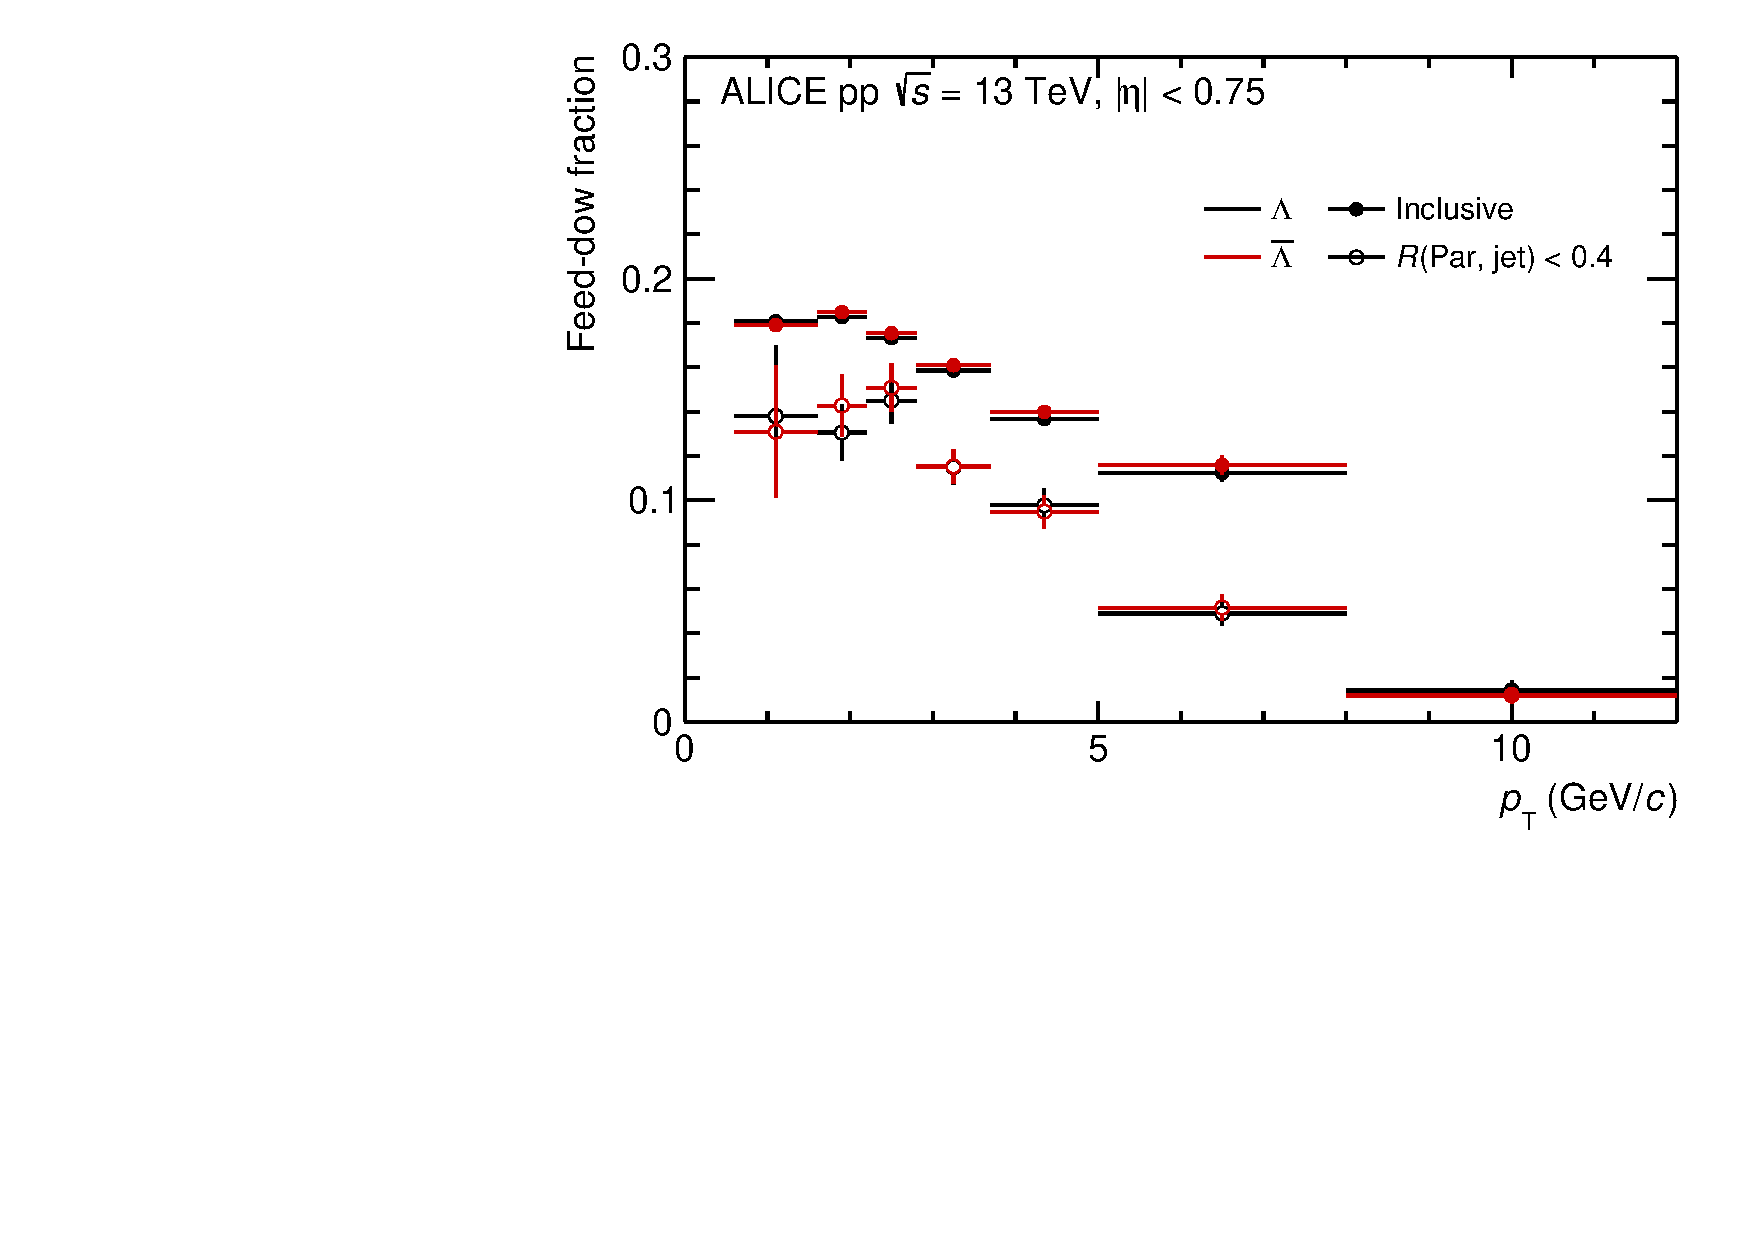
\includegraphics[width=.4\textwidth]{cf03_1}
		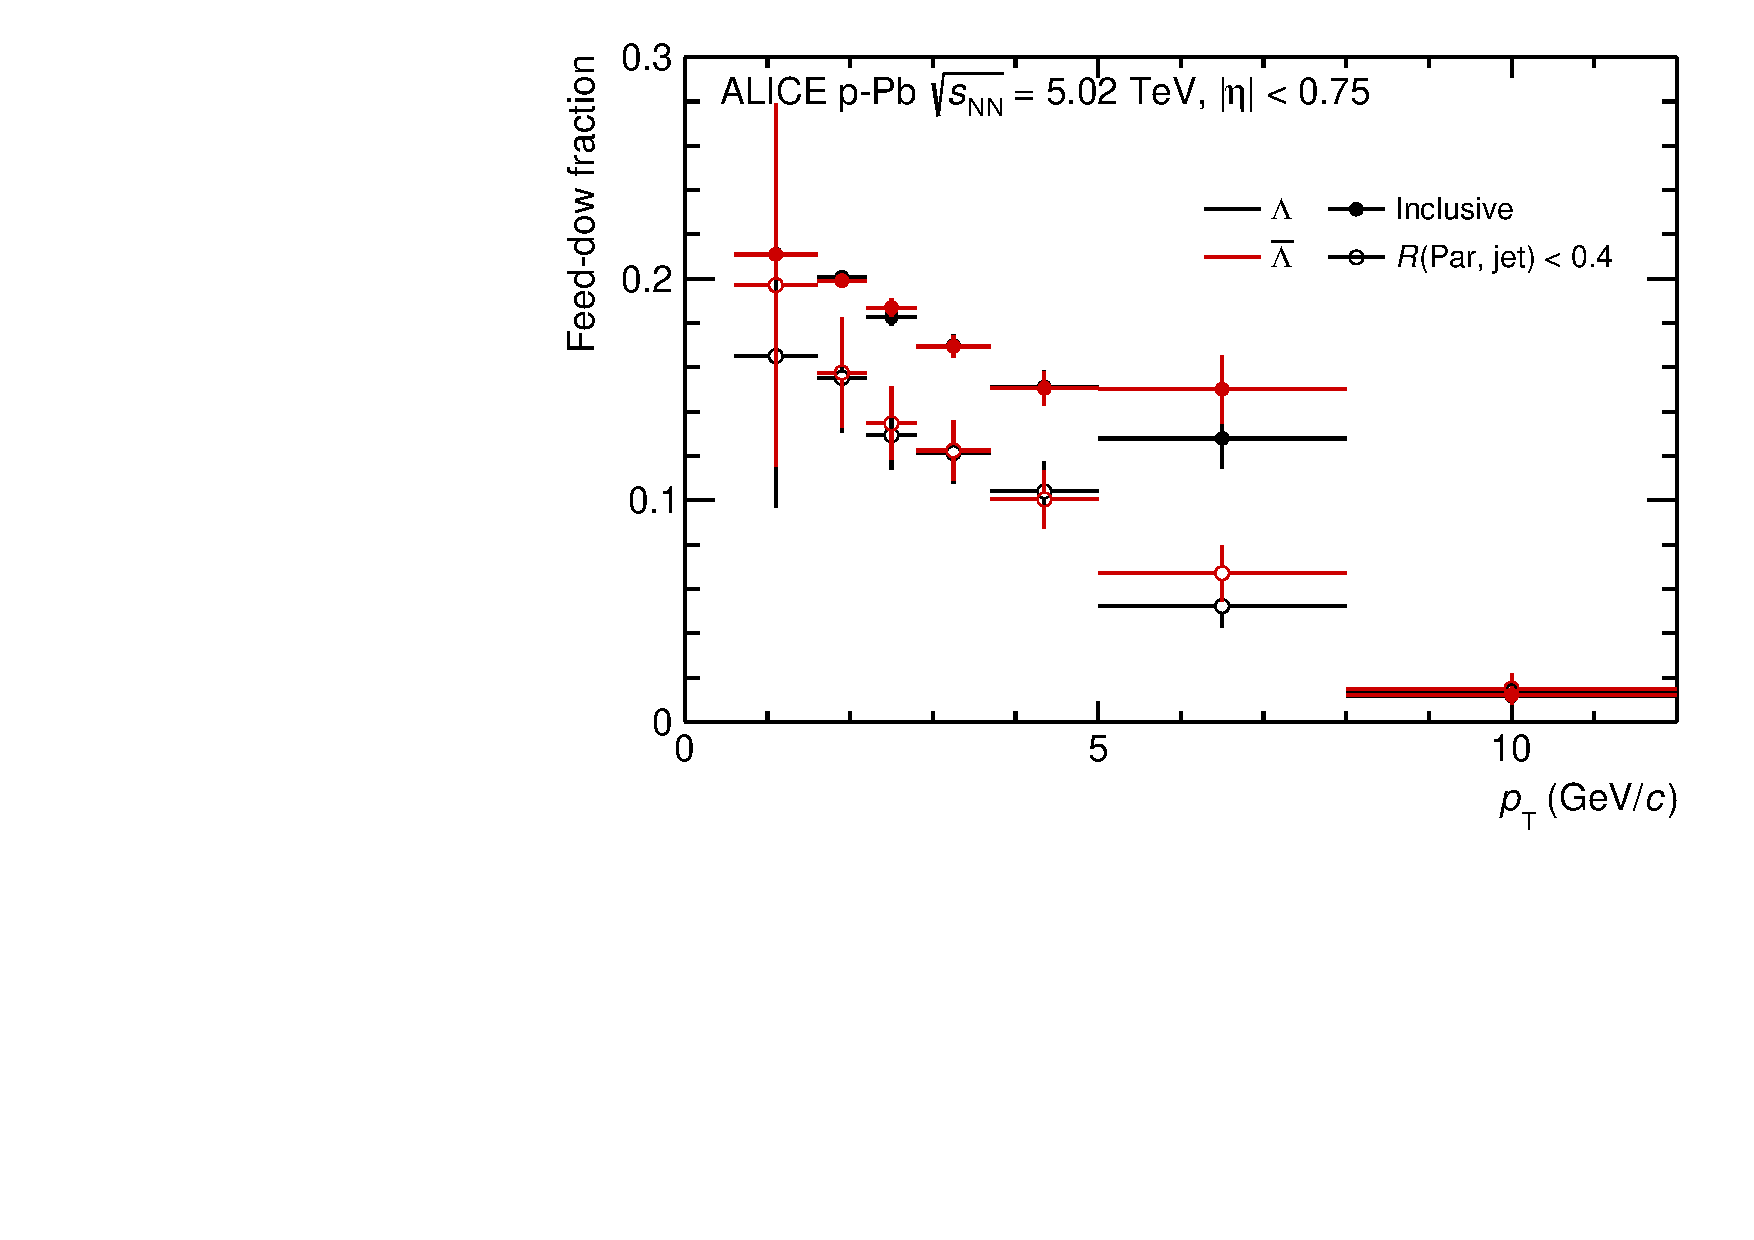
\includegraphics[width=.4\textwidth]{cf03_2}
	\end{center}
	\caption{Fraction of $\lmb$ spectra removed due to feed-down subtraction of charged and neutral $\Xi$}
	\label{fig:FdFrac}
\end{figure}

\subsection{Systematic uncertainties}
\label{sec:SysUncer}
The total systematic uncertainty, for $\kzero$, $\lmb$, $\almb$, $\Xis$ and $\Oms$ reconstruction of each data point of the final results, due to the choice of selection criteria are estimated separately in each $\pT$ interval.
Individual settings are loosened and tightened, in order to measure changes in the signal loss correction.
The main sources of the systematic uncertainty in this measurements are knowledge of detector materials, track selections, particle identification, proper lifetime, topological selection and signal extraction.
All these individual error contributions, which are listed in Tab.~\ref{tab:ppInclUncer}, \ref{tab:pPbInclUncer} are added in quadrature.
\begin{table}[!ht]
	\begin{center}
		\caption{Main sources and values of the relative systematic uncertainties(\%) of $\kzero$, $\lmb + \almb$, $\X + \Ix$ and $\Om + \Mo$ in \pp collisions at \thirteen.
			The value are reported for low, intermediate and high $\pT$.}
		\label{tab:ppInclUncer}
		\begin{tabularx}{\textwidth}{@{} lCCCCCCCCCCCC @{}}
			\toprule
			\textbf{Uncertainty source} & \multicolumn{3}{c}{\textbf{$\kzero$}}
			& \multicolumn{3}{c}{\textbf{$\lmb + \almb$}}
			& \multicolumn{3}{c}{\textbf{$\X + \Ix$}}
			& \multicolumn{3}{c}{\textbf{$\Om + \Mo$}} \\
			\cmidrule(lr){2-4} \cmidrule(lr){5-7} \cmidrule(lr){8-10} \cmidrule(lr){11-13}
			$\pT$ (\GeVc)    & 0.6 & 2 &10  & 0.6 & 2 & 10  & 0.6 & 2 & 7   & 1& 2 & 5 \\
			\midrule
			Detector material & 4 & 4 & 4 & 4 & 4 & 4 & 4 & 4 & 4 & 4 & 4 & 4 \\
			Track selection &  1.5 & 1.2 & 0.4 & 0.6 & 1.4 & 1.3 & 2.8 & 0.1 & 0. & 0. & 1.5 & 0.2\\
			Particle identification& 0.1& 0.1& 0.1 & 0.3 & 0.2 & 1.1 & 1.9 & 1.7 & 2.4& 3.9& 8.7& 6.\\
			Proper lifetime& 0& 0.1& 0& 2.1& 0.4& 0& -& -& -& -& -& -\\
			Topological& 0.2& 1.4& 0& 3.9& 0.8& 3.9& 0.6& 0.9& 1.& 2.8& 5.4& 2.4\\
			Signal extraction& 0.8& 1.1& 1.1& 0.3& 0.5& 1.7& 3. & 1.& 0.5& 2.3& 4.6& 3 \\
			\midrule
			\textbf{Total uncertainty}& 4.4& 4.6& 4.2& 6.1& 4.4& 6.1& 6.1& 4.5& 4.8& 6.7& 12.& 8.2\\
			\bottomrule
		\end{tabularx}
	\end{center}
\end{table}

\begin{table}[!ht]
	\begin{center}
		\caption{Main sources and values of the relative systematic uncertainties(\%) of $\kzero$, $\lmb + \almb$, $\X + \Ix$ and $\Om + \Mo$ in \pPb collisions at \fivenn.
			The value are reported for low, intermediate and high $\pT$.}
		\label{tab:pPbInclUncer}
		\begin{tabularx}{\textwidth}{@{} lCCCCCCCCCCCC @{}}
			\toprule
			\textbf{Uncertainty source} & \multicolumn{3}{c}{\textbf{\kzero}}
			& \multicolumn{3}{c}{\textbf{$\lmb + \almb$}}
			& \multicolumn{3}{c}{\textbf{$\X + \Ix$}}
			& \multicolumn{3}{c}{\textbf{$\Om + \Mo$}} \\
			\cmidrule(lr){2-4} \cmidrule(lr){5-7} \cmidrule(lr){8-10} \cmidrule(lr){11-13}
			$\pT$ (\GeVc) & 0.6 & 2 &10  & 0.6 & 2 & 10    & 0.6 & 2 & 7   & 1& 2 & 5 \\
			\midrule
			Detector material& 0.4 & 0.4 & 0.4 & 0.4 & 0.4 & 0.4 & 0.4 & 0.4 & 0.4 & 0.4 & 0.4 & 0.4 \\
			Track selection & 1.4& 1.7& 1.8& 0.2& 1.3& 1.4& 0& 0& 0& 1.3& 2.5& 0\\
			Particle identification& 0.1& 0.2& 0.2& 0.3& 0.2& 1& 3.1&  1.2& 0& 8.1& 13.7& 5.9 \\
			Proper lifetime & 0& 0& 0& 1.6& 0.3& 0& 0.6& 0.4& 0& 0& 3.3& 0\\
			Topological & 4.4& 0.6& 1.9& 3.9& 0.9& 2.7& 1.3& 0& 2.6& 1.2& 4.8& 3.7\\
			Signal extraction& 0.3& 2.6& 1.7& 0.6& 0.5& 2.6& 5.1& 0.9& 2.6& 0& 5.2& 0\\
			\midrule
			\textbf{Total uncertainty}& 6.1& 5.1& 5.1& 5.8& 4.3& 5.8& 7.4& 4.3& 5.4& 9.2& 16.4& 8\\
			\bottomrule
		\end{tabularx}
	\end{center}
\end{table}

\textbf{Material budget.} The effect of the incomplete knowledge of the detector's material budget is evaluated by comparing different Monte Carlo simulations in which the material budget was increased and decreased by $4.5\%$.
This value corresponds to the uncertainty on the determination of the material budget by measuring photon conversions.
This particular systematic uncertainty is around $0.4\%$.

\textbf{Track selection.} To estimate the systematic due to the track selection, the analysis has been redone with the increased number of required clusters in the TPC.

\textbf{Particle identification.} The TPC $\dEdx$ selection is used to reduce the combinatorial background in the (multi-)strange particle invariant mass distribution.
The number of $\sigma$ in the identification of particles using the $\dEdx$ have been varied between $4\sigma$ to $6\sigma$.

\textbf{Proper lifetime selection.} The proper lifetime defied as $mLc/p$, which $m$ is the mass of particles, $L$ is the decay length, and $p$ is the particle's momentum.
The selection on the $mLc/p$ is varied from around $12$ to $40$~cm for $\kzero$, $20$ to $40$ cm for $\lmb$ $(\almb)$ and $2c\tau$ to $6c\tau$ for $\Xis$ and $\Oms$.

\textbf{Topological selection.} The values of the selection criteria on the topological variables are varied around their nominal values.
The observed deviations for each component are summed in quadrature.

\textbf{Signal extraction.} In the same spirit, the signal extraction technique has been tested by varying the widths used to define the ``signal" and ``background'' regions, expressed in terms of the number of $\sigma$ as defined in Sec.~\ref{sec:ParRec}.

The additional systematic uncertainty sources associated with particle yield in jet are originated from the UE subtraction estimator and the jet $\pT$ threshold.
In Sec.~\ref{sec:ParJetMatch}, it introduced two UE estimators, the PC and OC.
From the deviation of OC and PC, the relative systematic uncertainty of the UE subtraction is obtained.
To estimate the effect of jet $\pT$ thresholds uncertainty, the analysis is repeated with the jet $\pT$ cut $10\pm 1$~\GeVc.
The systematic of the particle in jets are added to the list of uncertainties in quadrature.
The value are shown in Table~\ref{tab:ppJEUncer}, \ref{tab:pPbJEUncer}.

\begin{table}[!ht]
	\begin{center}
		\caption{Main sources and values of the relative systematic uncertainties(\%) of $\kzero$, $\lmb + \almb$, $\X + \Ix$ and $\Om + \Mo$ in JE in \pp collisions at \thirteen.
			The value are reported for low, intermediate and high $\pT$.}
		\label{tab:ppJEUncer}
		\begin{tabularx}{\textwidth}{@{} lCCCCCCCCCCCC @{}}
			\toprule
			\textbf{Uncertainty source} & \multicolumn{3}{c}{\textbf{\kzero}}
			& \multicolumn{3}{c}{\textbf{$\lmb + \almb$}}
			& \multicolumn{3}{c}{\textbf{$\X + \Ix$}}
			& \multicolumn{3}{c}{\textbf{$\Om + \Mo$}} \\
			\cmidrule(lr){2-4} \cmidrule(lr){5-7} \cmidrule(lr){8-10} \cmidrule(lr){11-13}
			$\pT$ (\GeVc) & 0.6 & 2 &10  & 0.6 & 2 & 10    & 0.6 & 2 & 7   & 1& 2 & 5 \\
			\midrule
			Particle reconstruction& 1.8& 0.25& 0.1& 5.3& 0.6& 0& 6.7& 0.9& 0.1& 6& 1.7& 0.3\\
			UE subtraction& 0.1& 0.1& 0.1& 0.1& 0.2& 0.1& 1.5& 0.2& 0.3& 3.6& 1.8& 0.5\\
			Jet $\pT$ threshold& 0.6& 3,1& 10.9& 0.6& 1.1& 9.9& 3.5& 2.4& 5& 0& 0& 0\\
			\midrule
			\textbf{Total uncertainty}& 1.8& 3.1& 10.9& 5.3& 1.2& 9.9& 7.7& 2.6& 5& 7.1& 2.5& 0.6 \\
			\bottomrule
		\end{tabularx}
	\end{center}
\end{table}

\begin{table}[!ht]
	\begin{center}
		\caption{Main sources and values of the relative systematic uncertainties(\%) of $\kzero$, $\lmb + \almb$, $\X + \Ix$ and $\Om + \Mo$ in JE in \pPb collisions at \fivenn.
			The value are reported for low, intermediate and high $\pT$.}
		\label{tab:pPbJEUncer}
		\begin{tabularx}{\textwidth}{@{} lCCCCCCCCCCCC @{}}
			\toprule
			\textbf{Uncertainty source} & \multicolumn{3}{c}{\textbf{\kzero}}
			& \multicolumn{3}{c}{\textbf{$\lmb + \almb$}}
			& \multicolumn{3}{c}{\textbf{$\X + \Ix$}}
			& \multicolumn{3}{c}{\textbf{$\Om + \Mo$}} \\
			\cmidrule(lr){2-4} \cmidrule(lr){5-7} \cmidrule(lr){8-10} \cmidrule(lr){11-13}
			$\pT$ (\GeVc) & 0.6 & 2 &10  & 0.6 & 2 & 10    & 0.6 & 2 & 7   & 1& 2 & 5 \\
			\midrule
			Particle reconstruction& 5& 0.8& 0& 13.2& 1.5& 0& 24.8& 2.8& 0.3& 8.7& 3.7& 0.9\\
			UE subtraction& 0.3& 0.1& 0.1& 0& 0.1& 11.2& 14.1& 0.8& 0.7& 0& 0& 1.2\\
			Jet $\pT$ threshold& 0.3& 3.5& 11& 3.2& 1.8& 0.1& 24.9&  3& 4.1& 3.1& 10.7& 7.6\\
			\midrule
			\textbf{Total uncertainty}& 5& 3.6& 11& 13.5& 2.3& 11.2& 37.9& 4.2& 4.1& 9.3& 11.3& 7.7 \\
			\bottomrule
		\end{tabularx}
	\end{center}
\end{table}

The uncertainty of jet cone particle ratios ($\lmb/\kzero$, $\Xi/\kzero$, $\Omega/\kzero$, $\Xi/\lmb$, $\Omega/\lmb$ and $\Omega/\Xi$) also consider three sources: the particle reconstruction, UE subtraction and the jet $\pT$ threshold.
The particle reconstruction uncertainty is propagated from the spectra.
Uncertainties related to UE subtraction and jet $\pT$ threshold are obtained by varying the condition in both numerator and denominator of the corresponding ratios.

\begin{table}[!ht]
	\begin{center}
		\caption{Main sources and values of the relative systematic uncertainties(\%) of baryon-to-meson ratios ($\lmb/\kzero$, $\Xi/\kzero$, $\Omega/\kzero$) in JE in \pp collisions at \thirteen.
			The value are reported for low, intermediate and high $\pT$.}
		\label{tab:ppBMRatioUncer}
		\begin{tabularx}{\textwidth}{@{} lCCCCCCCCC @{}}
			\toprule
			\textbf{Uncertainty source} & \multicolumn{3}{c}{\textbf{$(\lmb + \almb)/(2\kzero)$}}
			& \multicolumn{3}{c}{\textbf{$(\X + \Ix)/(2\kzero)$}}
			& \multicolumn{3}{c}{\textbf{$(\Om + \Mo)/(2\kzero)$}} \\
			\cmidrule(lr){2-4} \cmidrule(lr){5-7} \cmidrule(lr){8-10}
			$\pT$ (\GeVc) & 0.6 & 2 &10  & 0.6 & 2 & 7 & 1 & 2 & 5 \\
			\midrule
			Particle reconstruction& 2.4& 2.8& 2.5& 3.4& 2.8& 2.8& 6.7& 11.4& 7.3\\
			UE subtraction& 0.8& 0.2& 0.4& 3.5& 0.2& 0.1& 10& 4& 2.2\\
			Jet $\pT$ threshold& 0.4& 2.3& 1& 1.7& 1.6& 3.6& 1.& 3.3& 6.4\\
			\midrule
			\textbf{Total uncertainty}& 2.6& 3.7& 2.7& 5.2& 3.3& 4.5& 12.4& 12.5& 10\\
			\bottomrule
		\end{tabularx}
	\end{center}
\end{table}

\begin{table}[!ht]
	\begin{center}
		\caption{Main sources and values of the relative systematic uncertainties(\%) of baryon-to-baryon ratios ($\Xi/\lmb$, $\Omega/\lmb$, $\Omega/\Xi$) in JE in \pp collisions at \thirteen.
			The value are reported for low, intermediate and high $\pT$.}
		\label{tab:ppBBRatioUncer}
		\begin{tabularx}{\textwidth}{@{} lCCCCCCCCC @{}}
			\toprule
			\textbf{Uncertainty source} & \multicolumn{3}{c}{\textbf{$(\X + \Ix)/(\lmb + \almb)$}}
			& \multicolumn{3}{c}{\textbf{$(\Om + \Mo)/(\lmb + \almb)$}}
			& \multicolumn{3}{c}{\textbf{$(\Om + \Mo)/(\X + \Ix)$}} \\
			\cmidrule(lr){2-4} \cmidrule(lr){5-7} \cmidrule(lr){8-10}
			$\pT$ (\GeVc) & 0.6 & 2 &7  & 1 & 2 & 5 & 1 & 2 & 5 \\
			\midrule
			Particle reconstruction& 3.4& 3& 3.2& 6.7& 11.5& 7.5& 6.8& 11.5& 7.4\\
			UE subtraction& 4.4& 0.4& 0.2& 12.4& 4.2& 2.3& 7.8& 3.8& 2.7\\
			Jet $\pT$ threshold& 0.7& 0.5& 1.9& 0.2& 0.9& 3.5& 0.4& 1.3& 3\\
			\midrule
			\textbf{Total uncertainty}& 5.6& 3& 3.7& 14.1& 12.2& 8.6& 10.3& 12.1& 8.5\\
			\bottomrule
		\end{tabularx}
	\end{center}
\end{table}

\begin{table}[!ht]
	\begin{center}
		\caption{Main sources and values of the relative systematic uncertainties(\%) of baryon-to-meson ratios ($\lmb/\kzero$, $\Xi/\kzero$, $\Omega/\kzero$) in JE in \pPb collisions at \fivenn.
			The value are reported for low, intermediate and high $\pT$.}
		\label{tab:pPbBMRatioUncer}
		\begin{tabularx}{\textwidth}{@{} lCCCCCCCCC @{}}
			\toprule
			\textbf{Uncertainty source} & \multicolumn{3}{c}{\textbf{$(\lmb + \almb)/(2\kzero)$}}
			& \multicolumn{3}{c}{\textbf{$(\X + \Ix)/(2\kzero)$}}
			& \multicolumn{3}{c}{\textbf{$(\Om + \Mo)/(2\kzero)$}} \\
			\cmidrule(lr){2-4} \cmidrule(lr){5-7} \cmidrule(lr){8-10}
			$\pT$ (\GeVc) & 0.6 & 2 &10  & 0.6 & 2 & 7 & 1 & 2 & 5 \\
			\midrule
			Particle reconstruction& 3.2& 3.4& 3.3& 4.7& 3.2& 4& 9.8& 1.5& 7.4\\
			UE subtraction& 0.8& 0.1& 0.1& 9.1& 1.8& 1& 4.1& 0& 0.3\\
			Jet $\pT$ threshold& 1.4& 2.6& 0.1& 8.6& 2.4& 6& 0.5& 1.5& 0.3\\
			\midrule
			\textbf{Total uncertainty}& 3.6& 4.3& 3.3& 13.4& 4.4& 7.2& 10.6& 15.1& 7.4\\
			\bottomrule
		\end{tabularx}
	\end{center}
\end{table}
\begin{table}[!ht]
	\begin{center}
		\caption{Main sources and values of the relative systematic uncertainties(\%) of baryon-to-baryon ratios ($\Xi/\lmb$, $\Omega/\lmb$, $\Omega/\Xi$) in JE in \pPb collisions at \fivenn.
			The value are reported for low, intermediate and high $\pT$.}
		\label{tab:pPbBBRatioUncer}
		\begin{tabularx}{\textwidth}{@{} lCCCCCCCCC @{}}
			\toprule
			\textbf{Uncertainty source} & \multicolumn{3}{c}{\textbf{$(\X + \Ix)/(\lmb + \almb)$}}
			& \multicolumn{3}{c}{\textbf{$(\Om + \Mo)/(\lmb + \almb)$}}
			& \multicolumn{3}{c}{\textbf{$(\Om + \Mo)/(\X + \Ix)$}} \\
			\cmidrule(lr){2-4} \cmidrule(lr){5-7} \cmidrule(lr){8-10}
			$\pT$ (\GeVc) & 0.6 & 2 &10  & 0.6 & 2 & 7 & 1 & 2 & 5 \\
			\midrule
			Particle reconstruction& 4.1& 2.8& 3.7& 9.6& 15& 7.5& 10& 14.9& 8.6\\
			UE subtraction& 9.9& 1.9& 0.8& 3.6& 0.1& 0.3& 11& 1.8& 0.1\\
			Jet $\pT$ threshold& 2.7& 0.6& 2.6& 0.4& 5& 3& 0.4& 3.8& 1.7\\
			\midrule
			\textbf{Total uncertainty}& 11.1& 3.4& 4.6& 10.3& 15.8& 8.1& 14.9& 15.5& 8.7\\
			\bottomrule
		\end{tabularx}
	\end{center}
\end{table}

\section{Results and discussion}%
\label{sec:Results}

\subsection{Particles $\pT$-differential density}
\label{subsec:ParPtDensity}

For the strange hadrons discussed in this paper, the ratios of yields for particles and anti-particles are around one within the uncertainties, as expected at these collision energies in the mid-rapidity region.
Therefore, all the $\pT$-differential density is shown in the following are reported after summing particles and anti-particles.
The different selections shown in the following have been introduced in section~\ref{sec:ParJetMatch}, inwhich also introduced the normalization method.

The $\pT$-differential density ($\dd \rho/ \dd \pT$ defined by Eq.~\ref{eq:normalize}), for all particle species, in \pp and MB \pPb collisions are shown in Fig.~\ref{fig:ppSpect} and \ref{fig:pPbSpect}, respectively.
All the hadrons' densities with $\pT$ are observed to become harder within events that require at least one charged particle jet with $\pTjch > 10$~\GeVc.
Also, as expected, the particle $\pT$-differential density in jet is harder than that in underlying events.

\begin{figure}[!ht]
	\begin{center}
		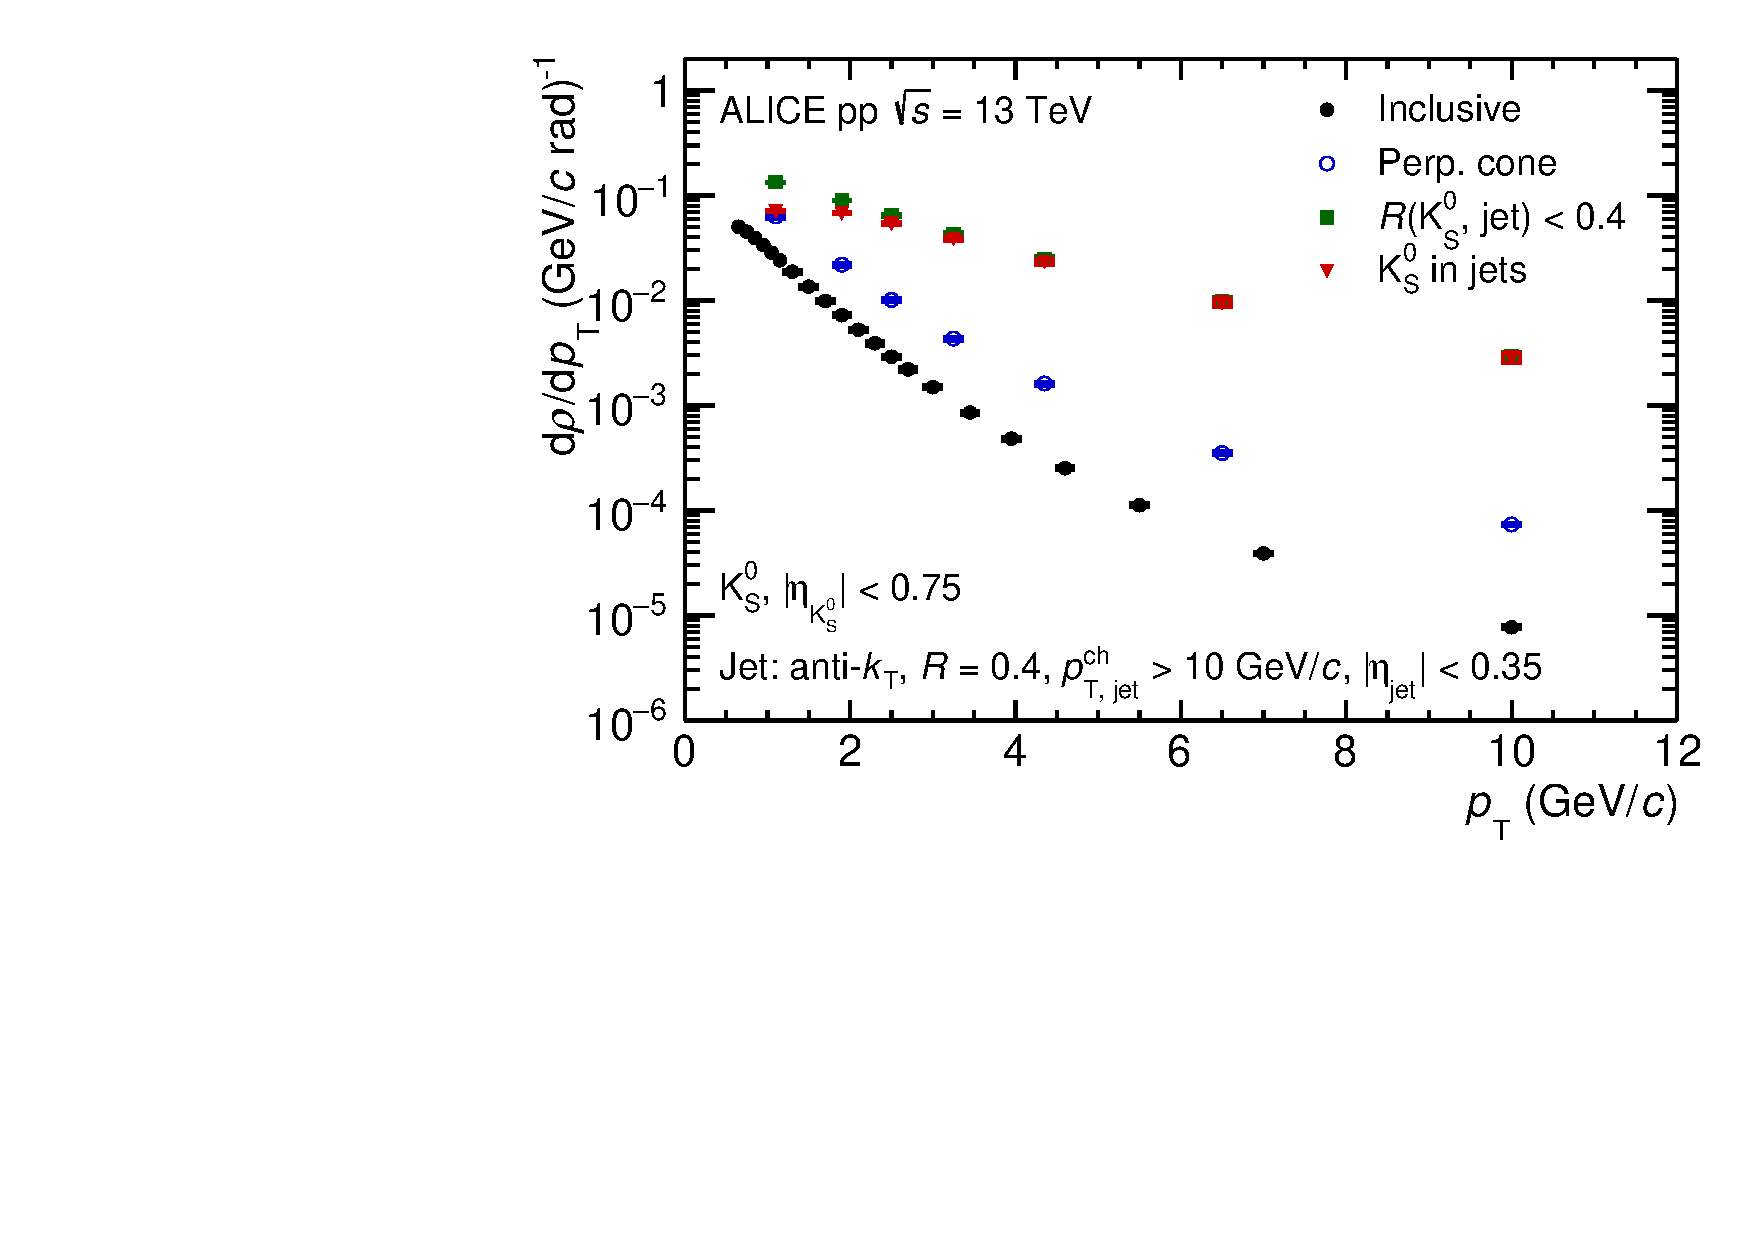
\includegraphics[width=.4\textwidth]{cf04_1}
		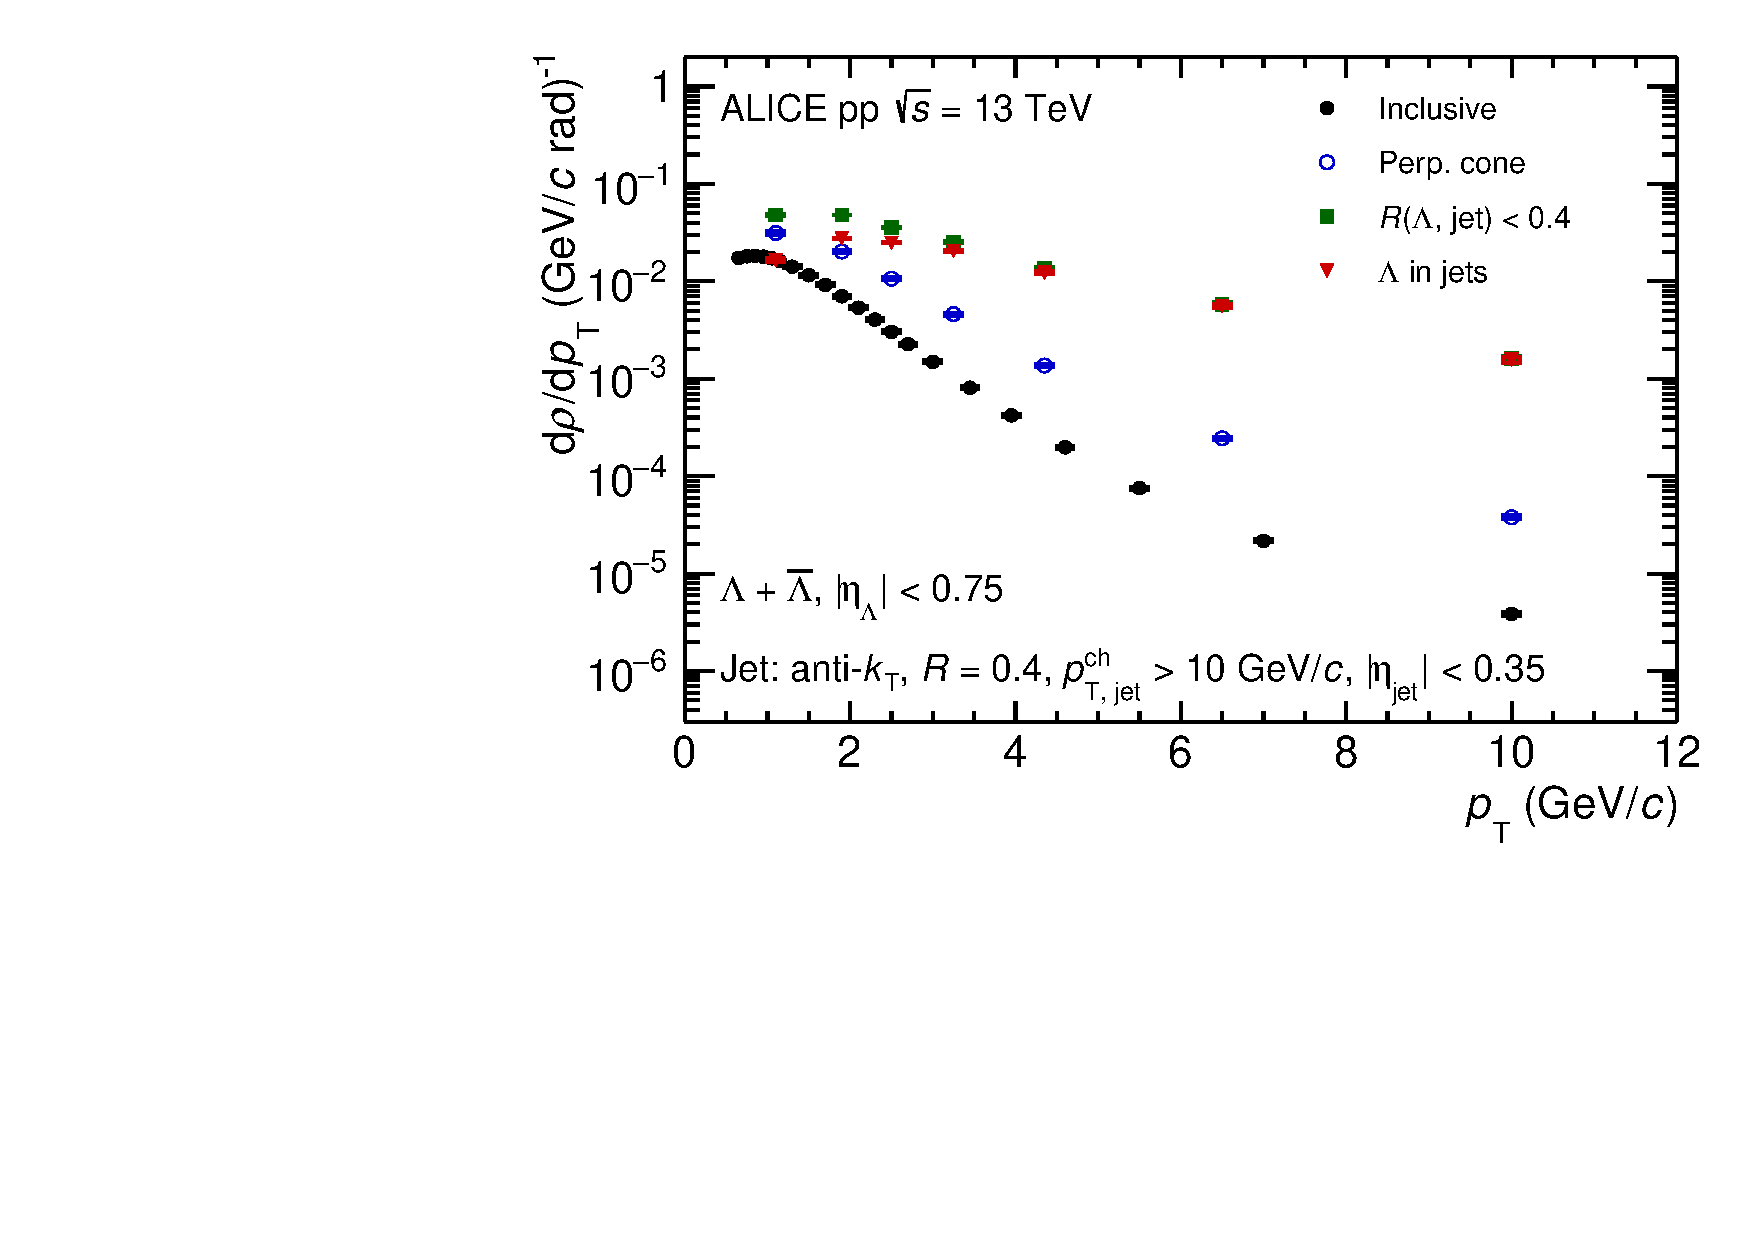
\includegraphics[width=.4\textwidth]{cf04_2}
		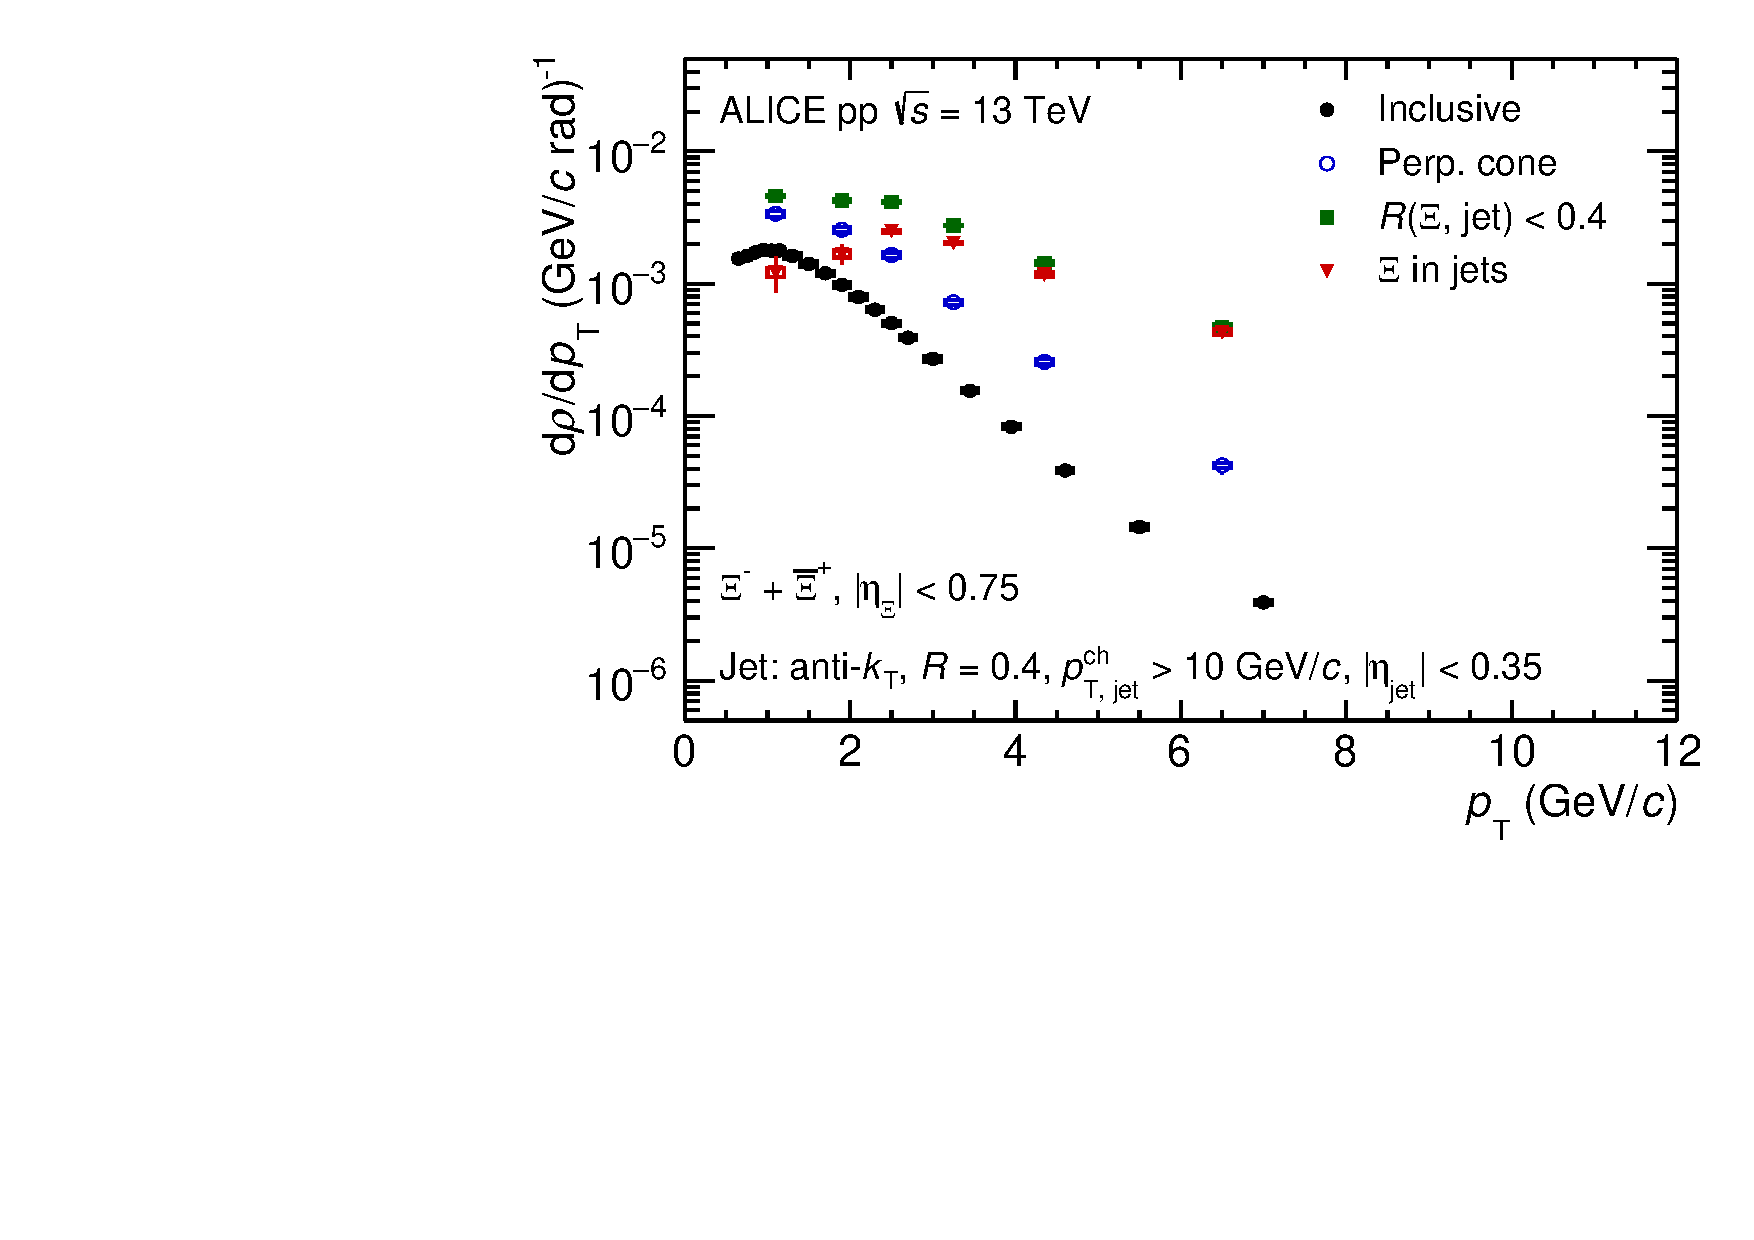
\includegraphics[width=.4\textwidth]{cf04_3}
		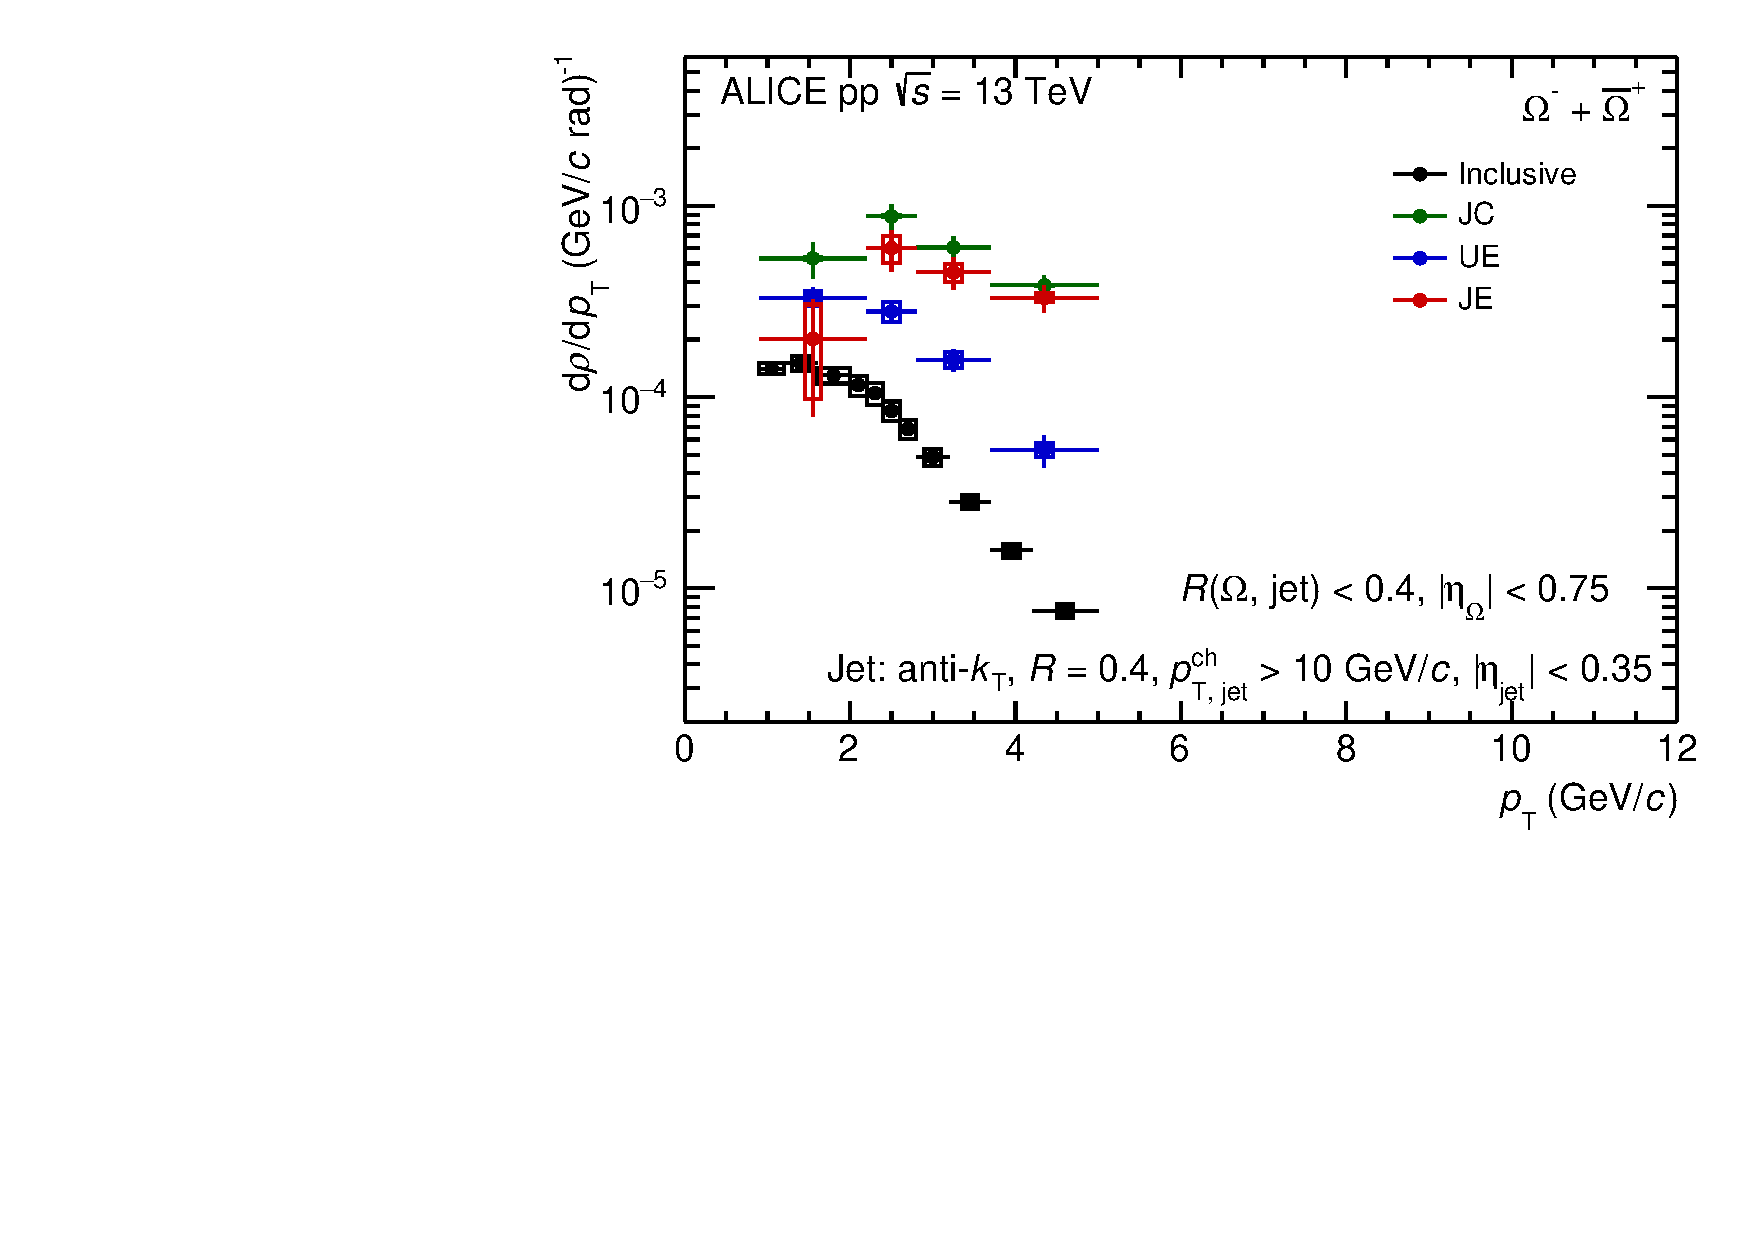
\includegraphics[width=.4\textwidth]{cf04_4}
	\end{center}
	\caption{$\pT$-differential density of $\kzero$, $\lmb + \almb$, $\X + \Ix$ and $\Om + \Mo$ in \pp at \thirteen. In those plots, the black point represent particles witch from minimum bias events, the green point represent particles which from the jet cones, the blue point represent particles within perpendicular cone of jet which associated with the underlying event and the red point represent the particle from the jet fragmentation.}
	\label{fig:ppSpect}
\end{figure}
\begin{figure}[!ht]
	\begin{center}
		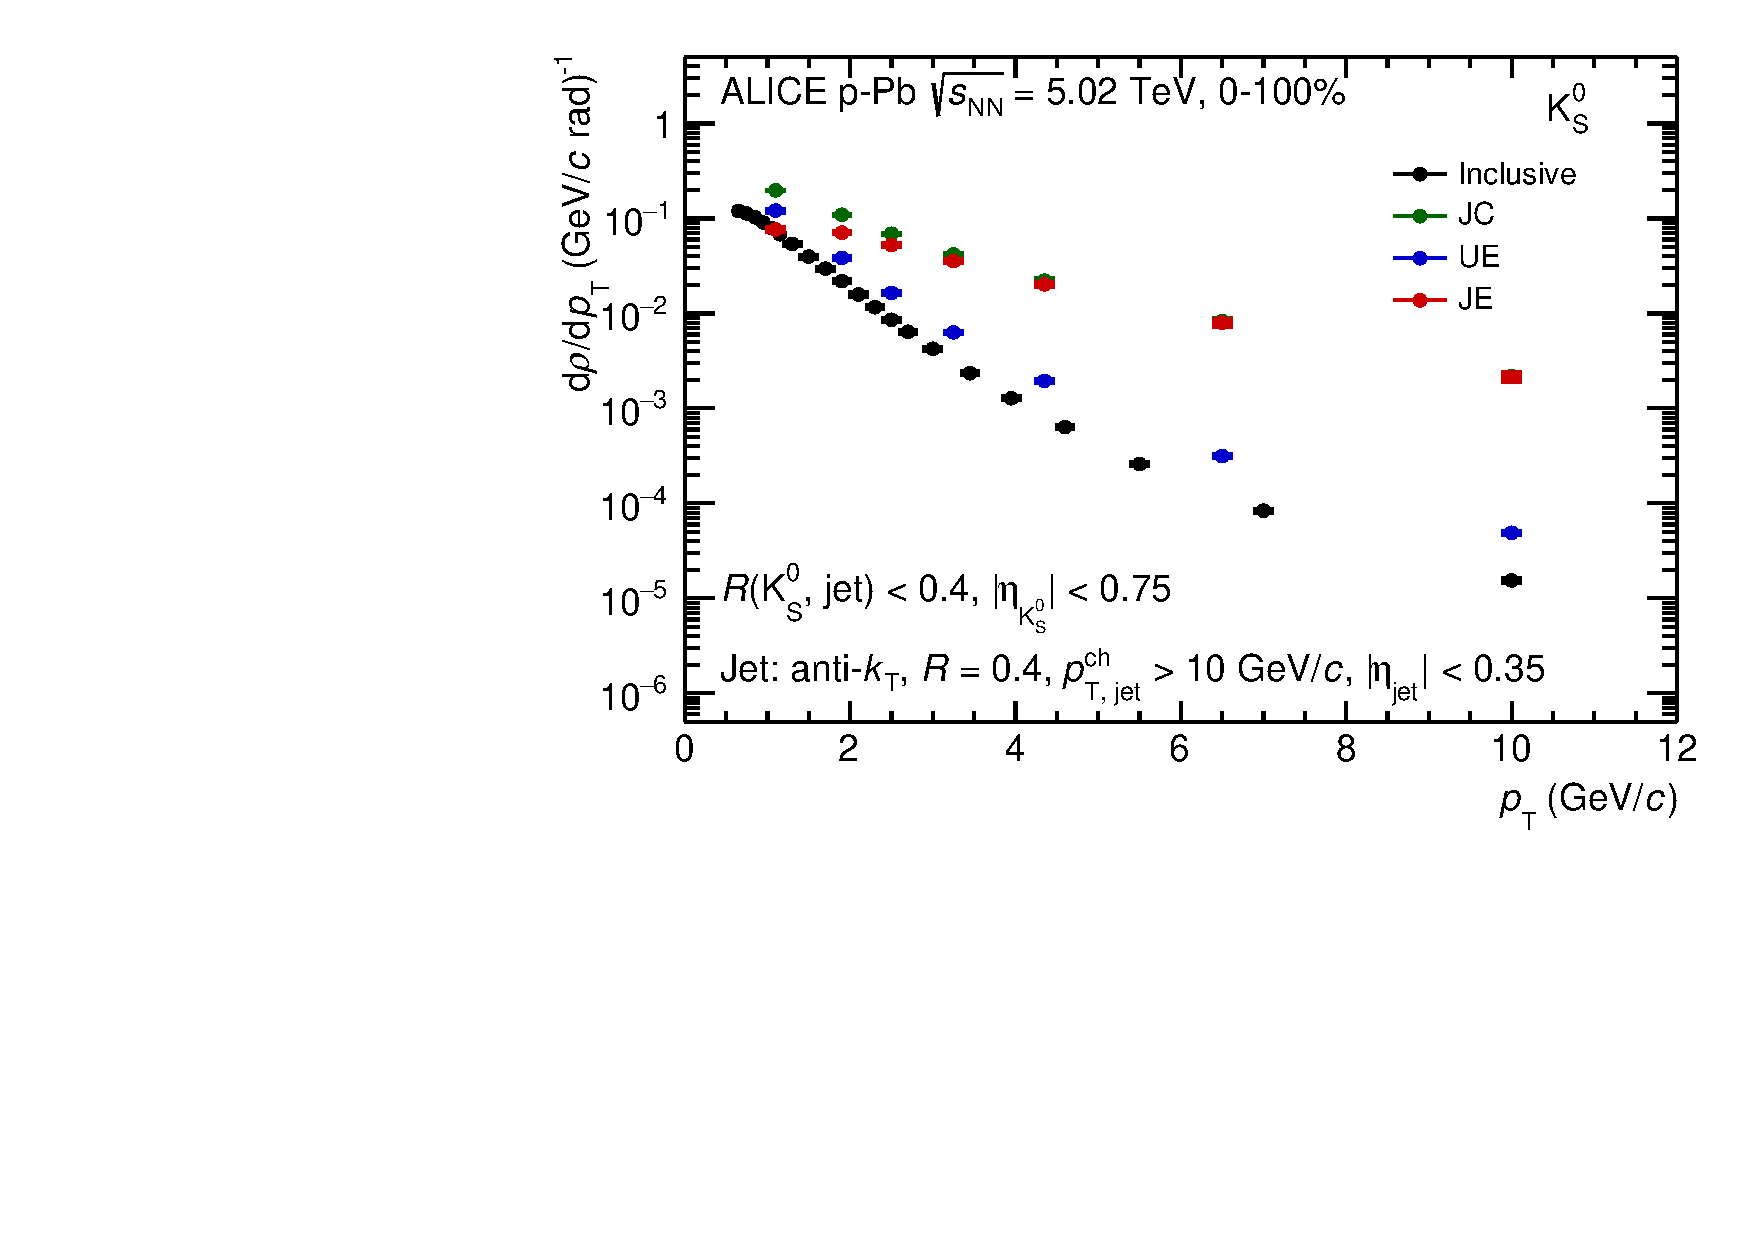
\includegraphics[width=.4\textwidth]{cf05_1}
		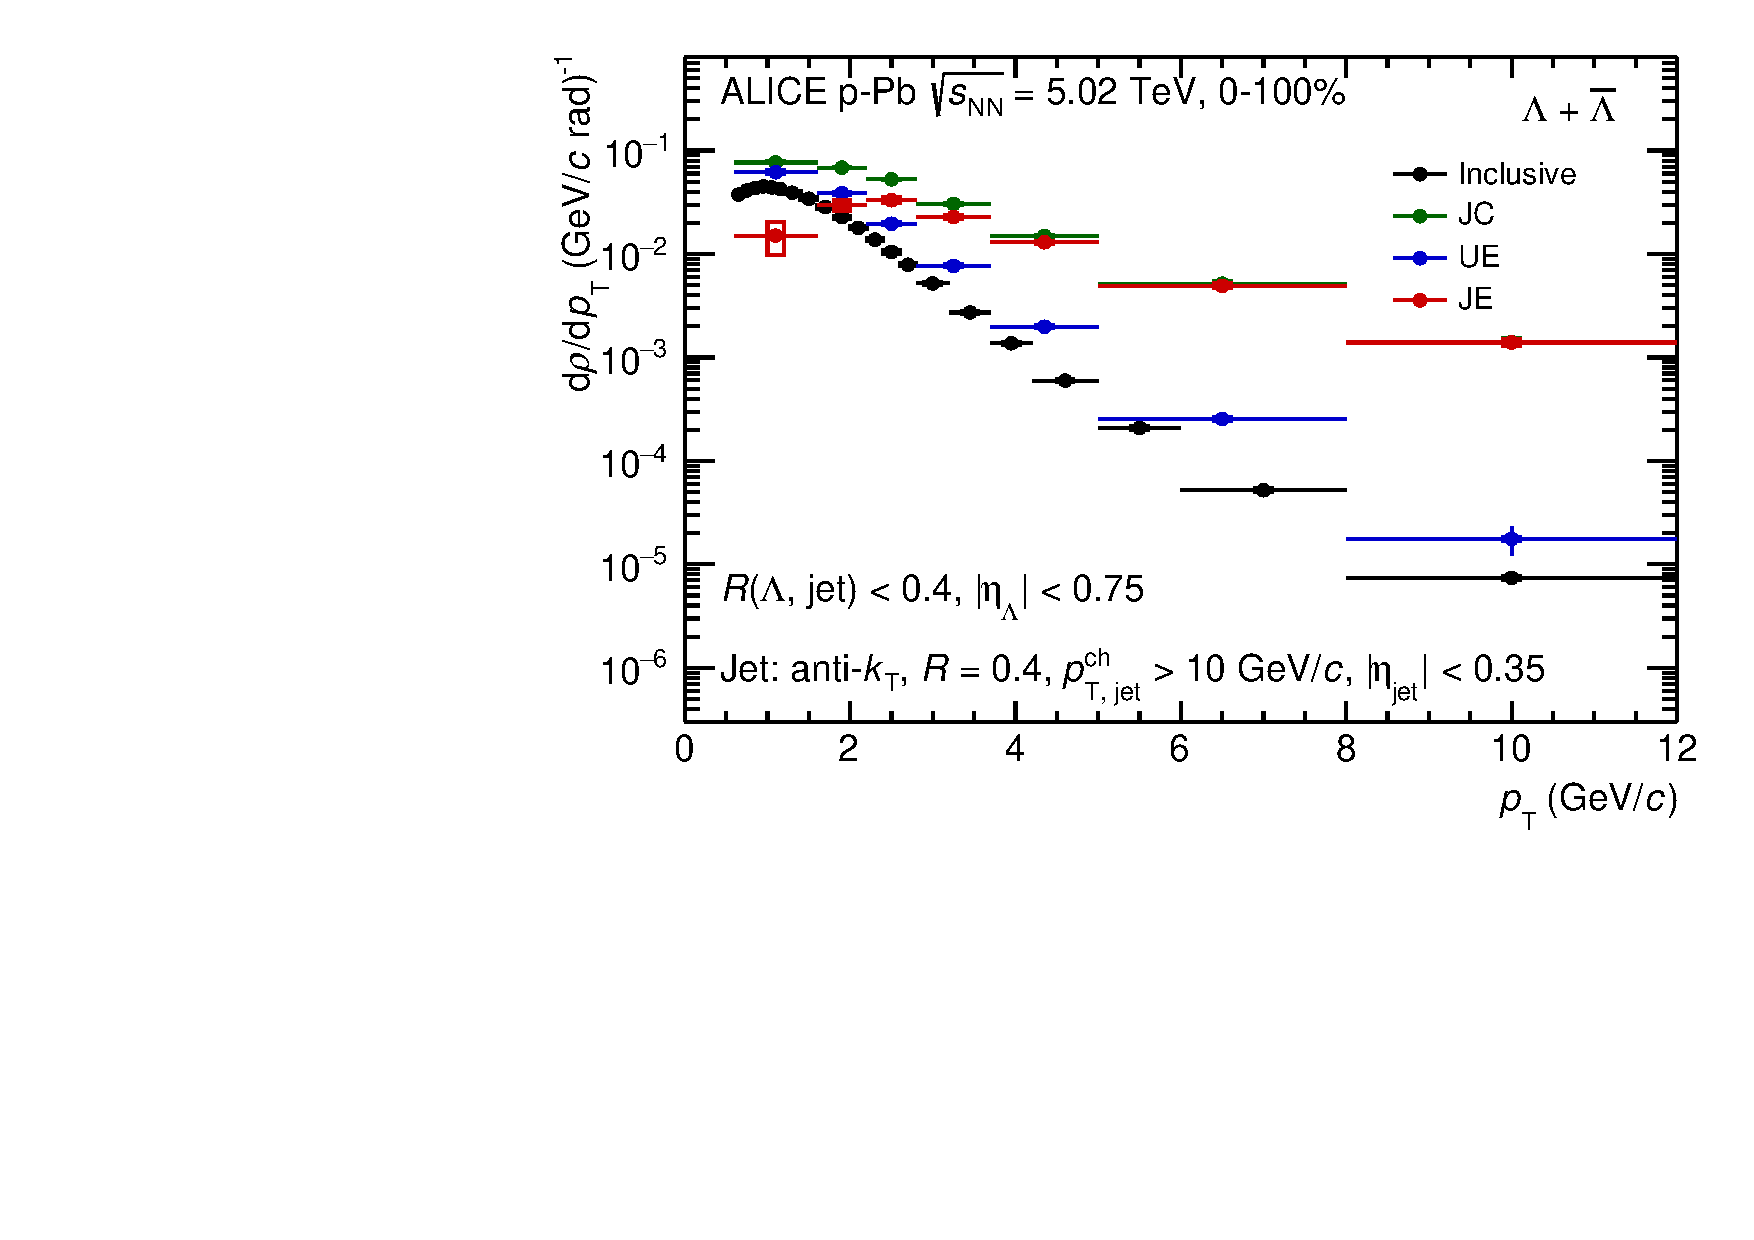
\includegraphics[width=.4\textwidth]{cf05_2}
		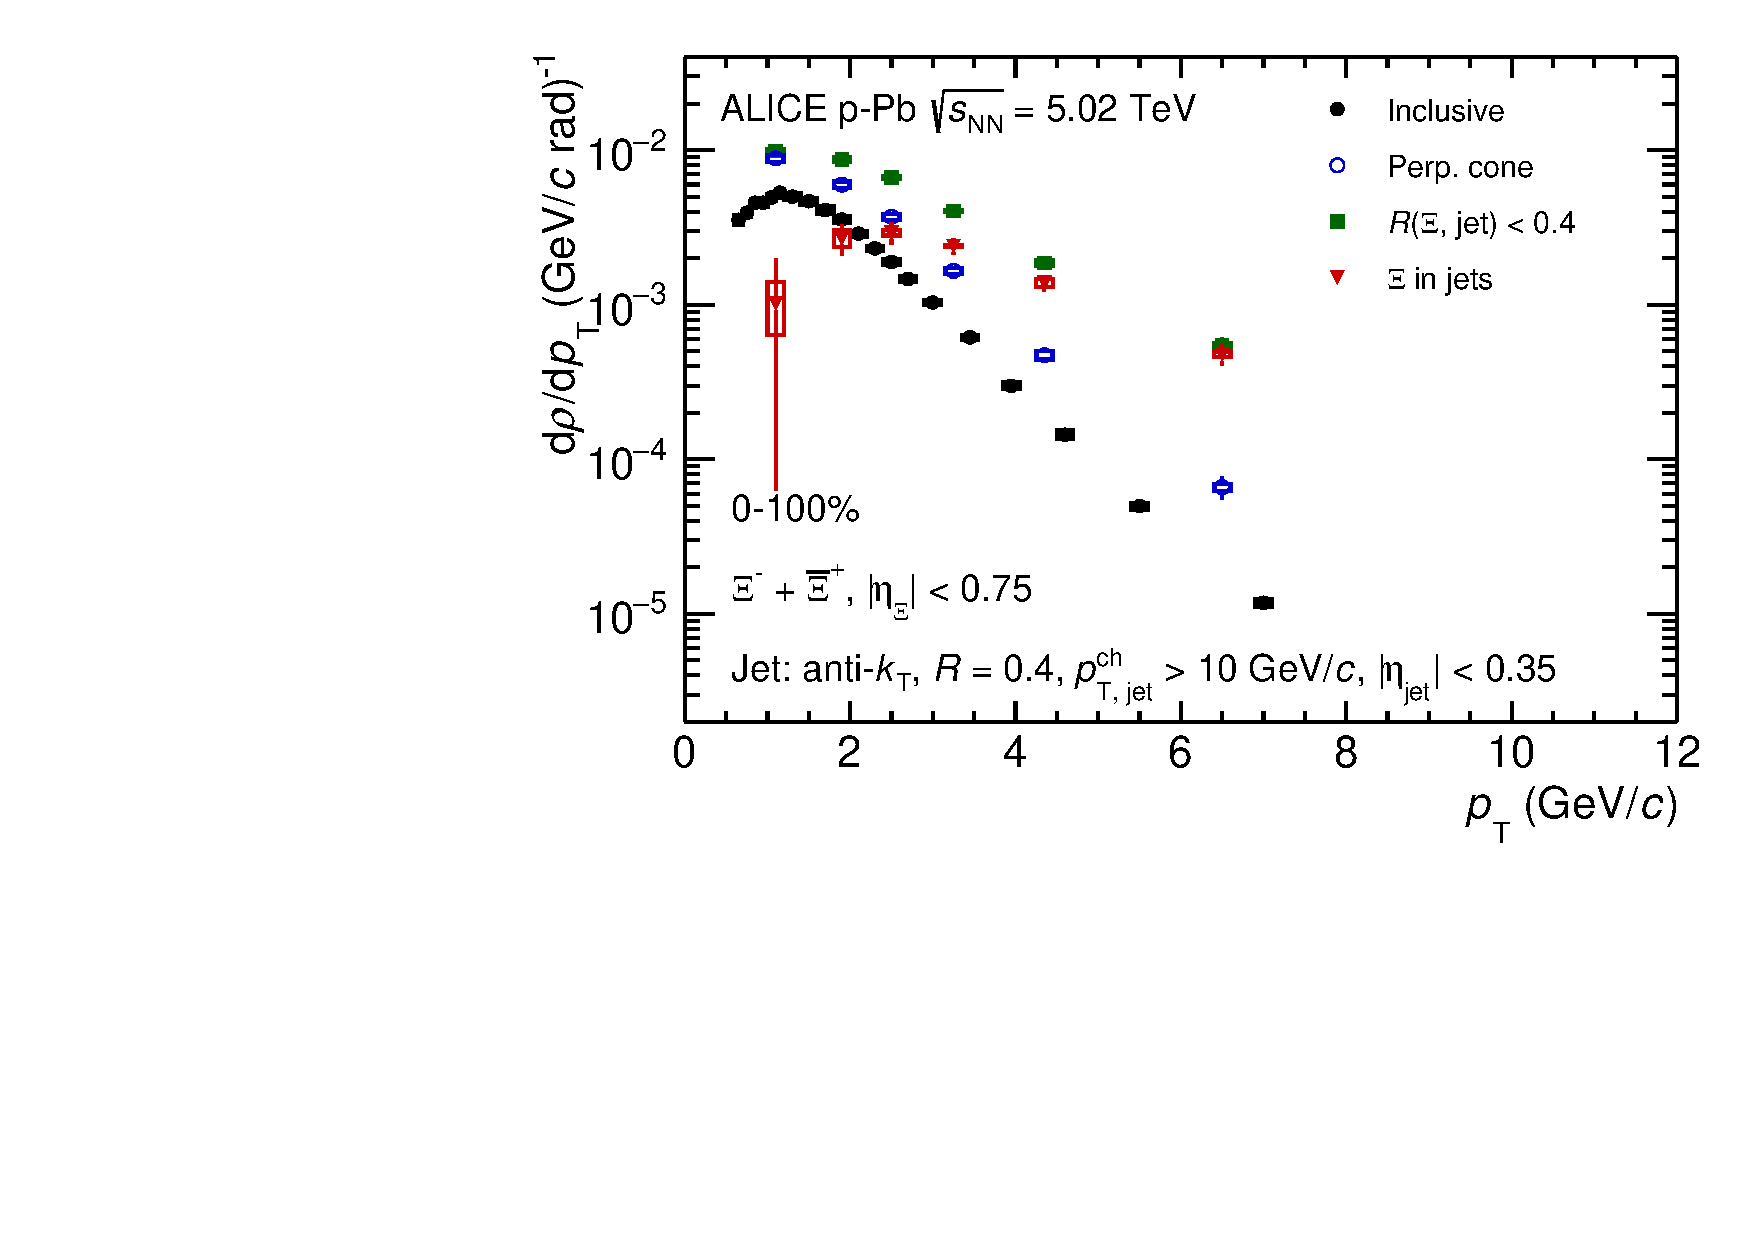
\includegraphics[width=.4\textwidth]{cf05_3}
		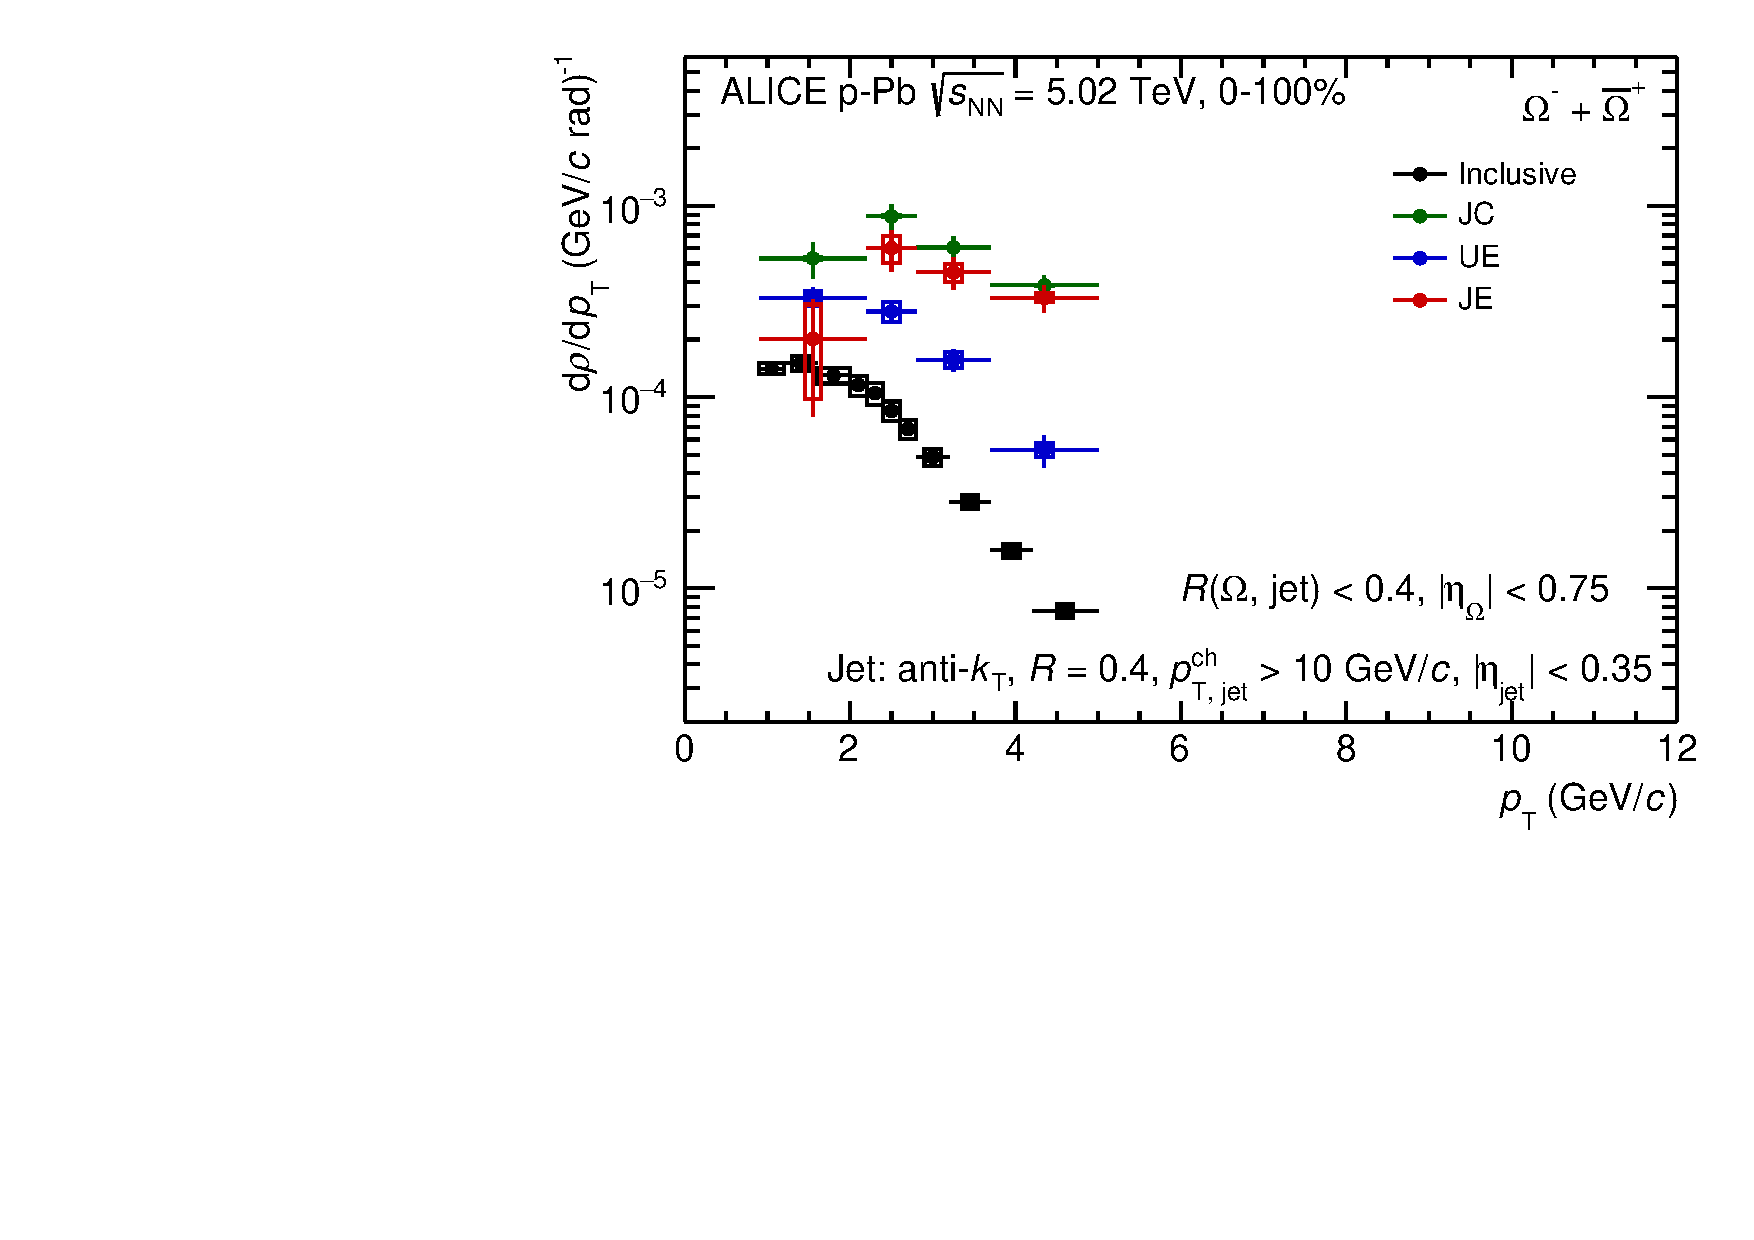
\includegraphics[width=.4\textwidth]{cf05_4}
	\end{center}
	\caption{$\pT$-differential density of $\kzero$, $\lmb + \almb$, $\X + \Ix$ and $\Om + \Mo$ in 0-100\% in \pPb at \fivenn. In those plots, the black point depicts particles witch from minimum bias events, the green point depicts particles which from the jet cones, the blue point depicts particles within perpendicular cone of jet which associated with the underlying event and the red point depicts the particle from the jet fragmentation.}
	\label{fig:pPbSpect}
\end{figure}

The $\pT$ distributions of $\kzero$, $\lmb + \almb$ and $\X + \Ix$ for the event classes defined in Tab.~\ref{tab:multi} are show in Fig.~\ref{fig:pPbSpectwCent}. The inclusive distributions become harder with increasing charged-particle multiplicity. Particles in JE, which generated by jet fragmentation, are systematically independent with centrality classes.
\begin{figure}[!ht]
	\begin{center}
		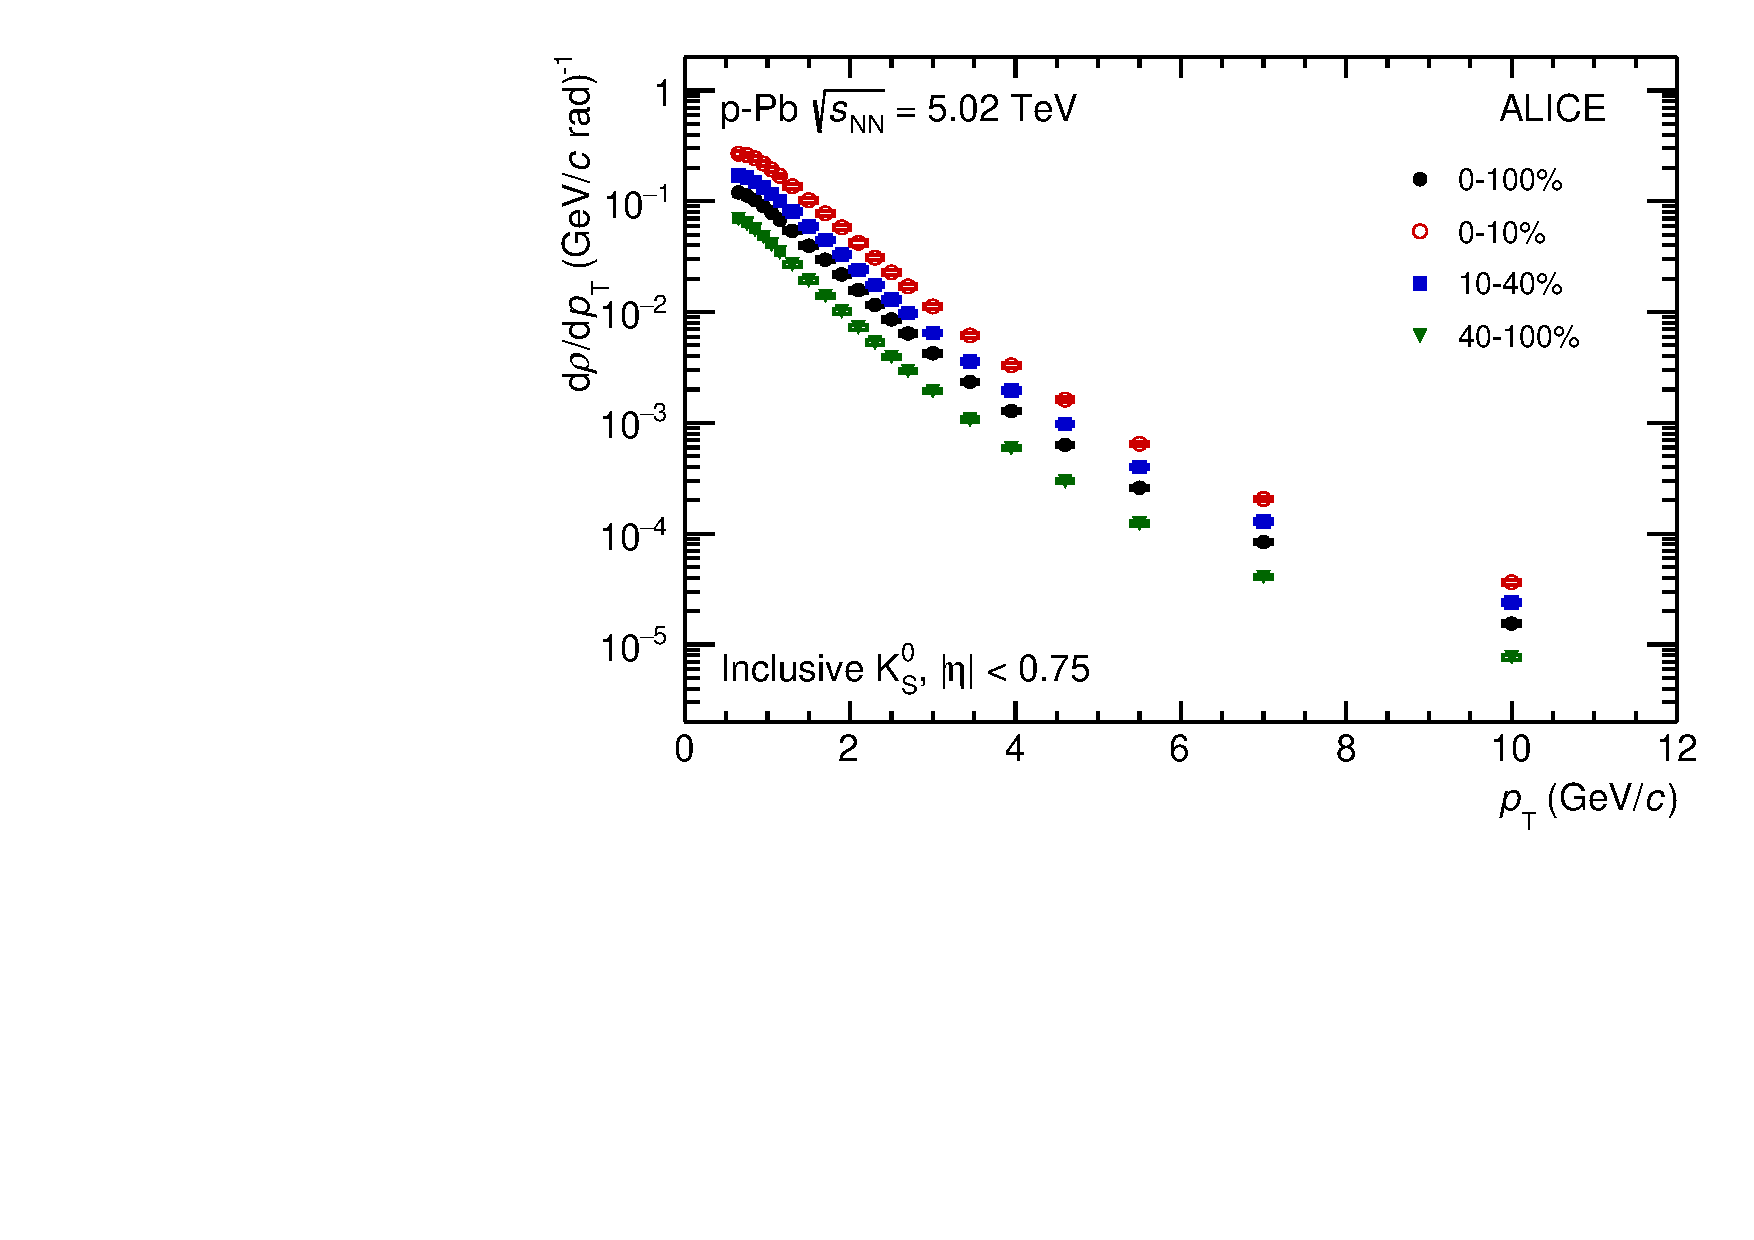
\includegraphics[width=.3\textwidth]{cf06_1}
		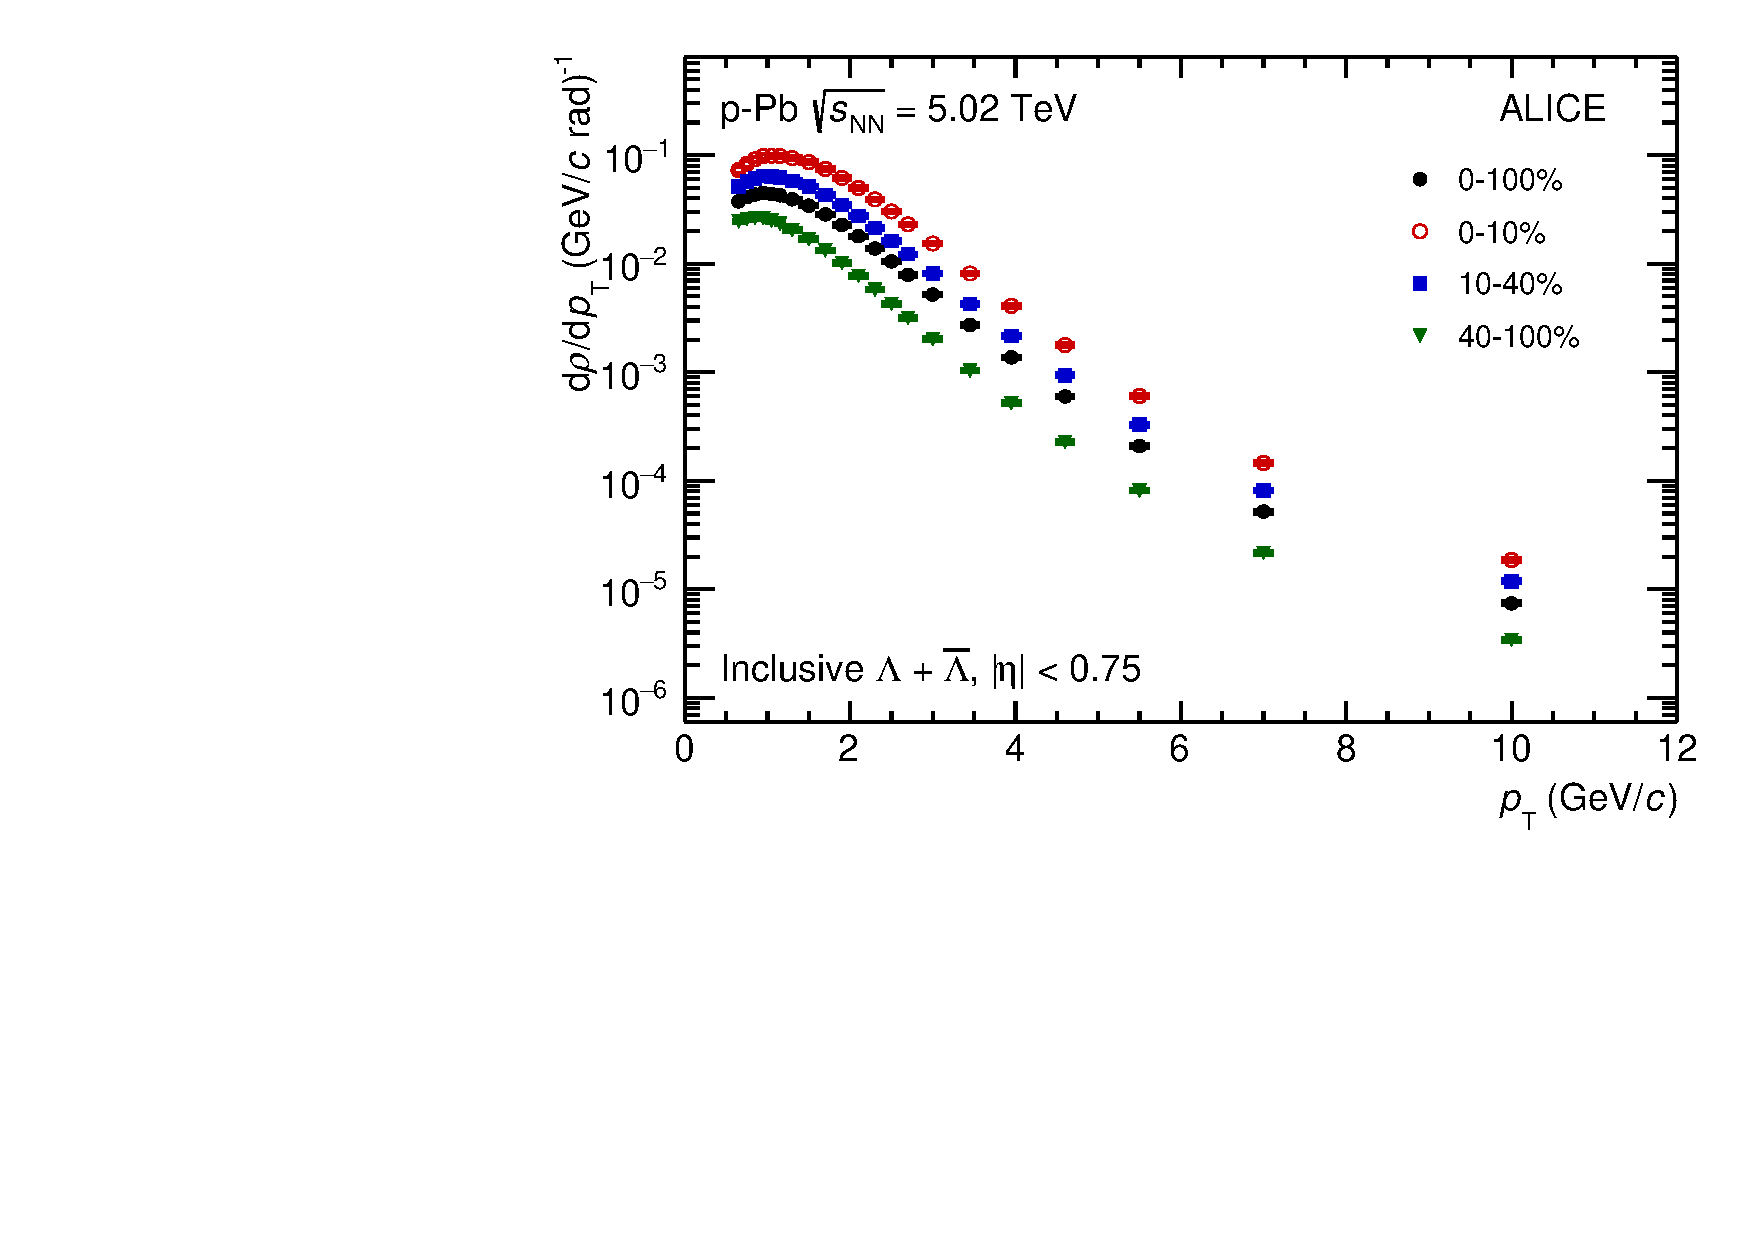
\includegraphics[width=.3\textwidth]{cf06_2}
		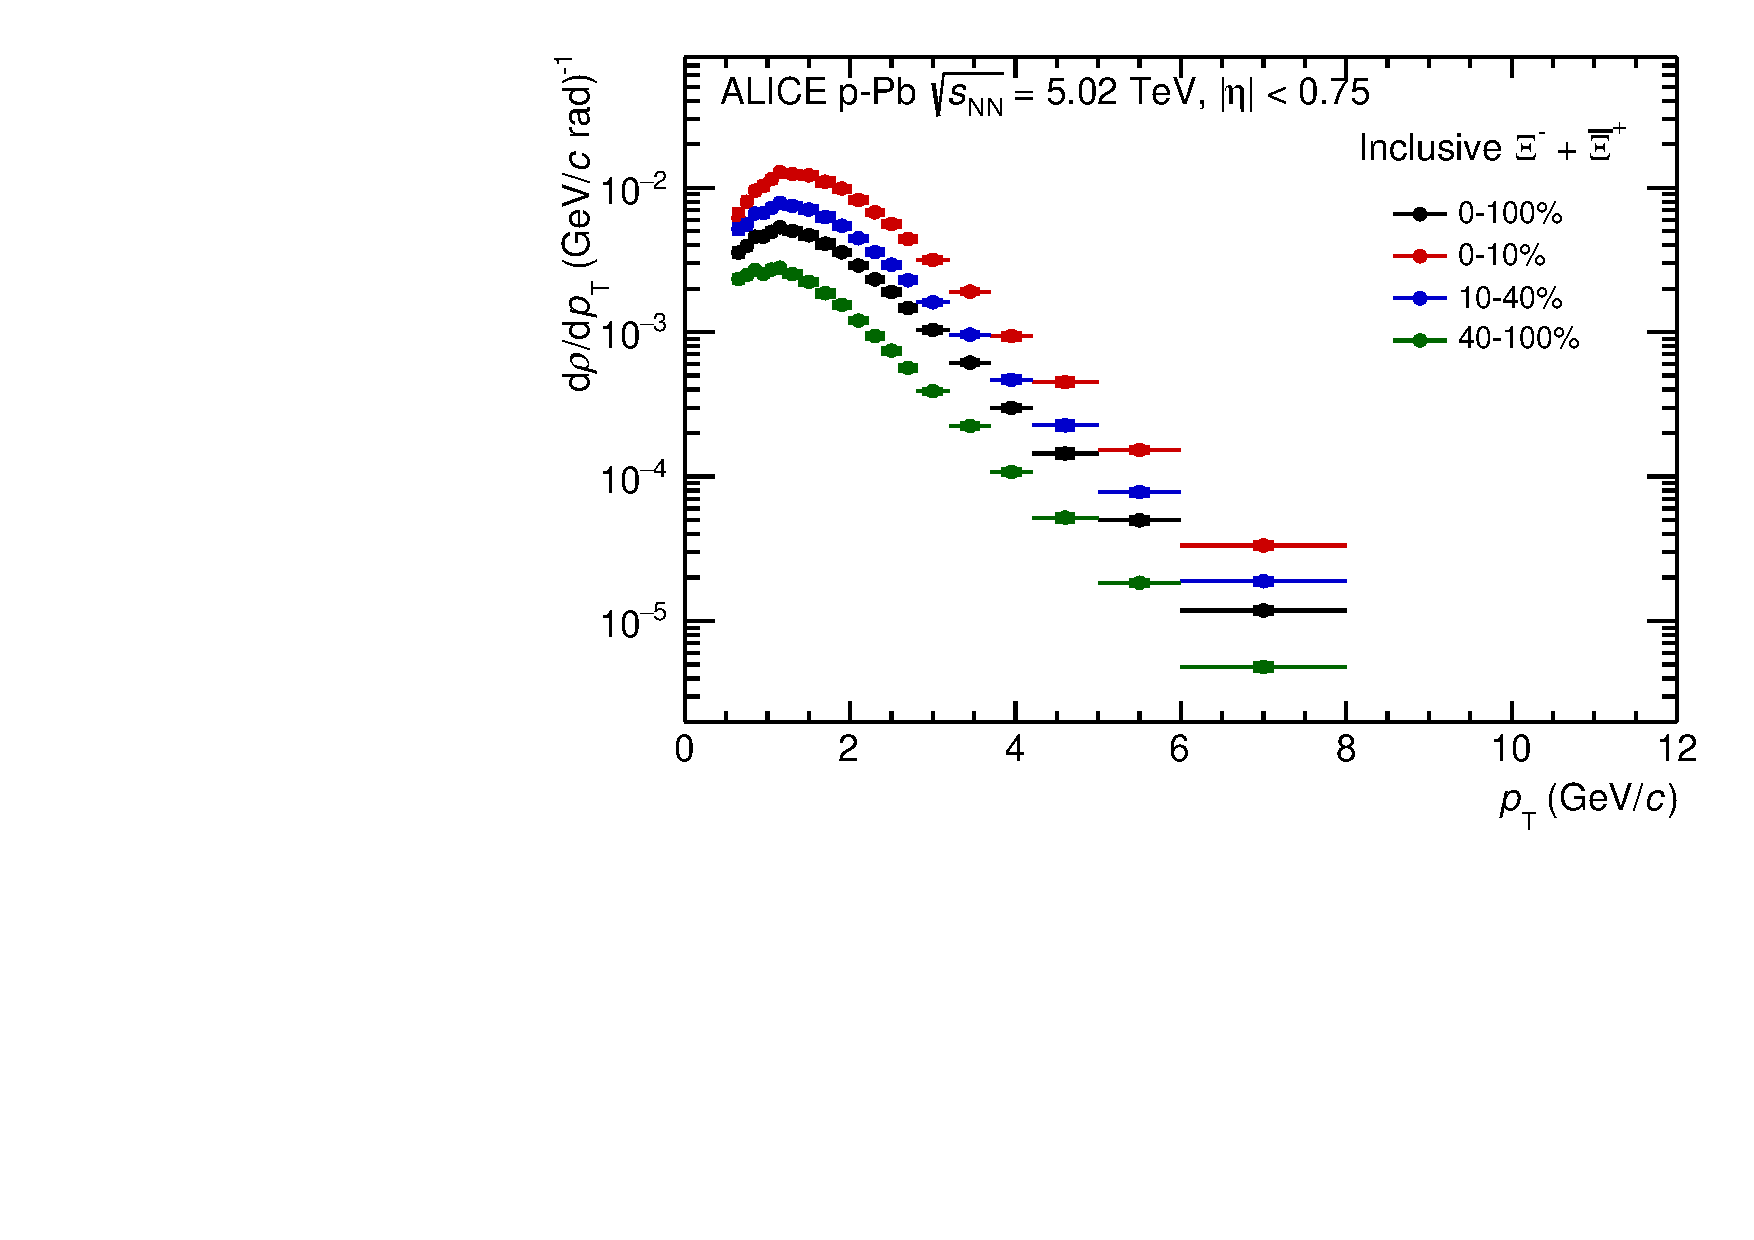
\includegraphics[width=.3\textwidth]{cf06_3}
		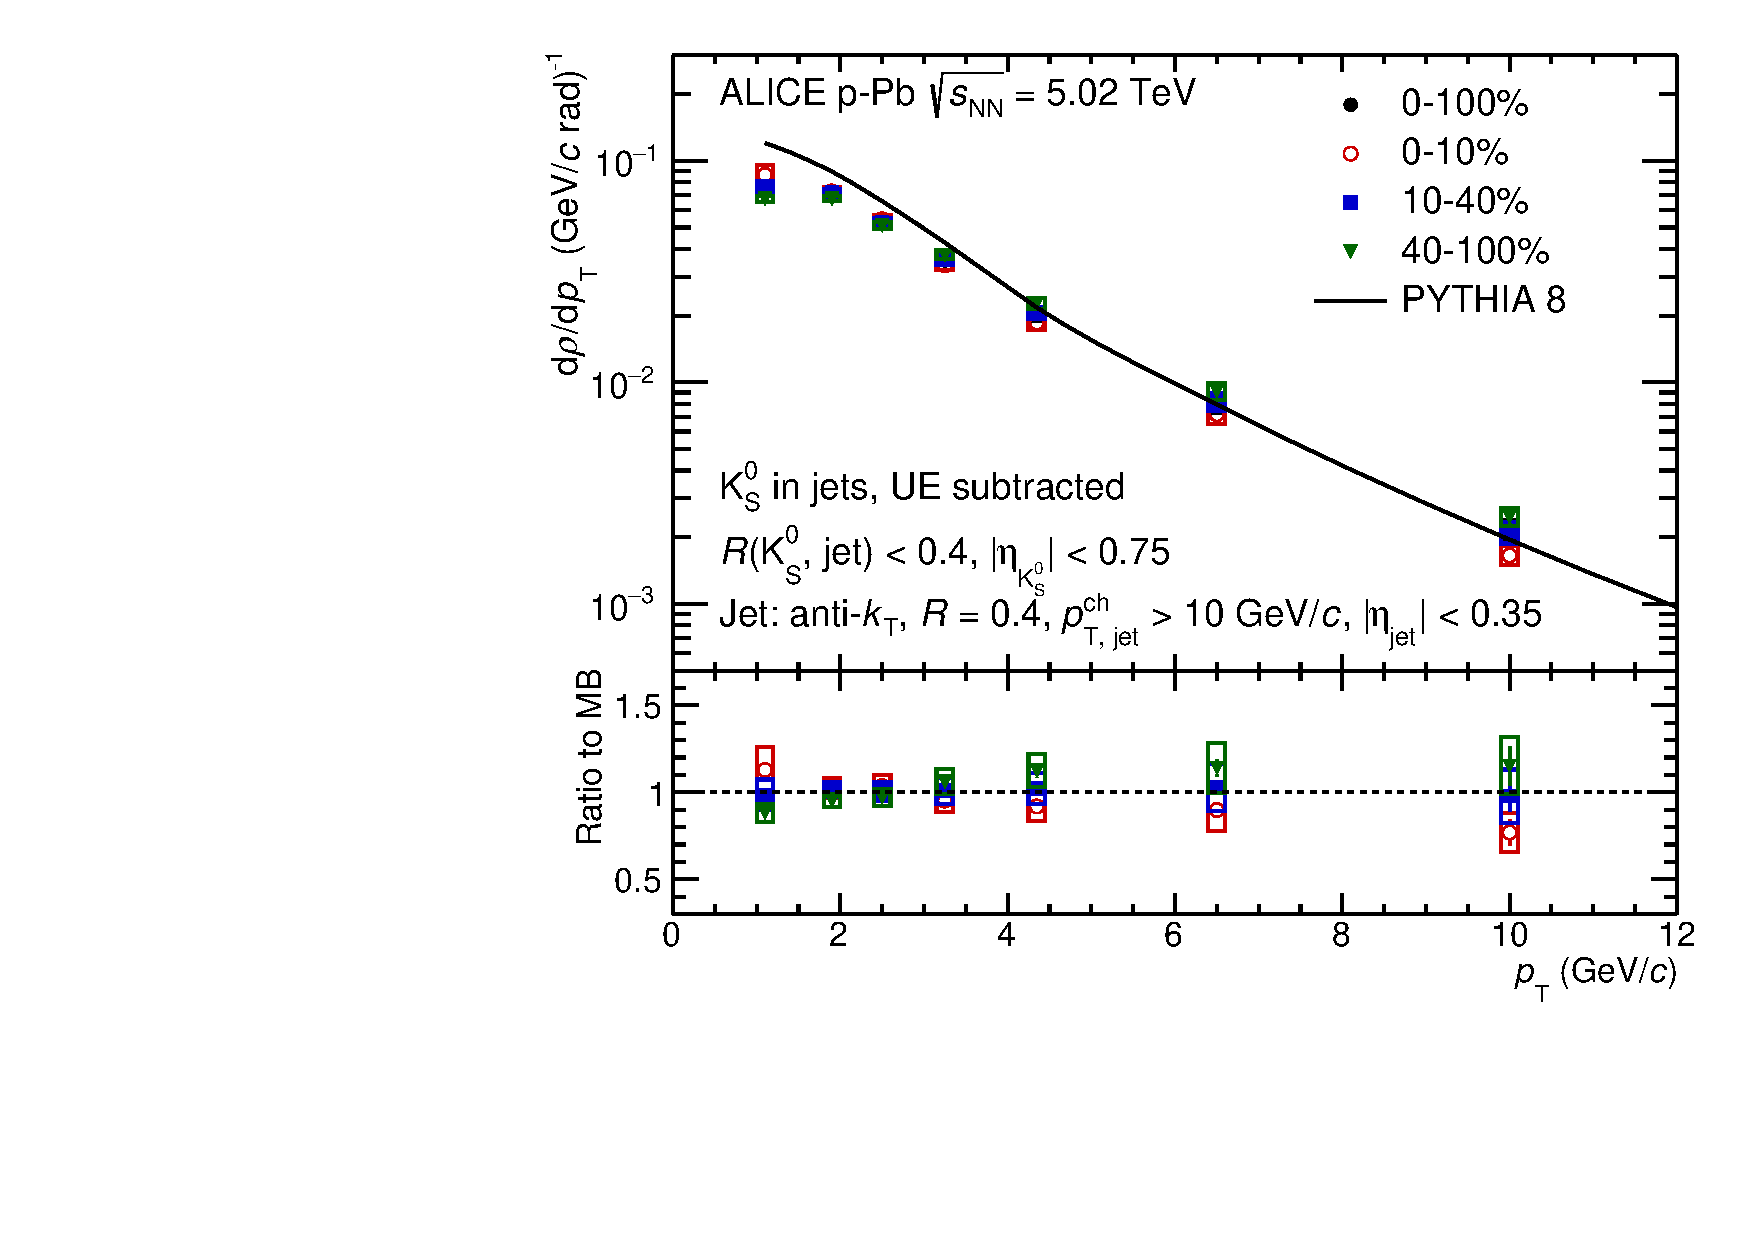
\includegraphics[width=.3\textwidth]{cf06_4}
		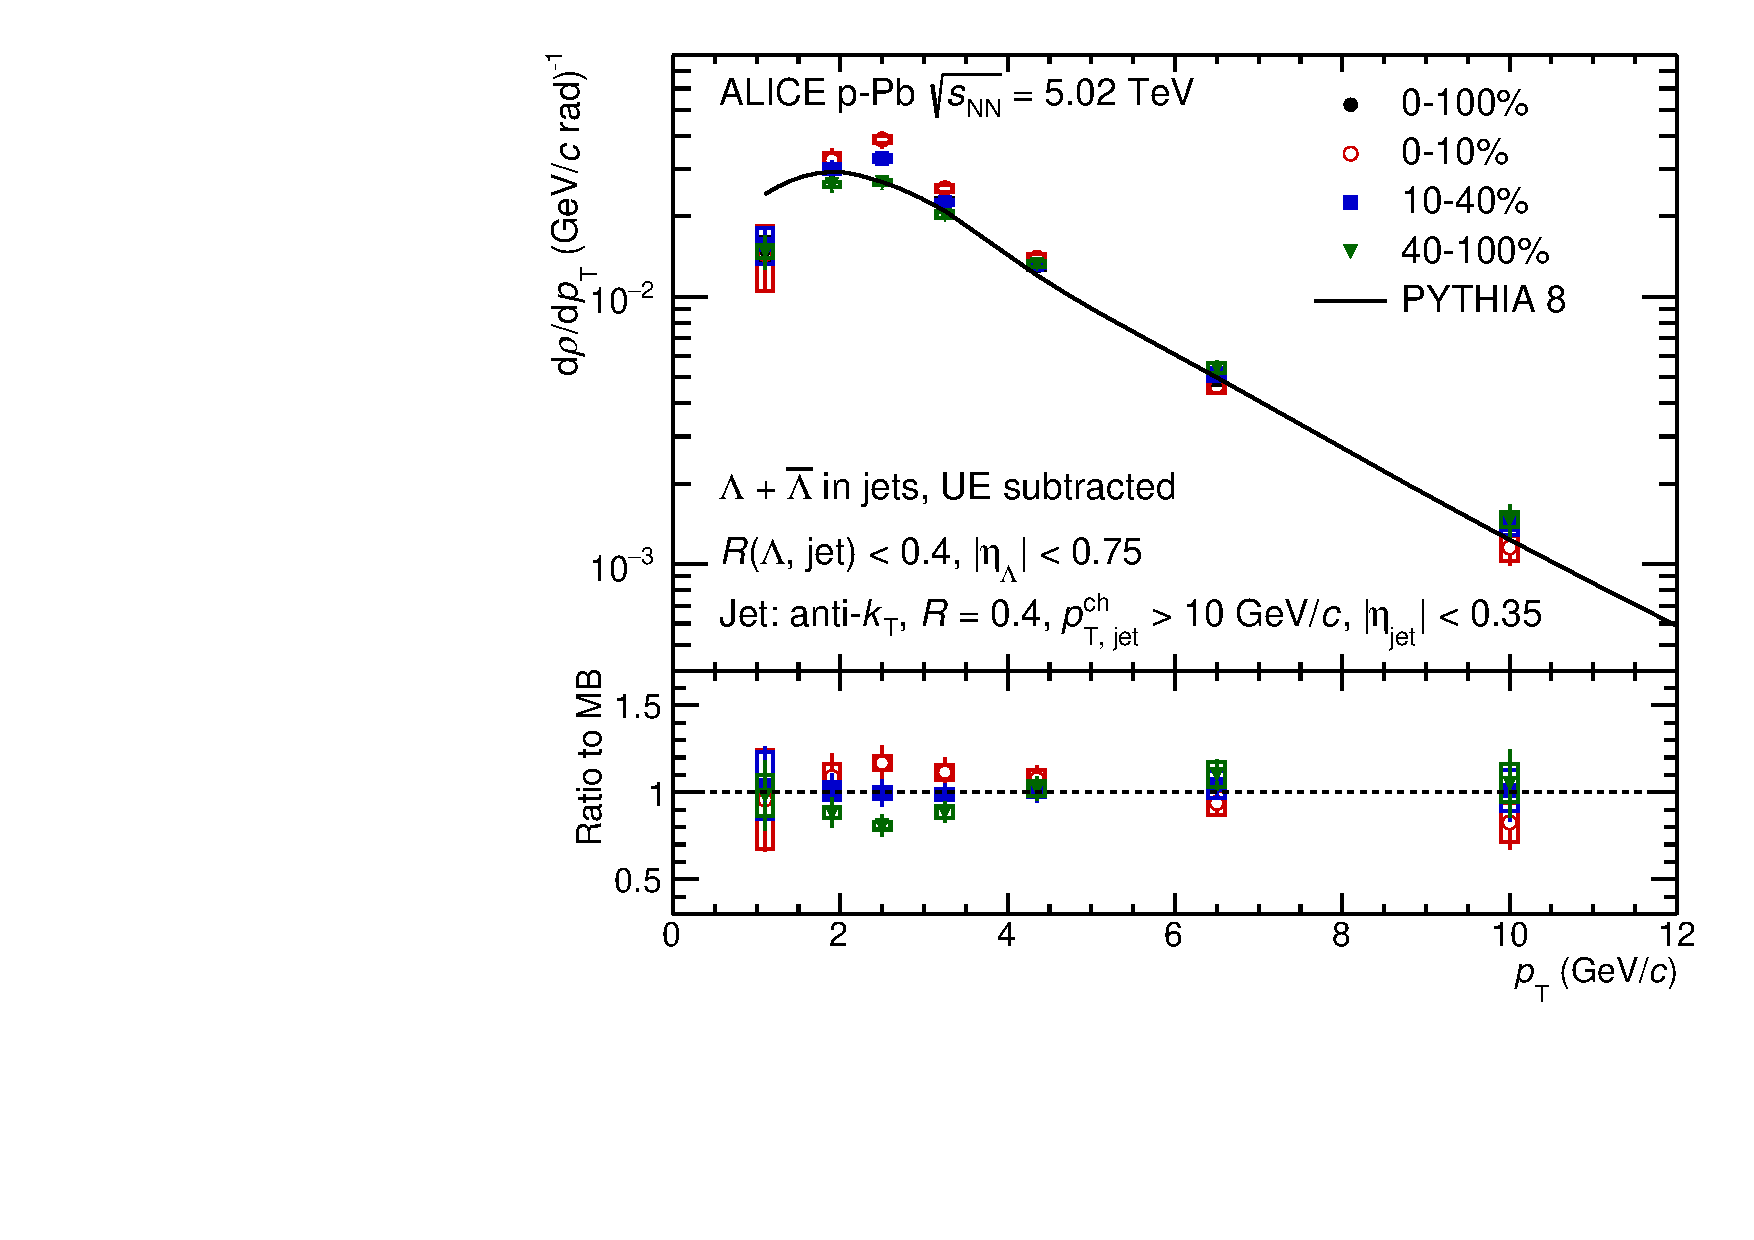
\includegraphics[width=.3\textwidth]{cf06_5}
		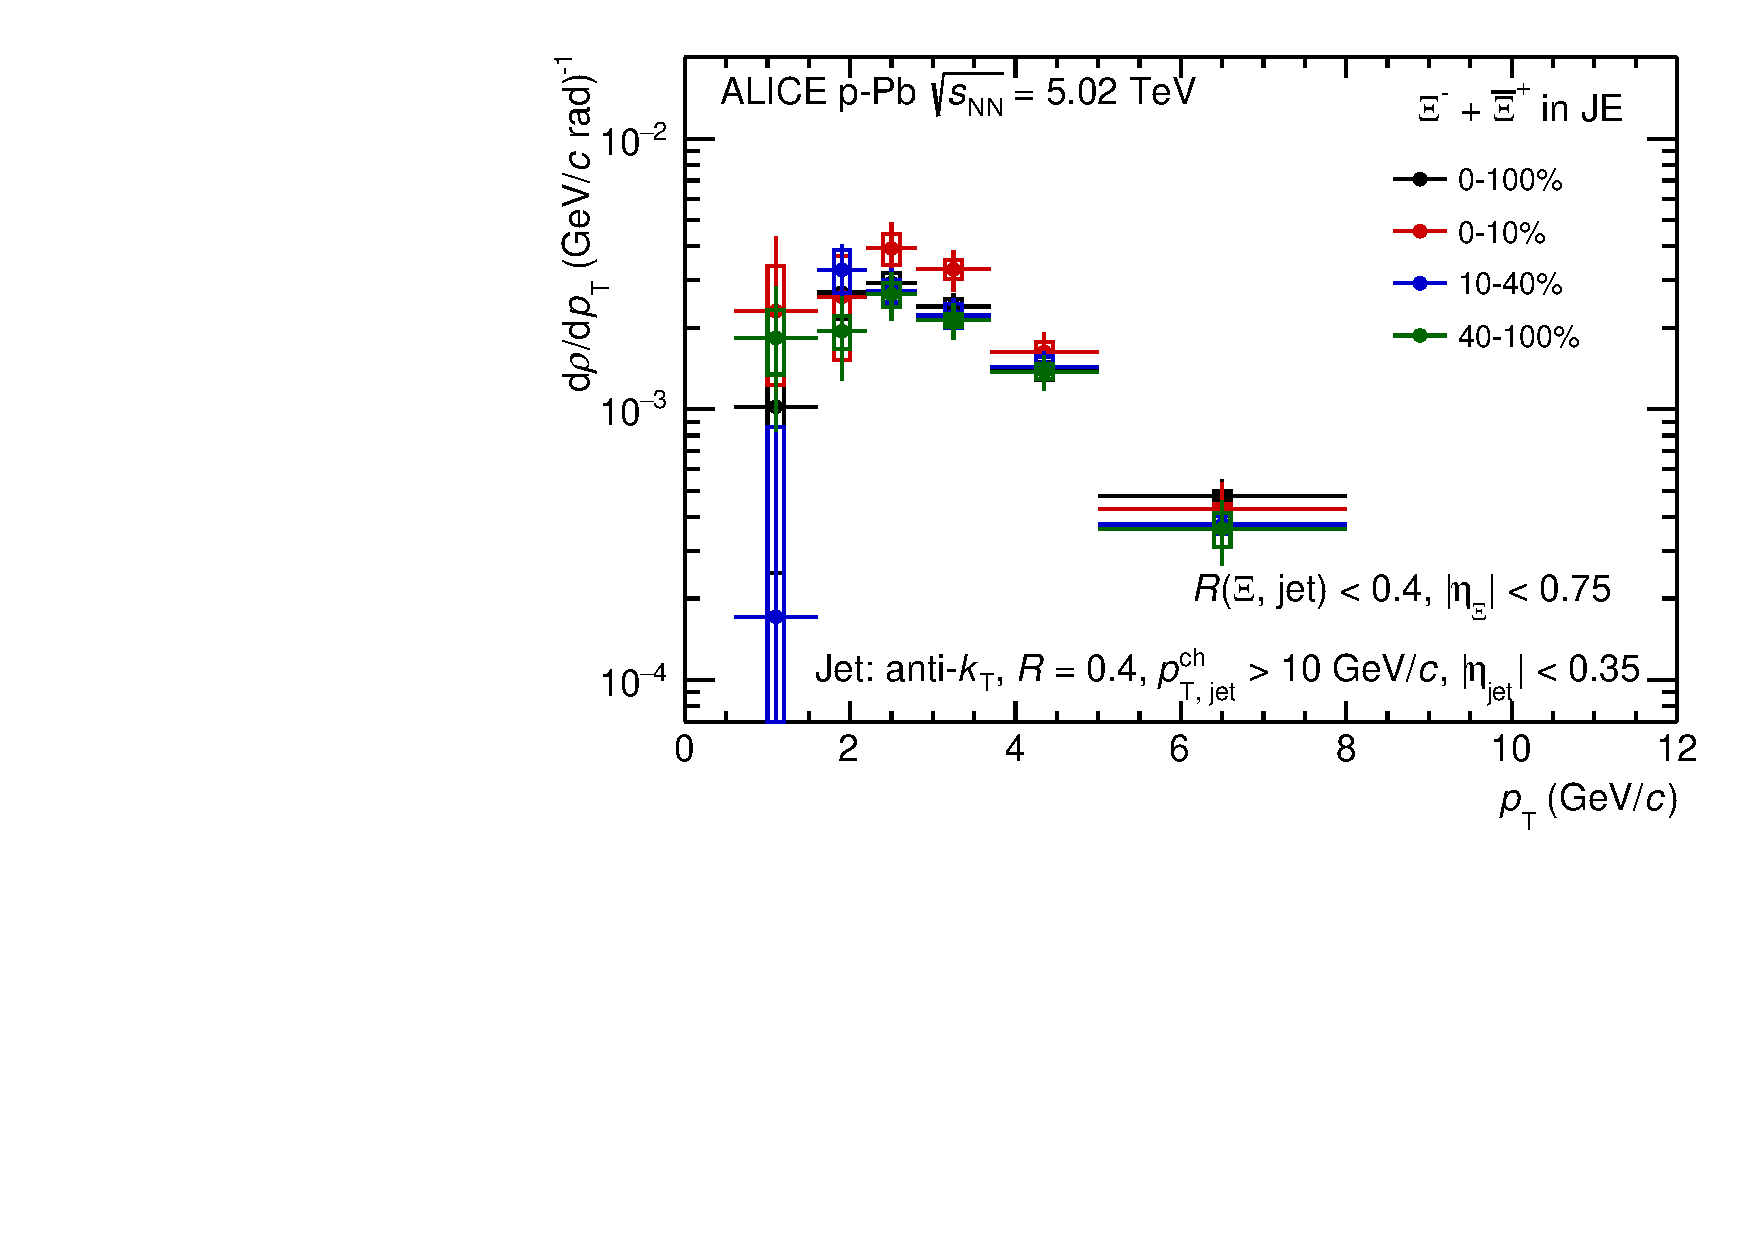
\includegraphics[width=.3\textwidth]{cf06_6}
	\end{center}
	\caption{$\pT$-differential density of $\kzero$, $\lmb + \almb$ and $\X + \Ix$ in different V0A event centrality classes in \pPb at \fivenn. Top panels show the inclusive particle and bottom panels show particles generated by jet fragmentation. The different centrality classes are depicted with different color.}
	\label{fig:pPbSpectwCent}
\end{figure}

\subsection{Baryon-to-meson and baryon-to-baryon ratios}
\label{subsec:ParRatios}
The $\lmb/\kzero$, $\Xi/\kzero$ and $\Omega/\kzero$ baryon-to-meson ratios and $\Xi/\lmb$, $\Omega/\lmb$ and $\Omega/\Xi$ baryon-to-baryon ratios are investigated as a function of $\pT$ for several selections in \pp and \pPb collisions. As can be seen in Figs.~\ref{fig:ppRatio} (\pp at \thirteen) and \ref{fig:pPbRatio} (\pPb at \fivenn, 0-100\%), the inclusive particle ratios have an enhancement at $\pT \sim 3 - 4 $~\GeVc. Additionally, the same case of particle ratios in underlying events can be observed. However, the particle ratios in jet are significantly lower than the inclusive and UE cases at low and intermediate $\pT$. Also the ratios in jet are approximately independent of $\pT$ beyond 2~\GeVc. This suggests that the ratios of baryon-to-meson and baryon-to-baryon enhancement at intermediate $\pT$ is not driven by the jet fragmentation.

\begin{figure}[!ht]
	\begin{center}
		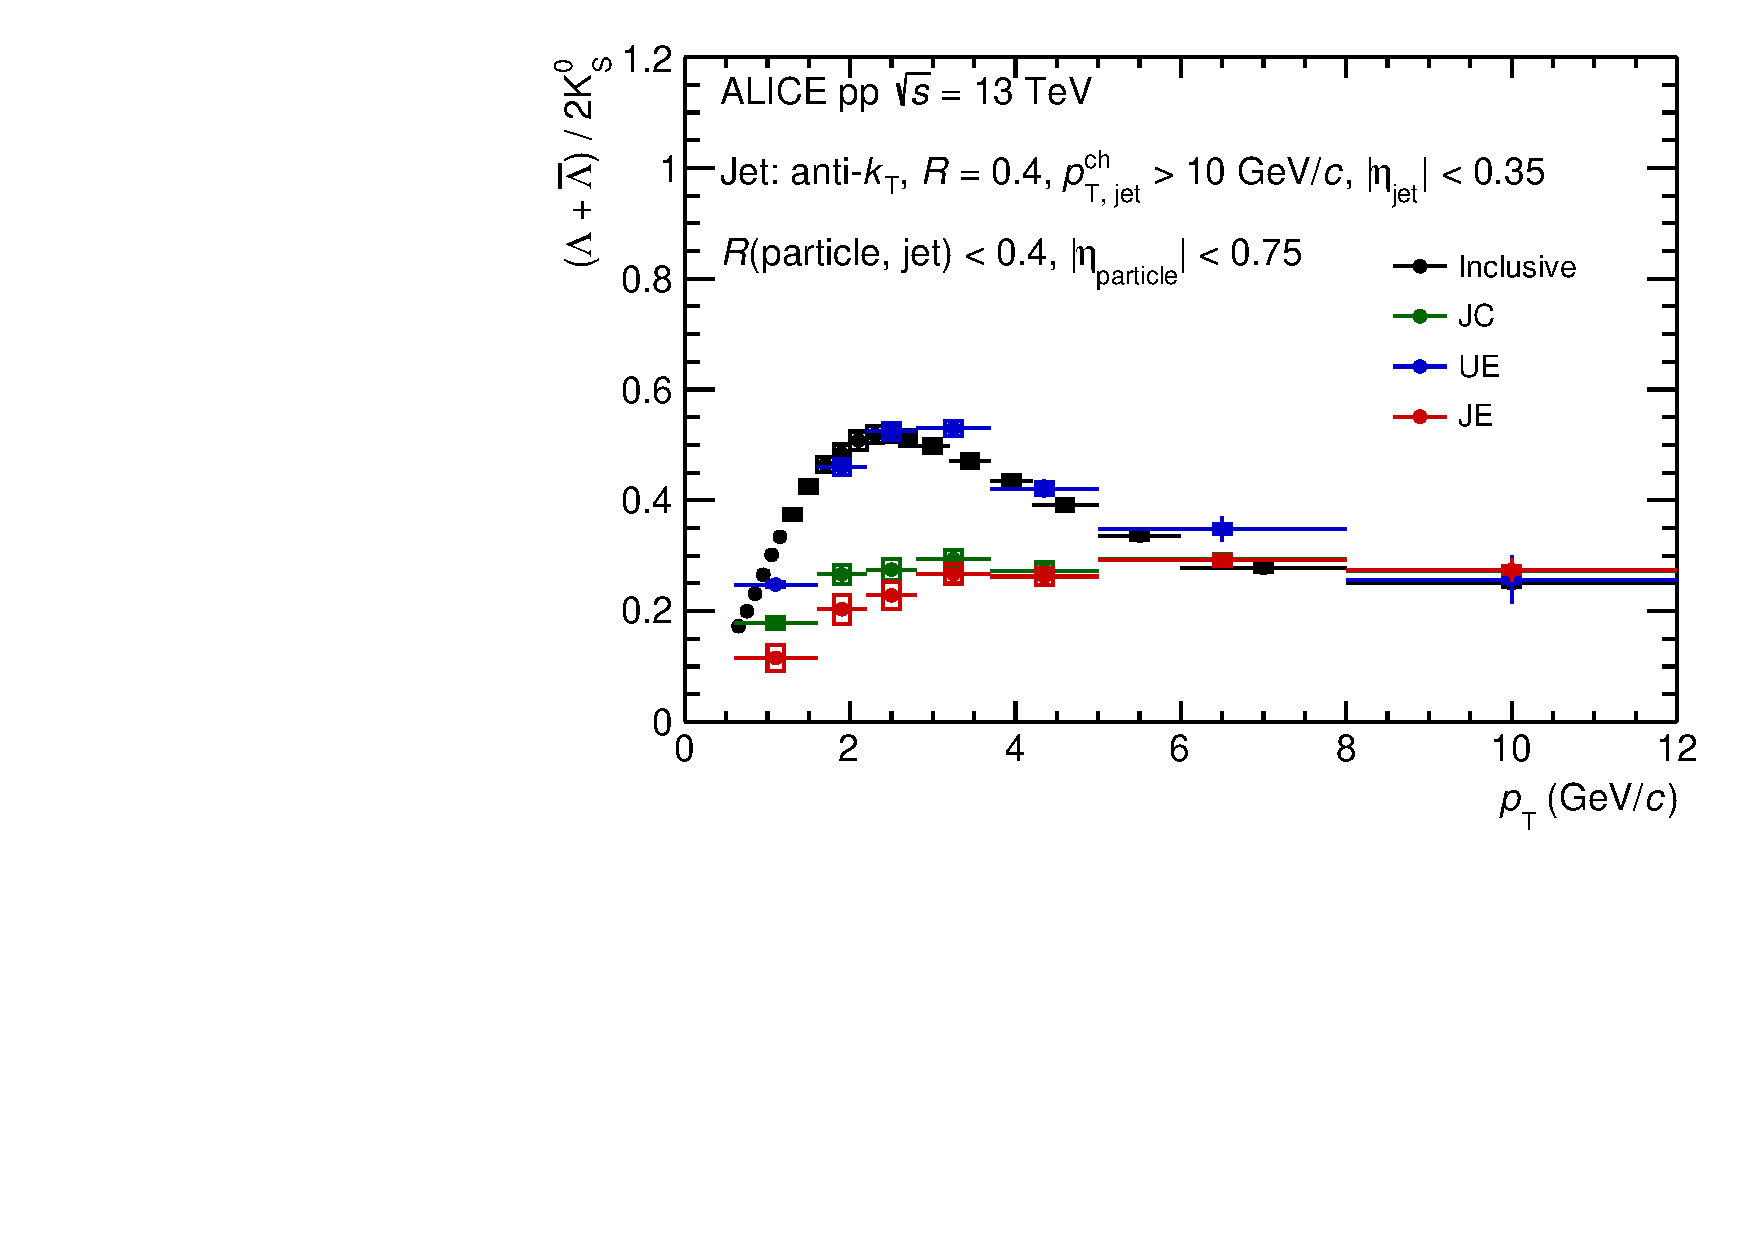
\includegraphics[width=.3\textwidth]{cf07_1}
		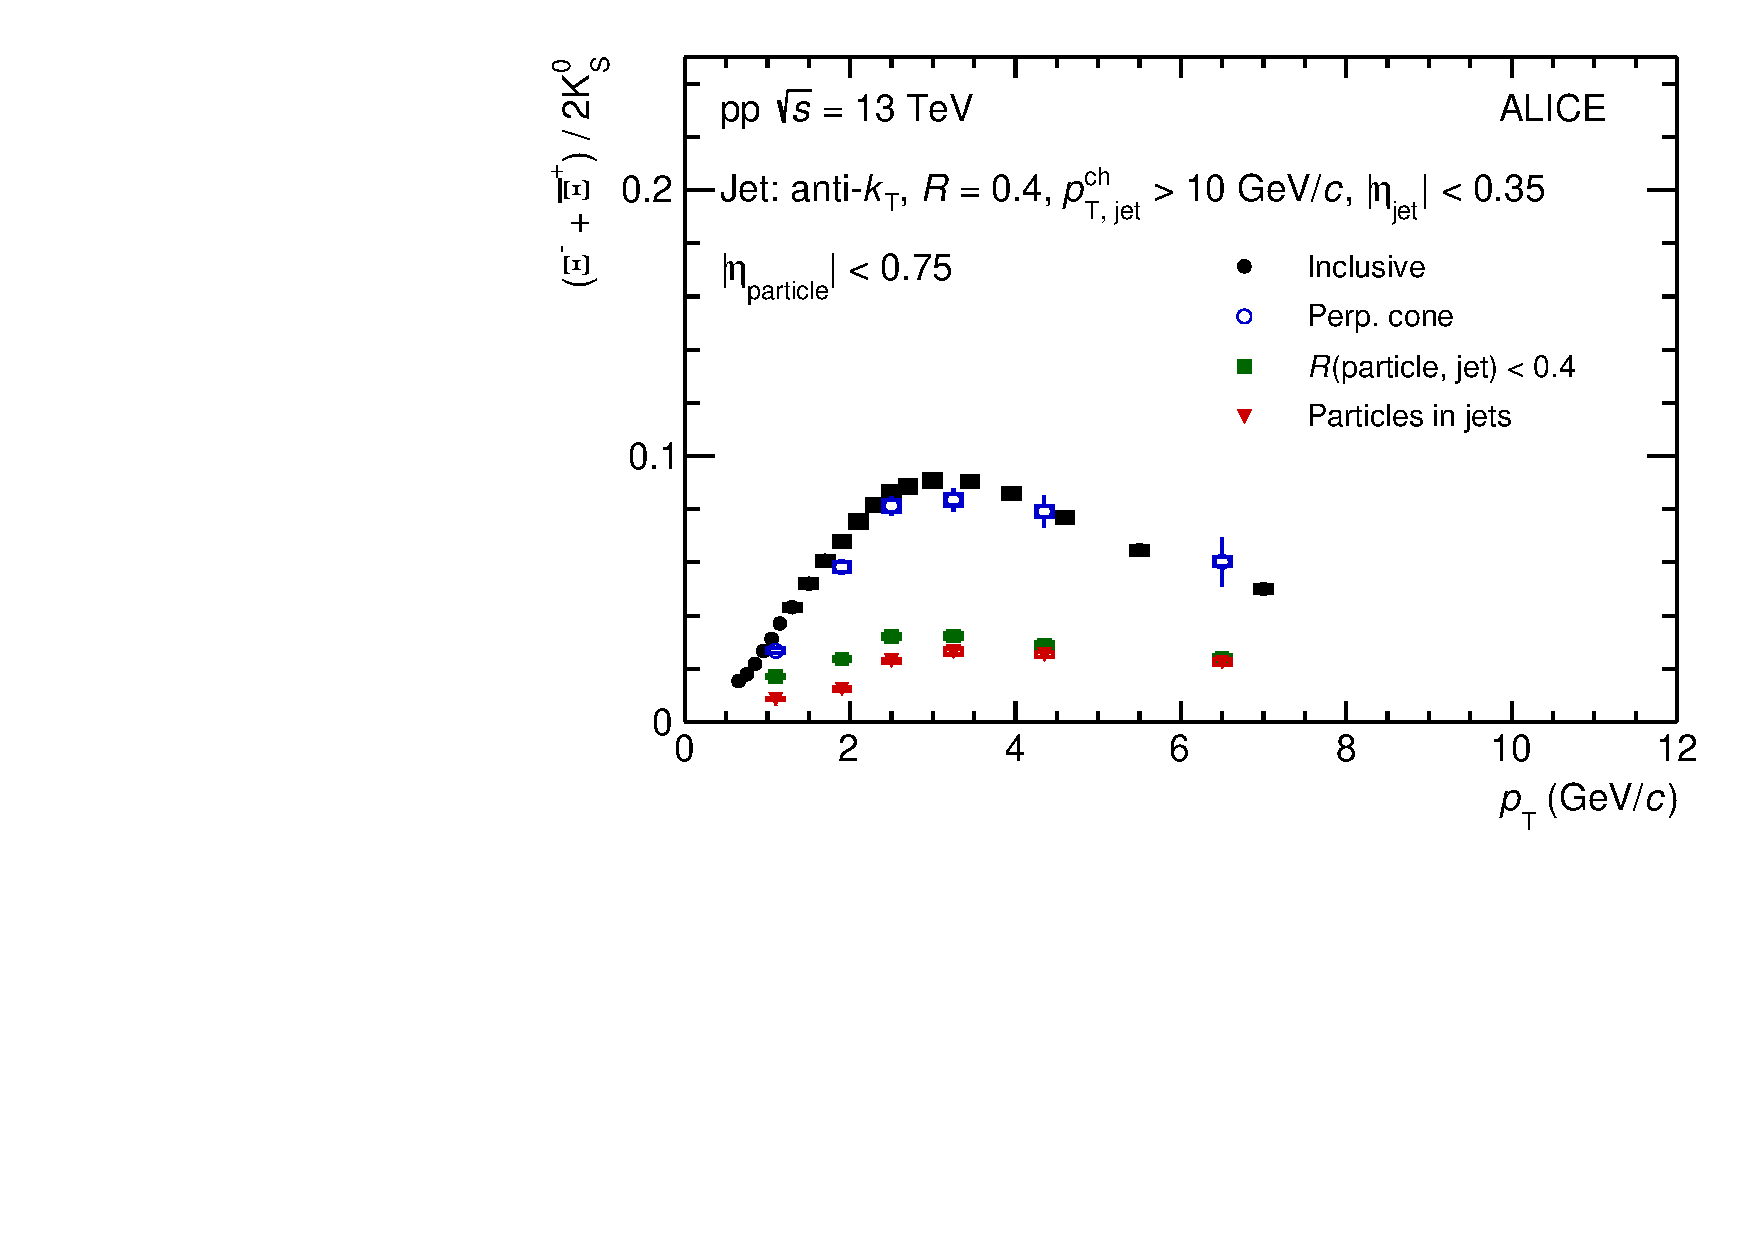
\includegraphics[width=.3\textwidth]{cf07_2}
		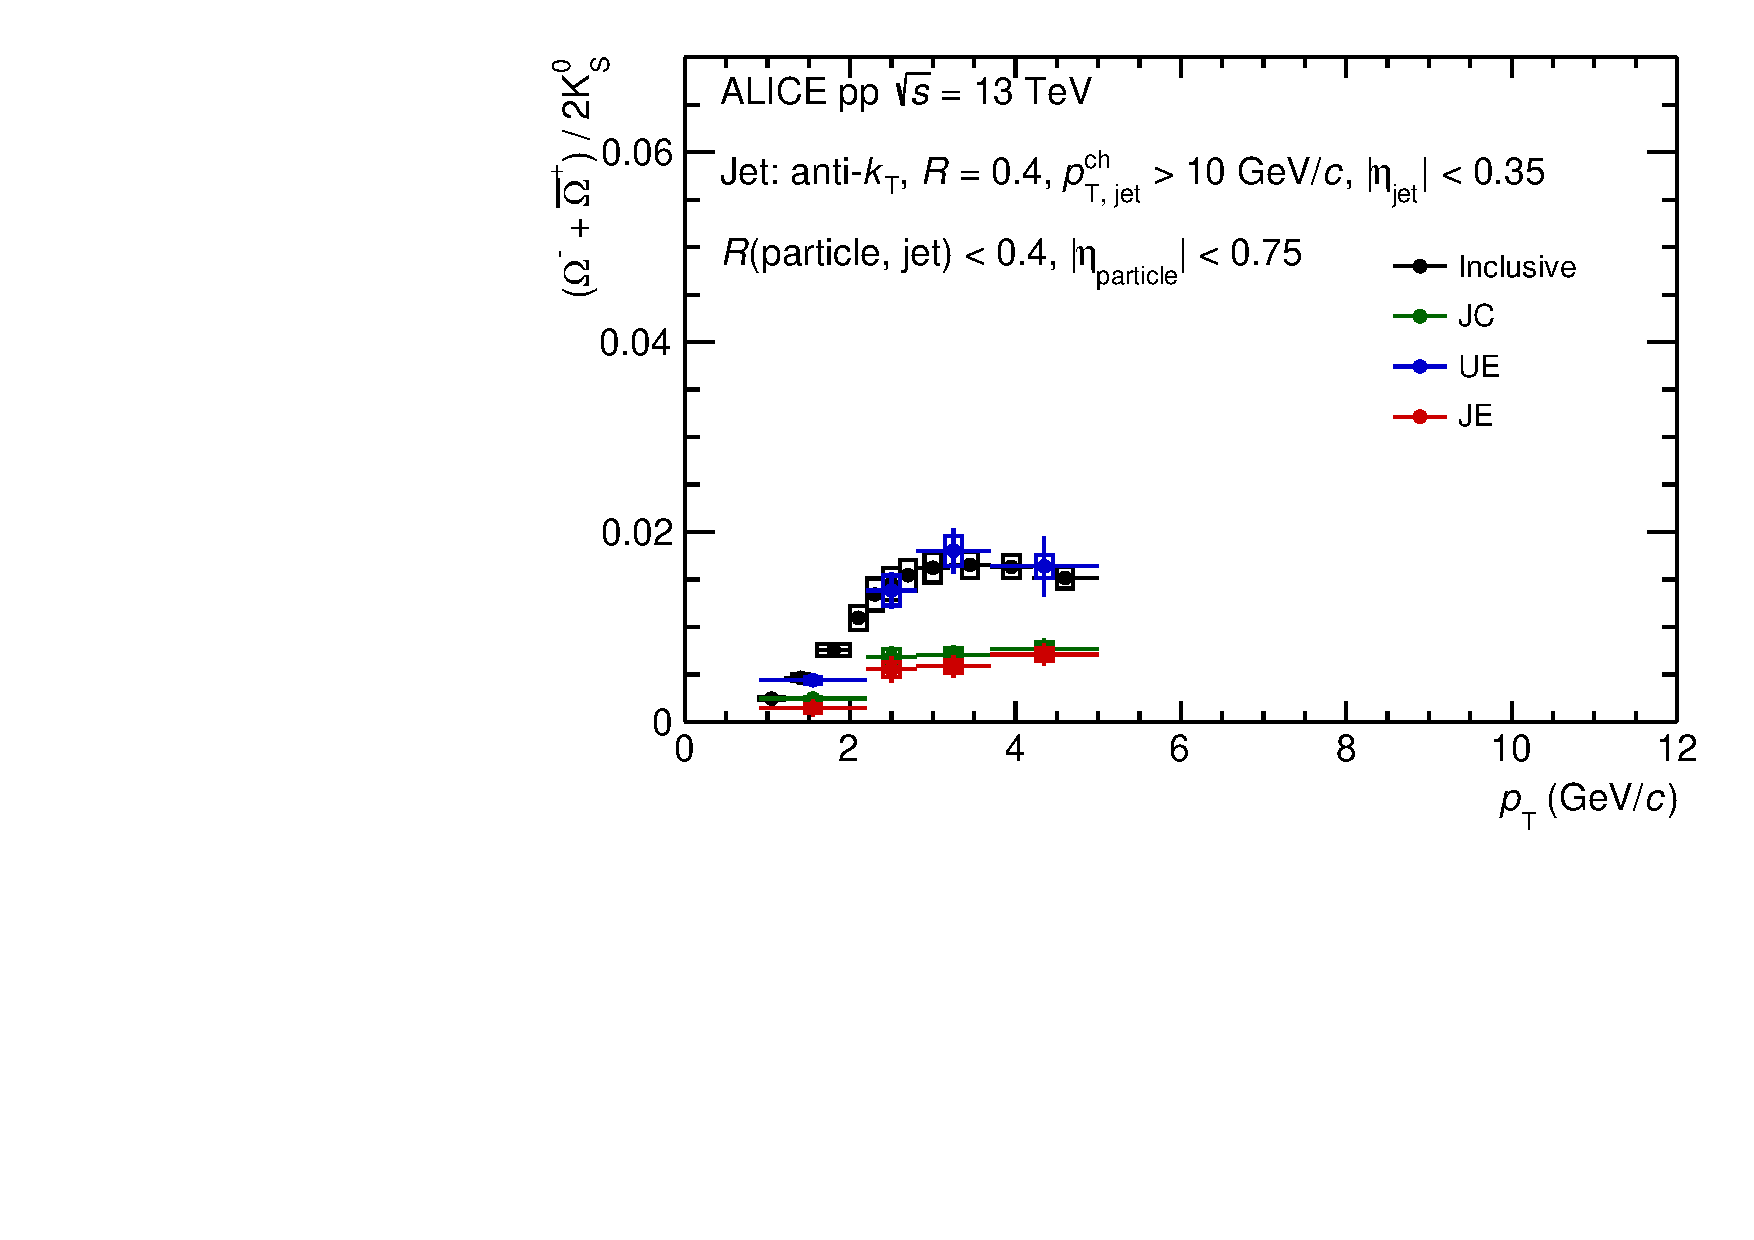
\includegraphics[width=.3\textwidth]{cf07_3}
		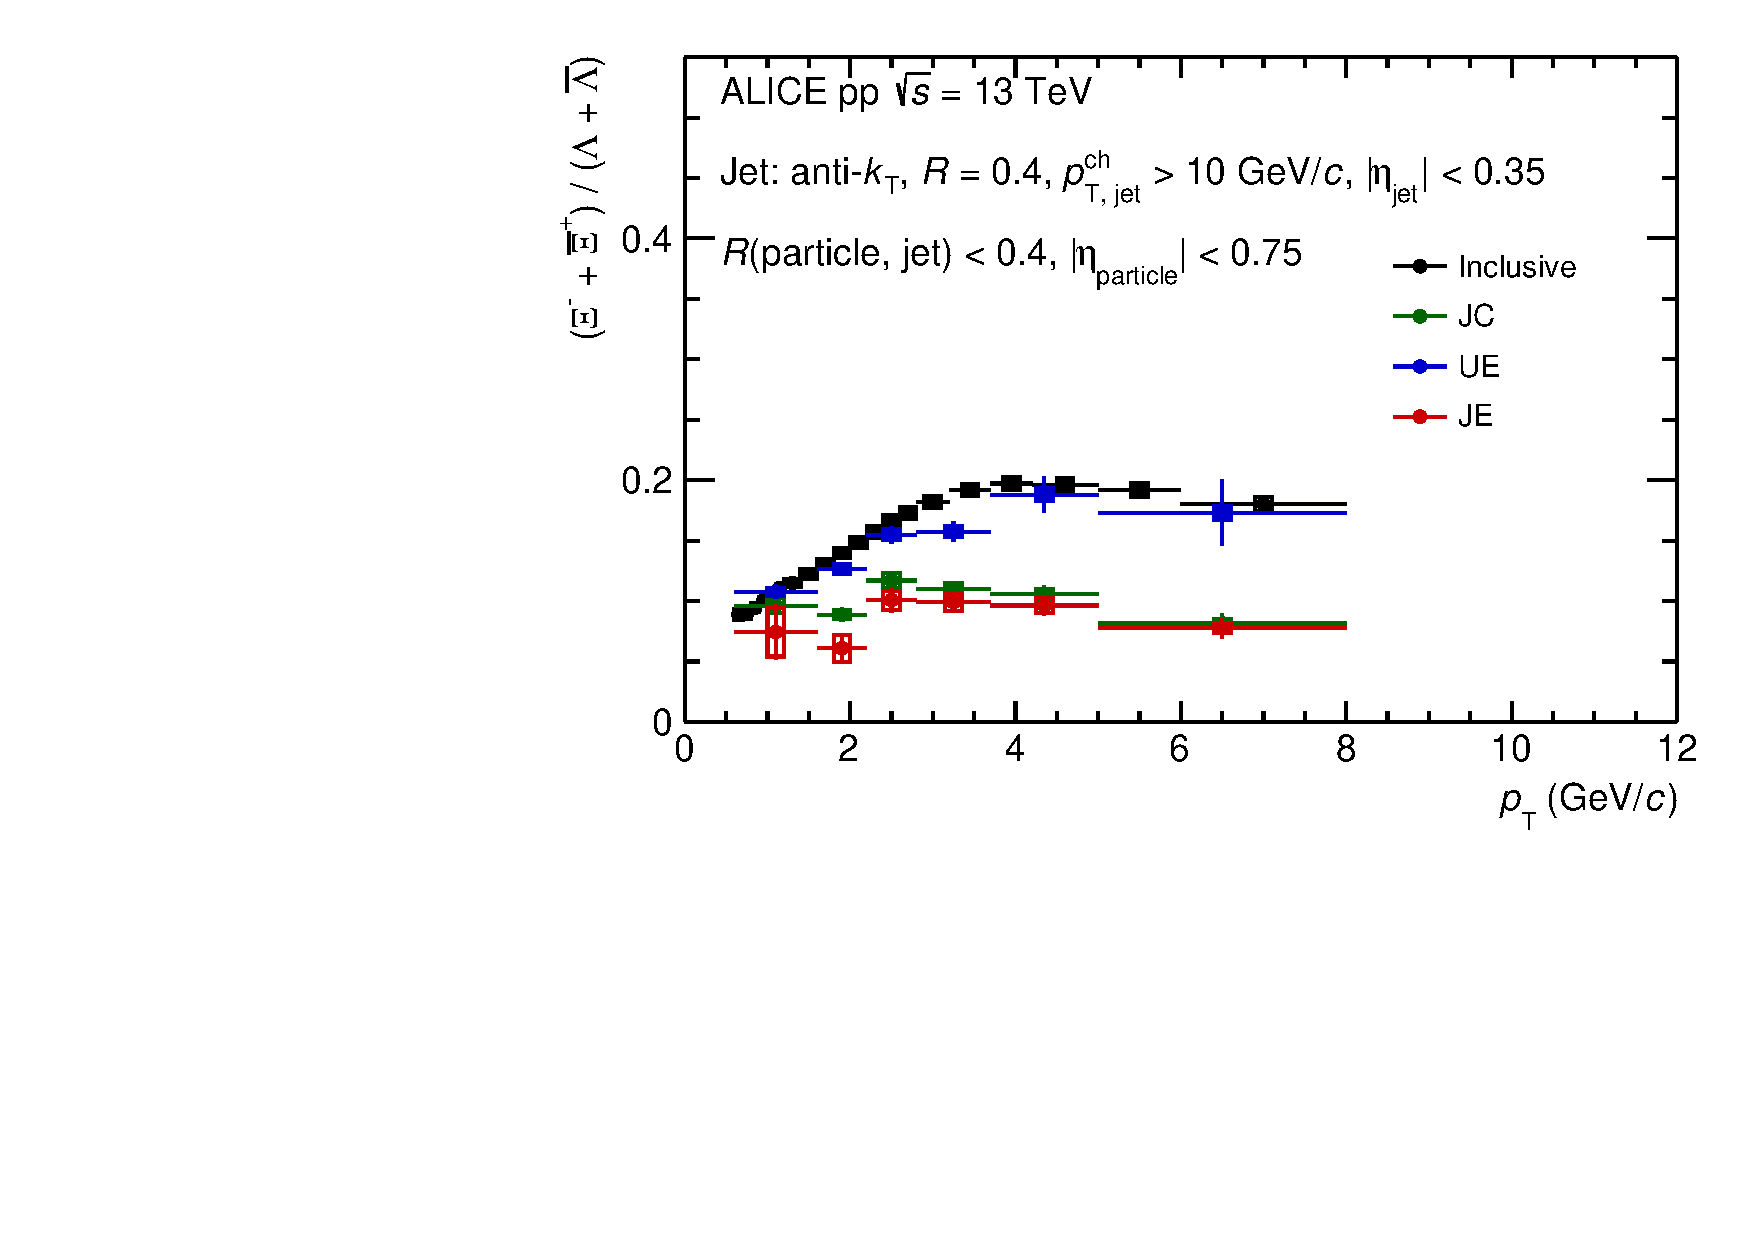
\includegraphics[width=.3\textwidth]{cf07_4}
		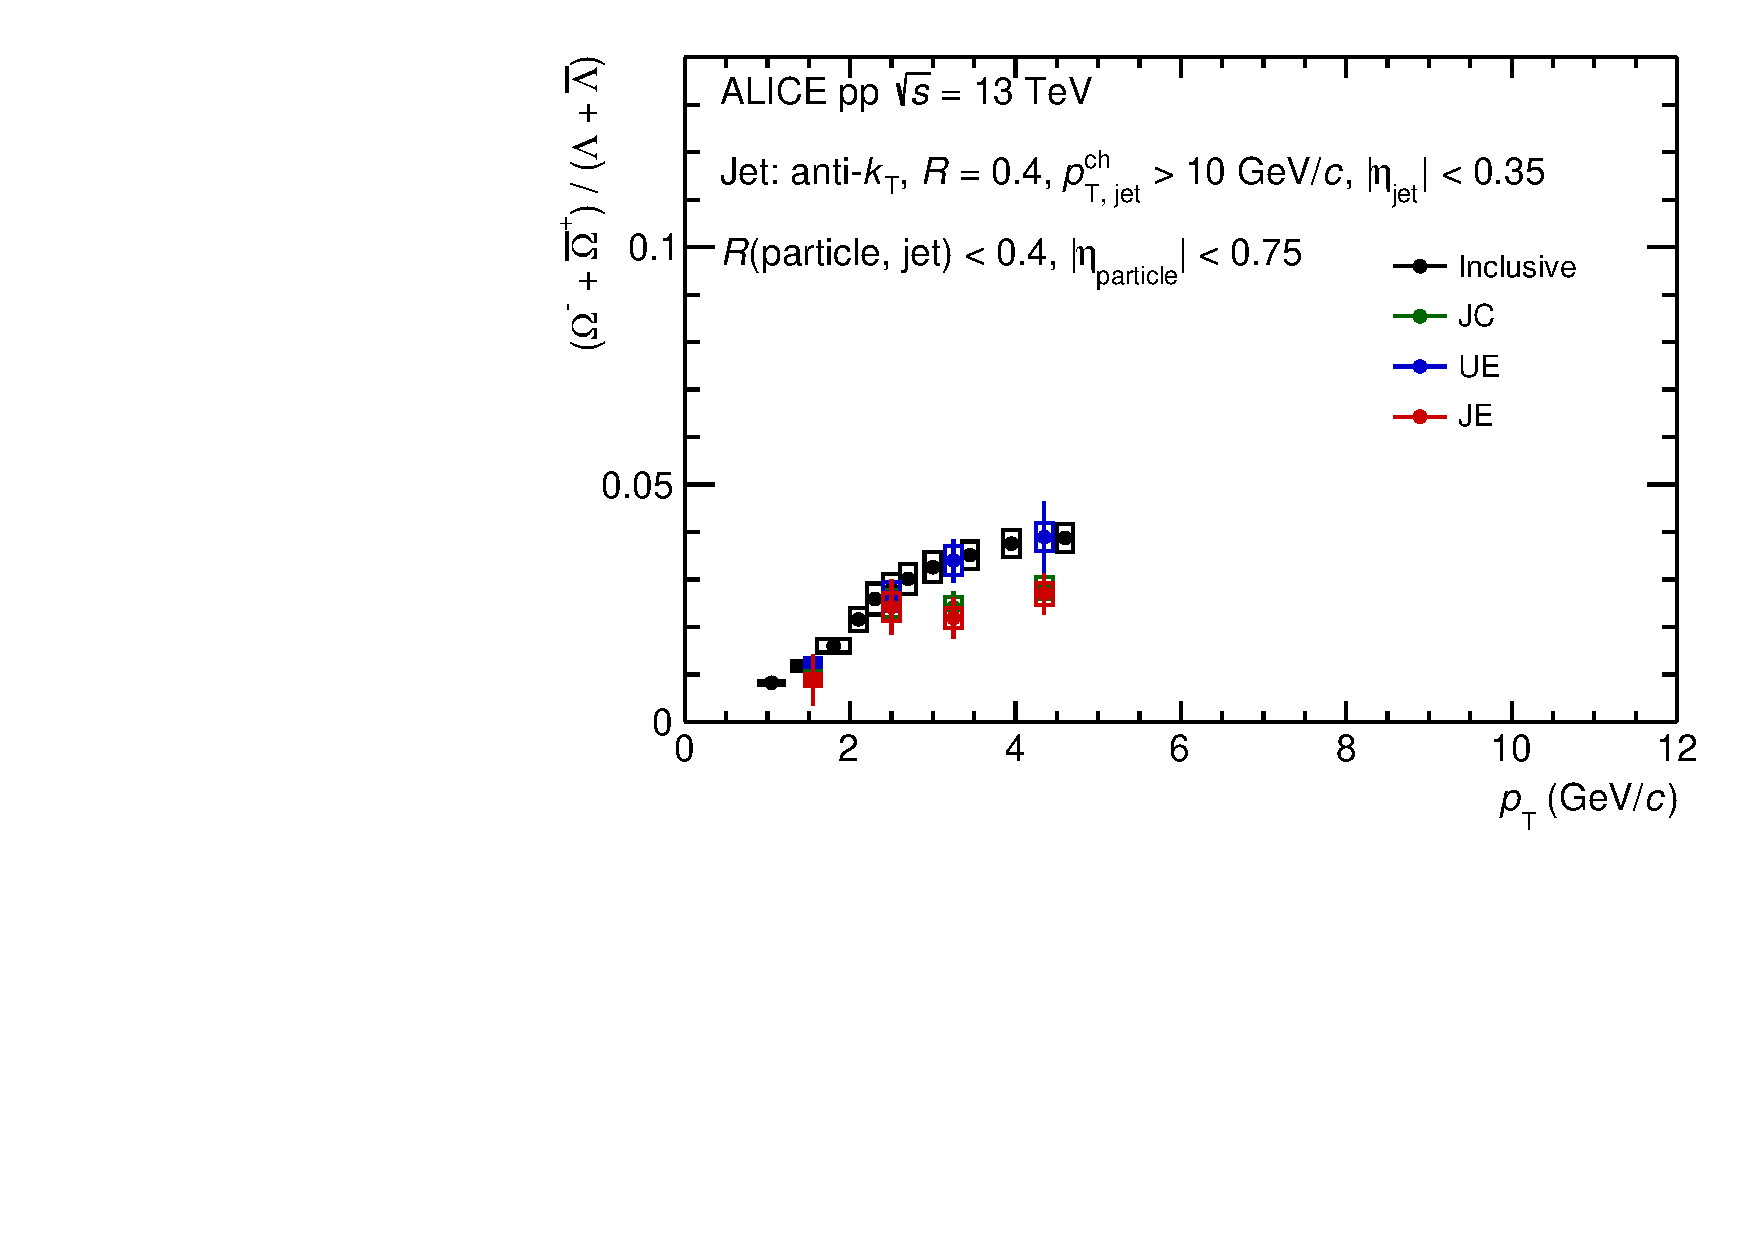
\includegraphics[width=.3\textwidth]{cf07_5}
		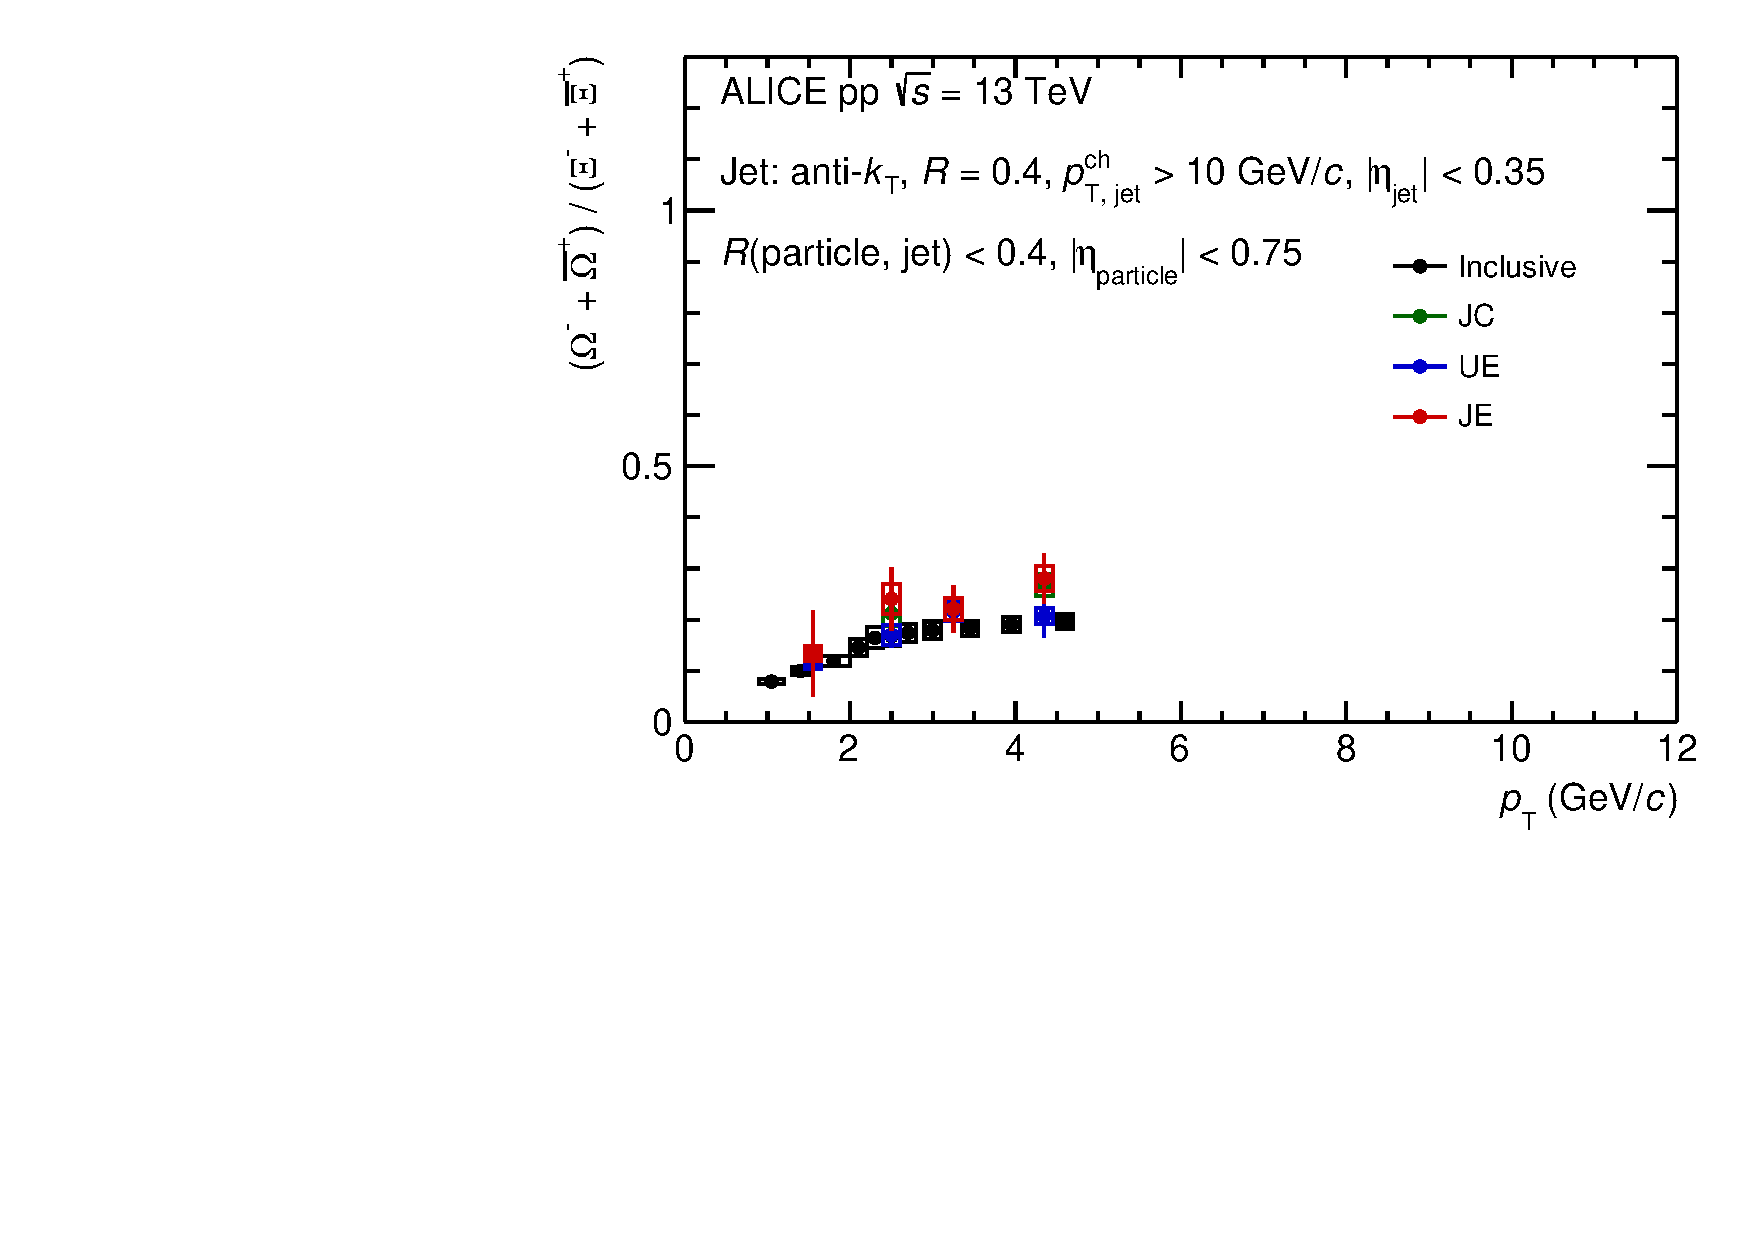
\includegraphics[width=.3\textwidth]{cf07_6}
	\end{center}
	\caption{The baryon-to-meson (top) and baryon-to-baryon(bottom) ratio as a function of particle $\pT$ in \pp collisions at \thirteen. In those panels, the black point shows the ratio with particles from minimum bias events, the green point shows the ratio with particles from the jet cones, the blue point shows the ratio with particles from perpendicular cones with jet and the red point shows the ratio with particles that generated by jet.}
	\label{fig:ppRatio}
\end{figure}
\begin{figure}[!ht]
	\begin{center}
		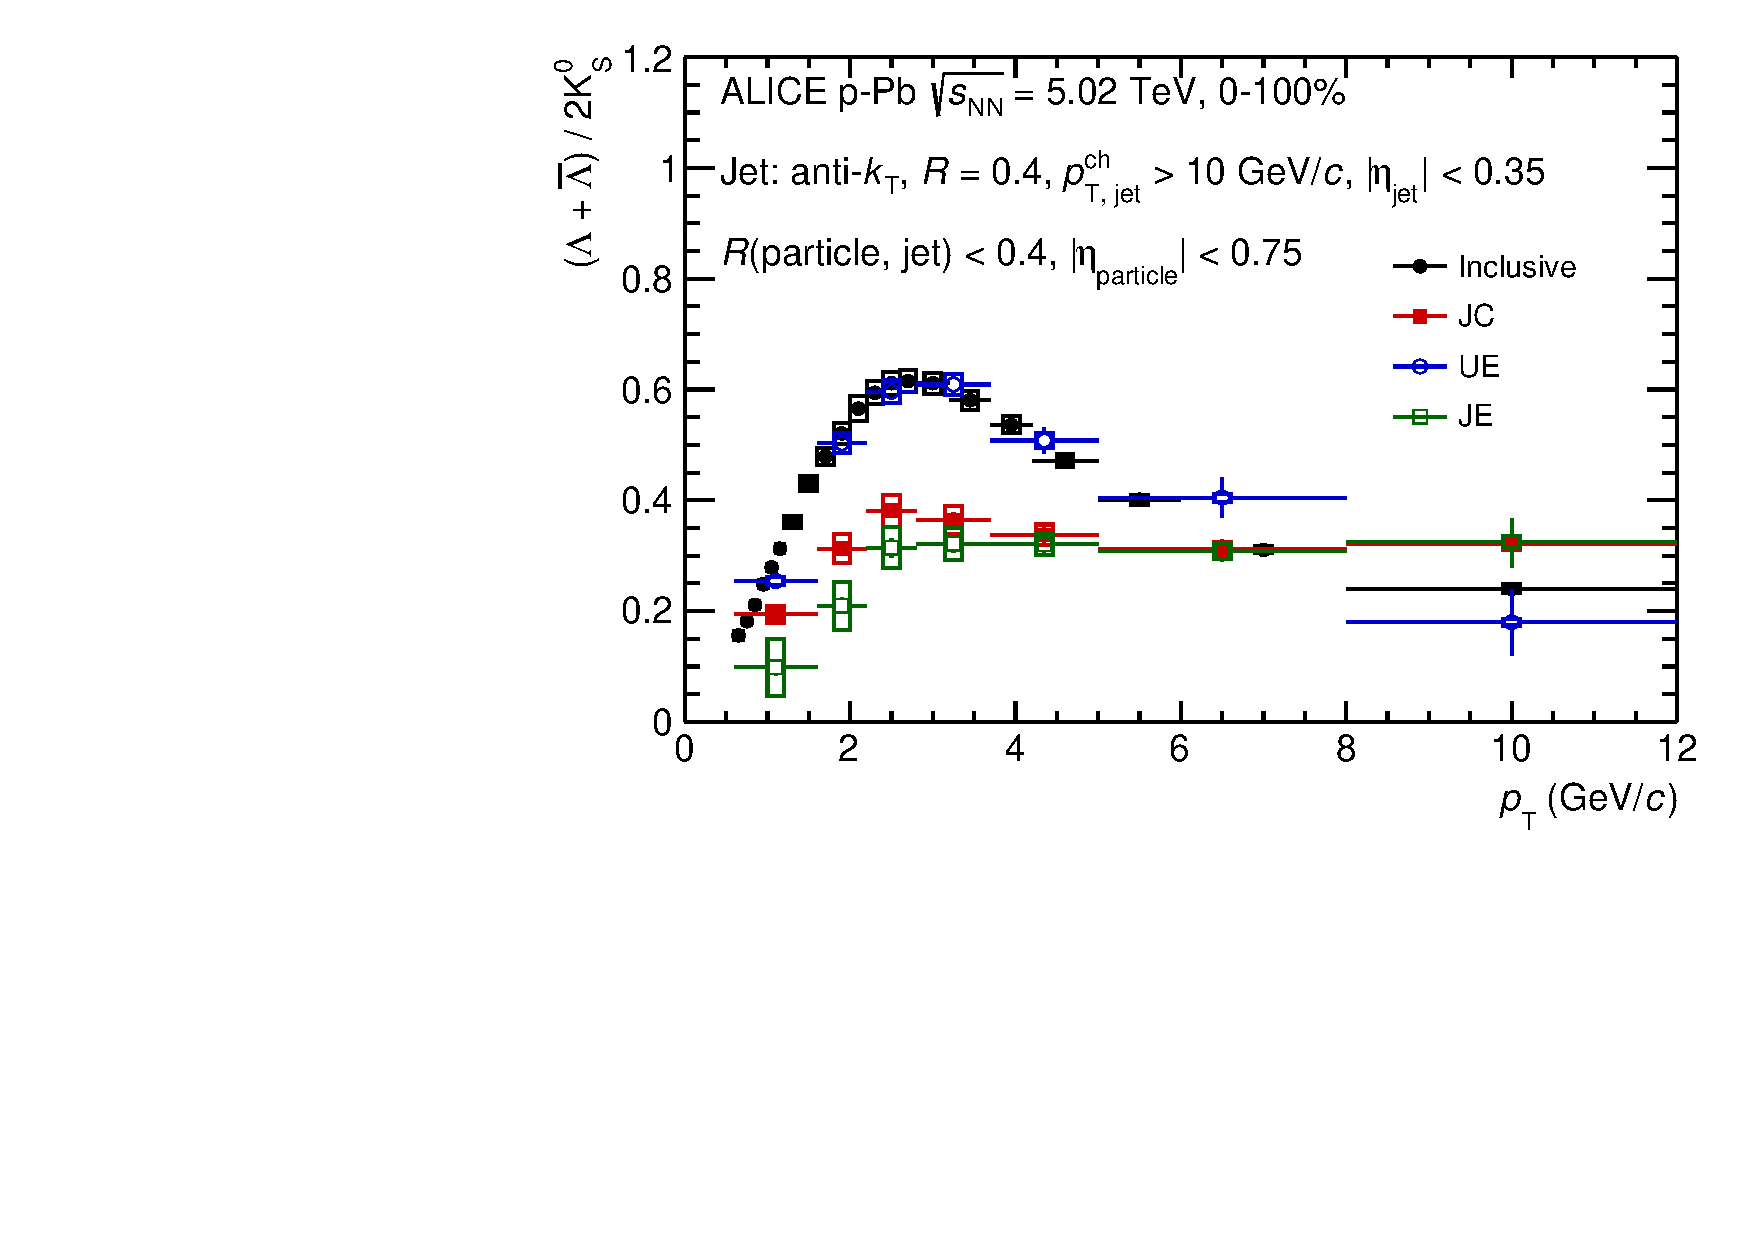
\includegraphics[width=.3\textwidth]{cf08_1}
		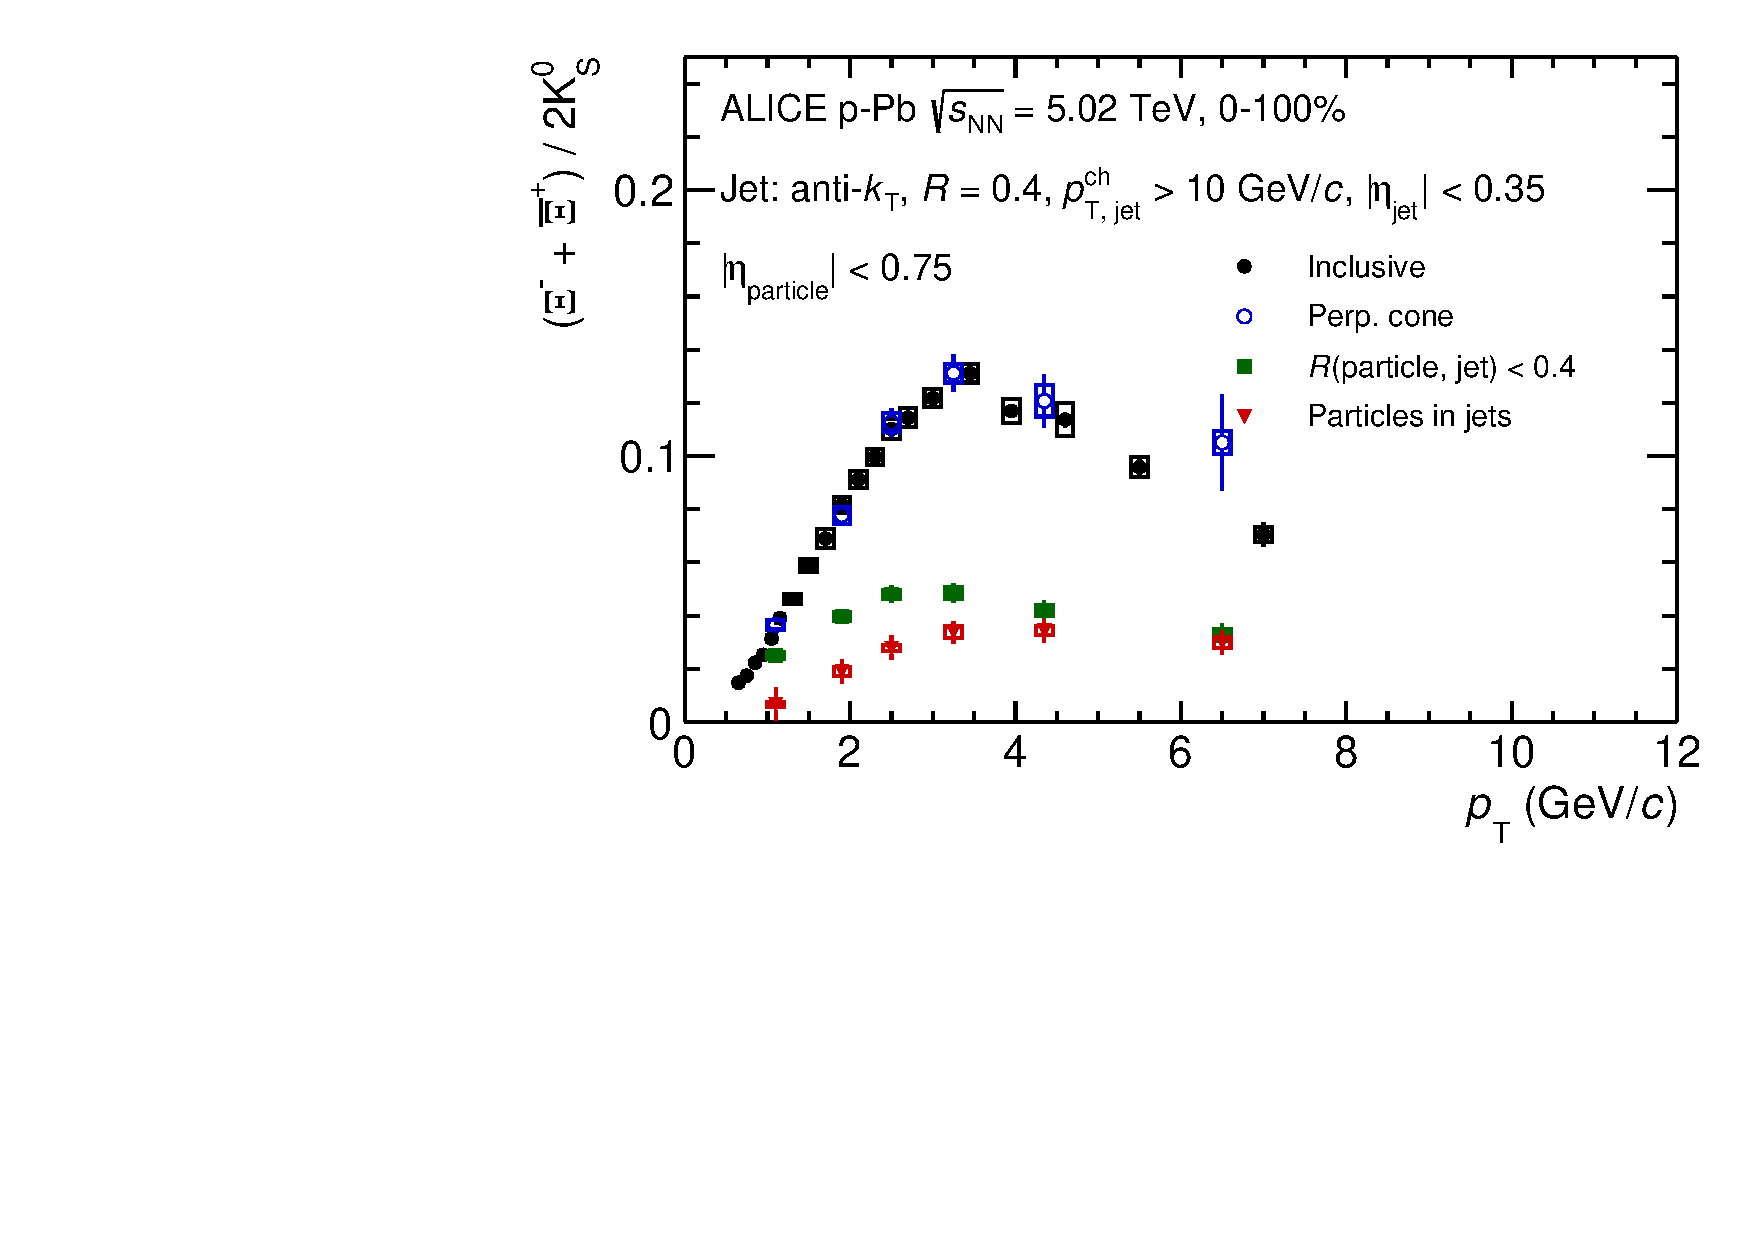
\includegraphics[width=.3\textwidth]{cf08_2}
		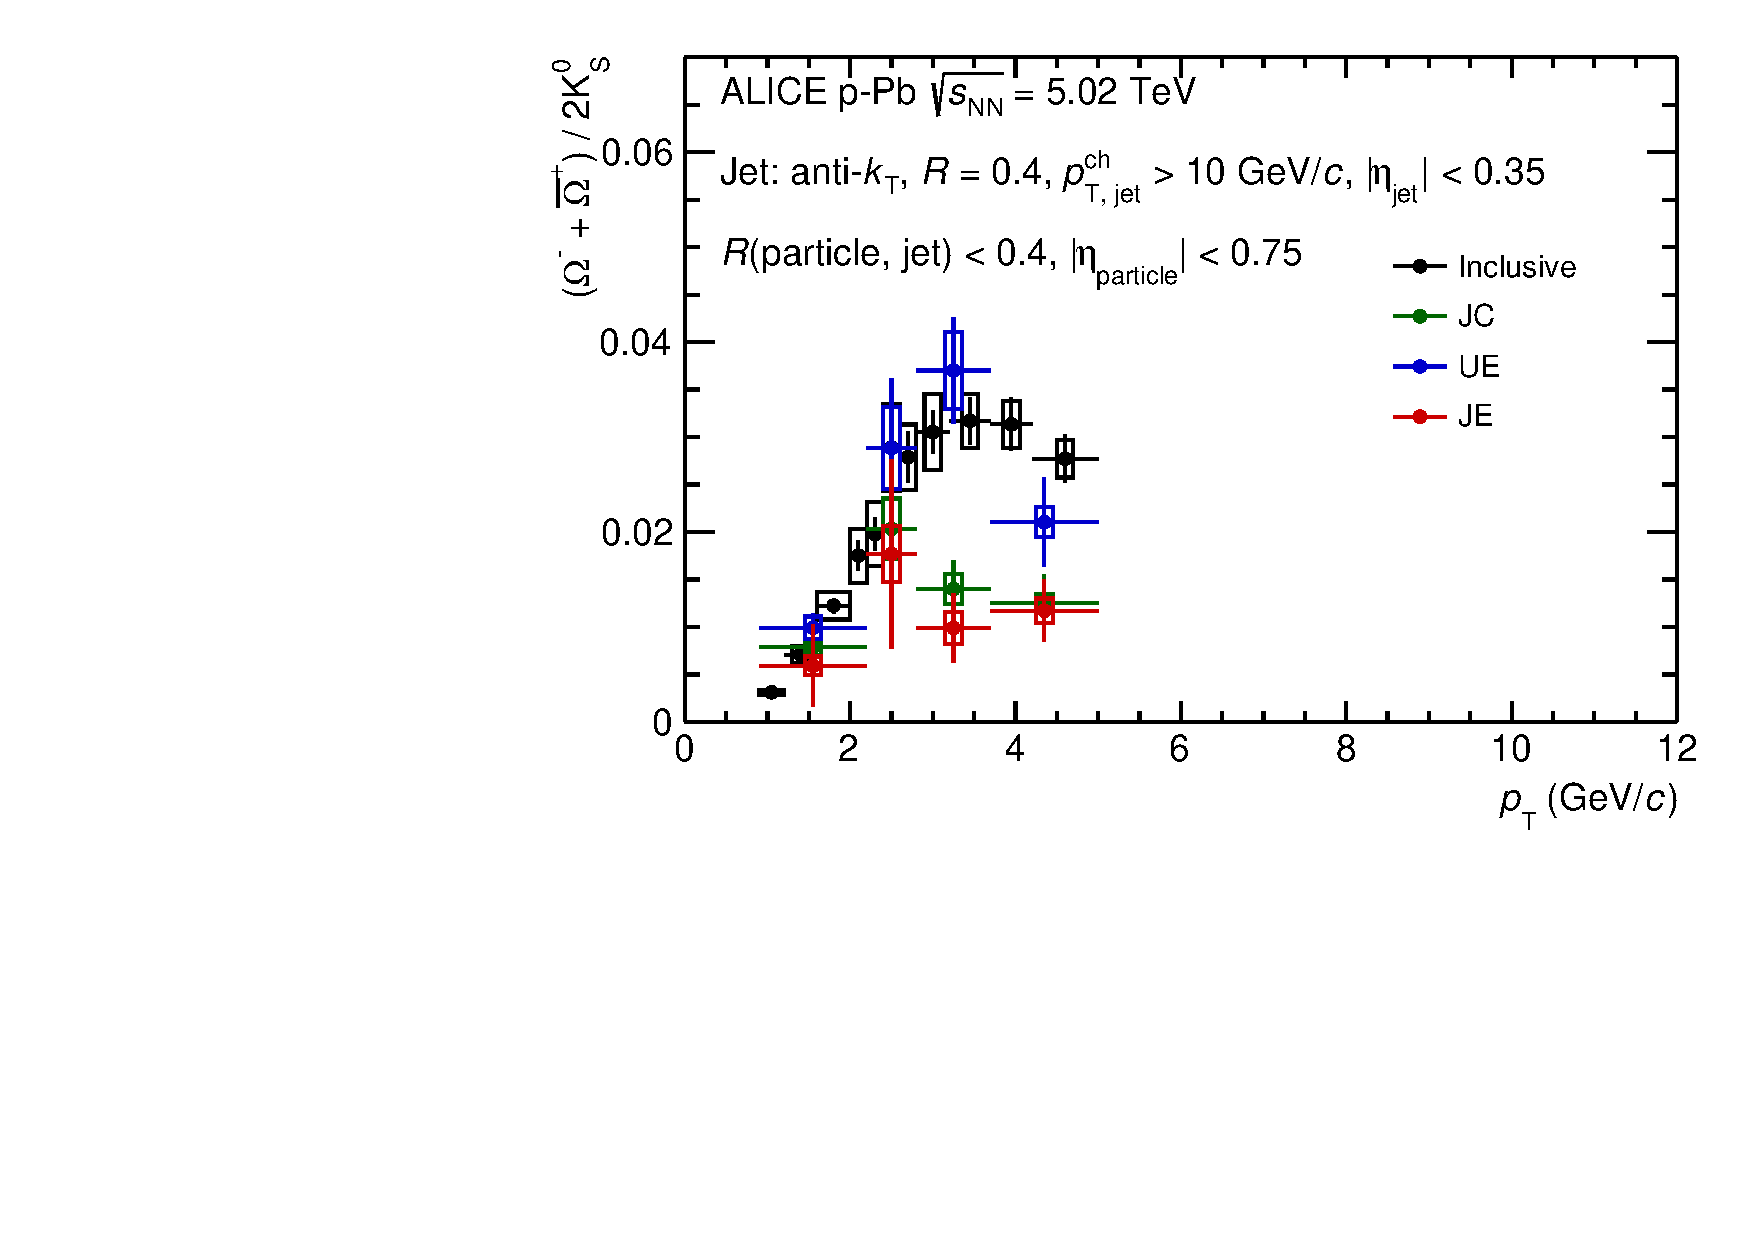
\includegraphics[width=.3\textwidth]{cf08_3}
		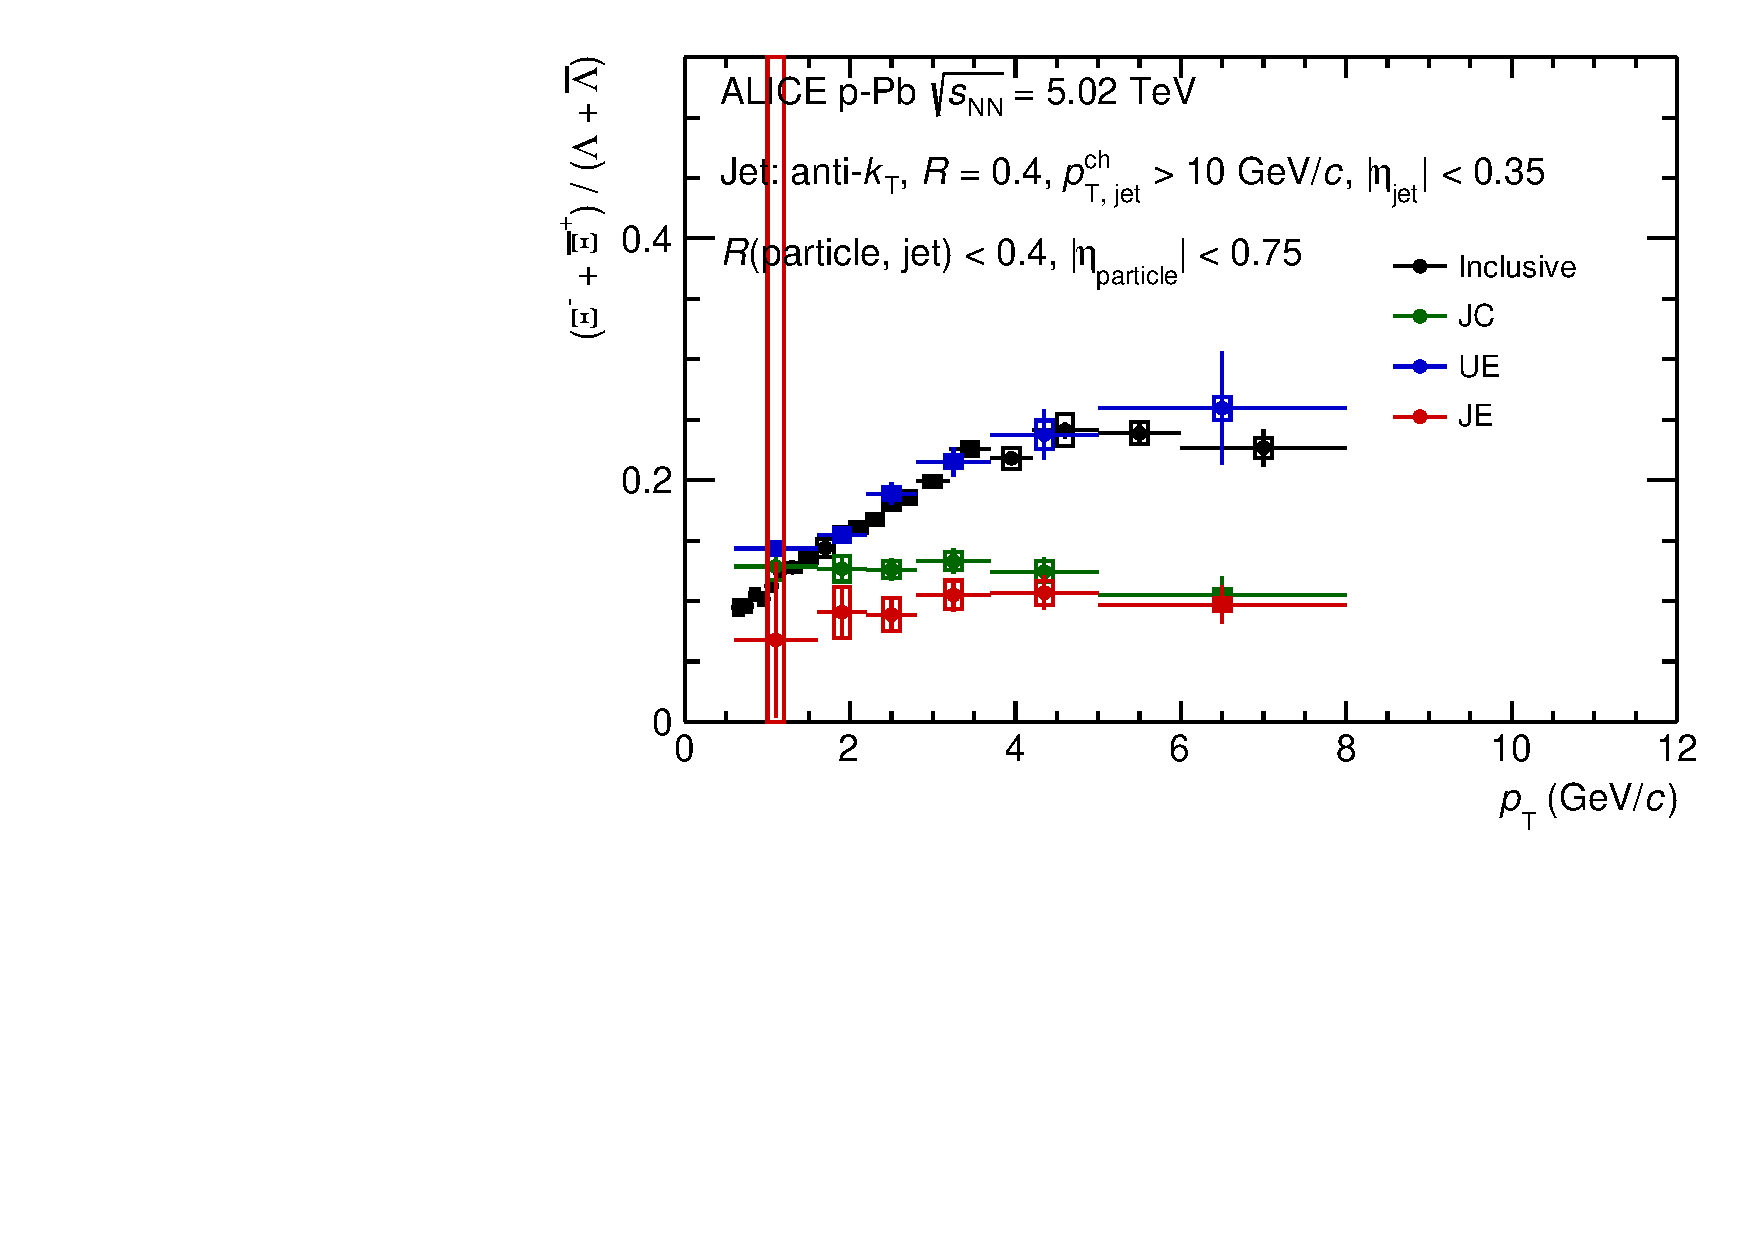
\includegraphics[width=.3\textwidth]{cf08_4}
		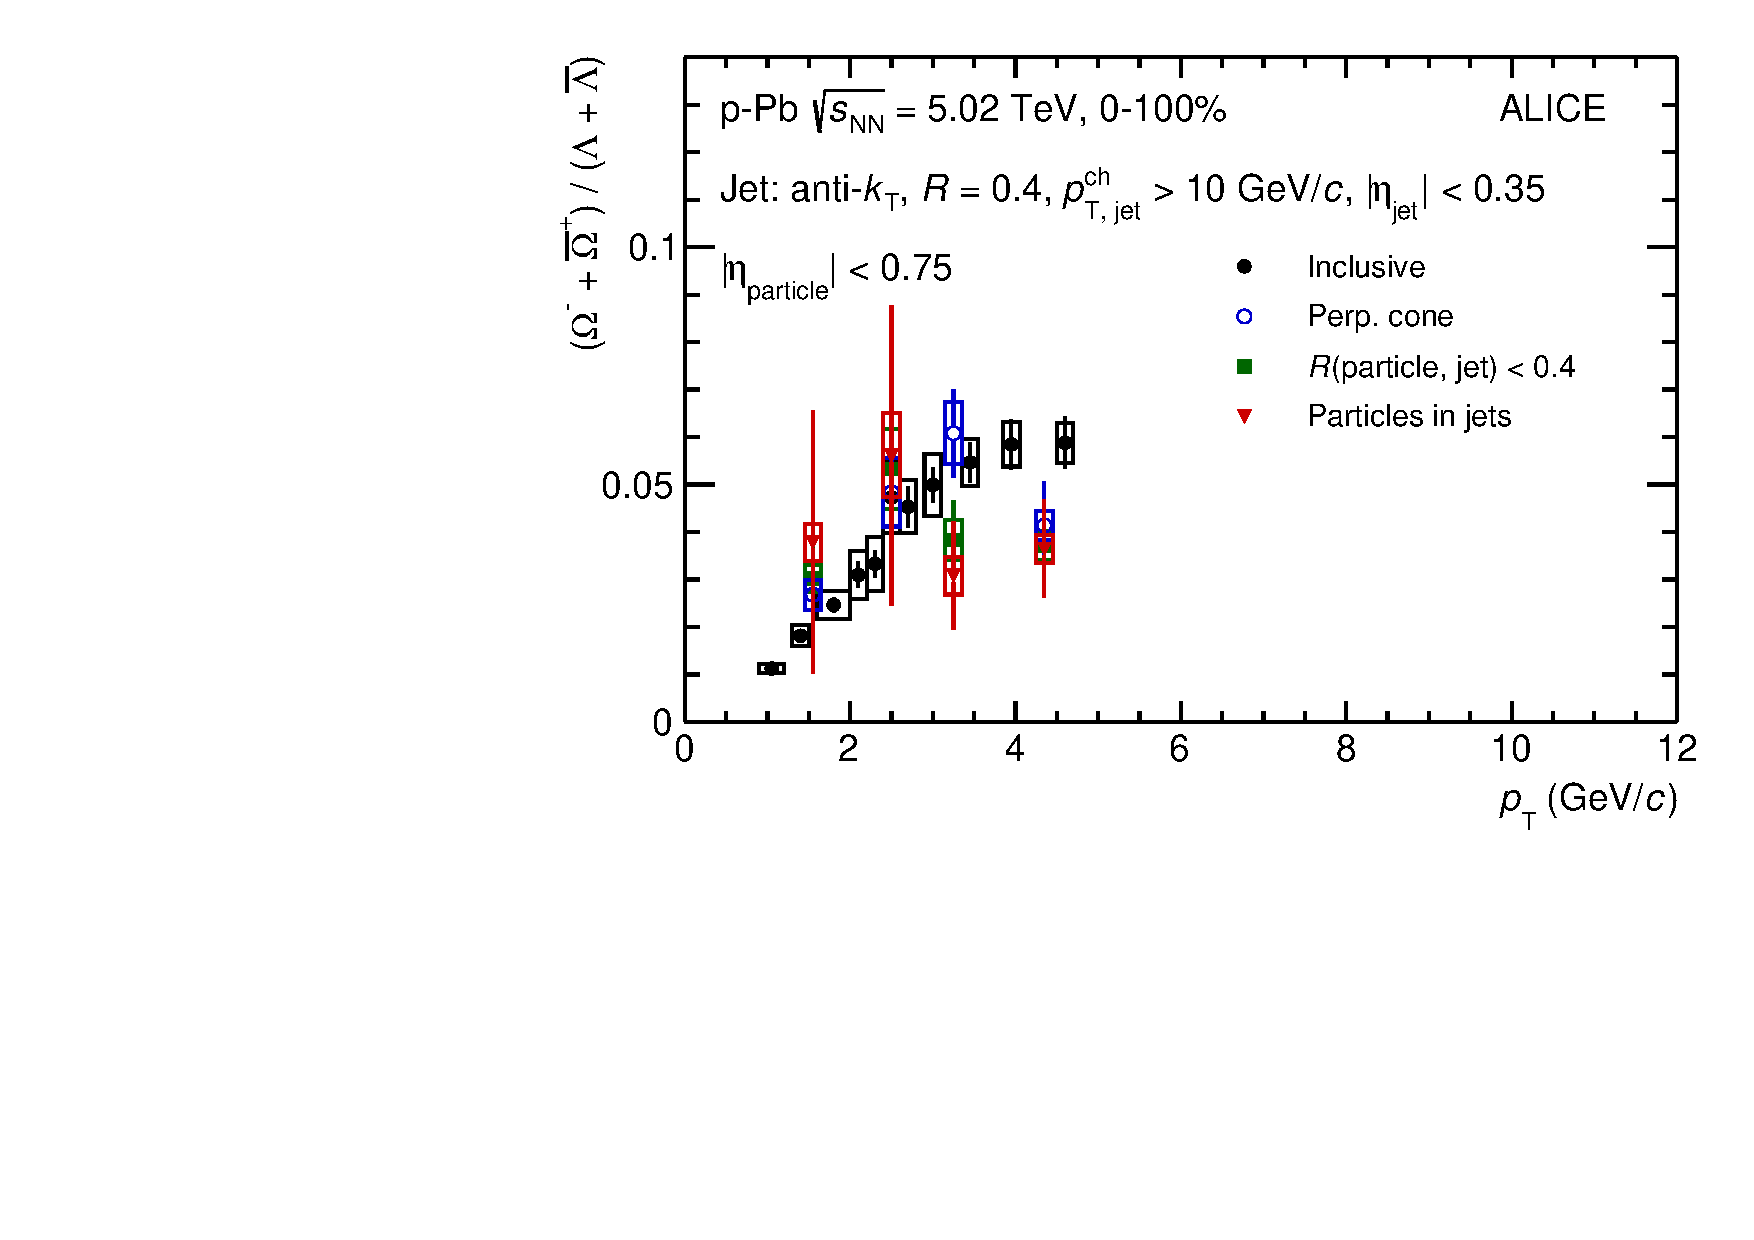
\includegraphics[width=.3\textwidth]{cf08_5}
		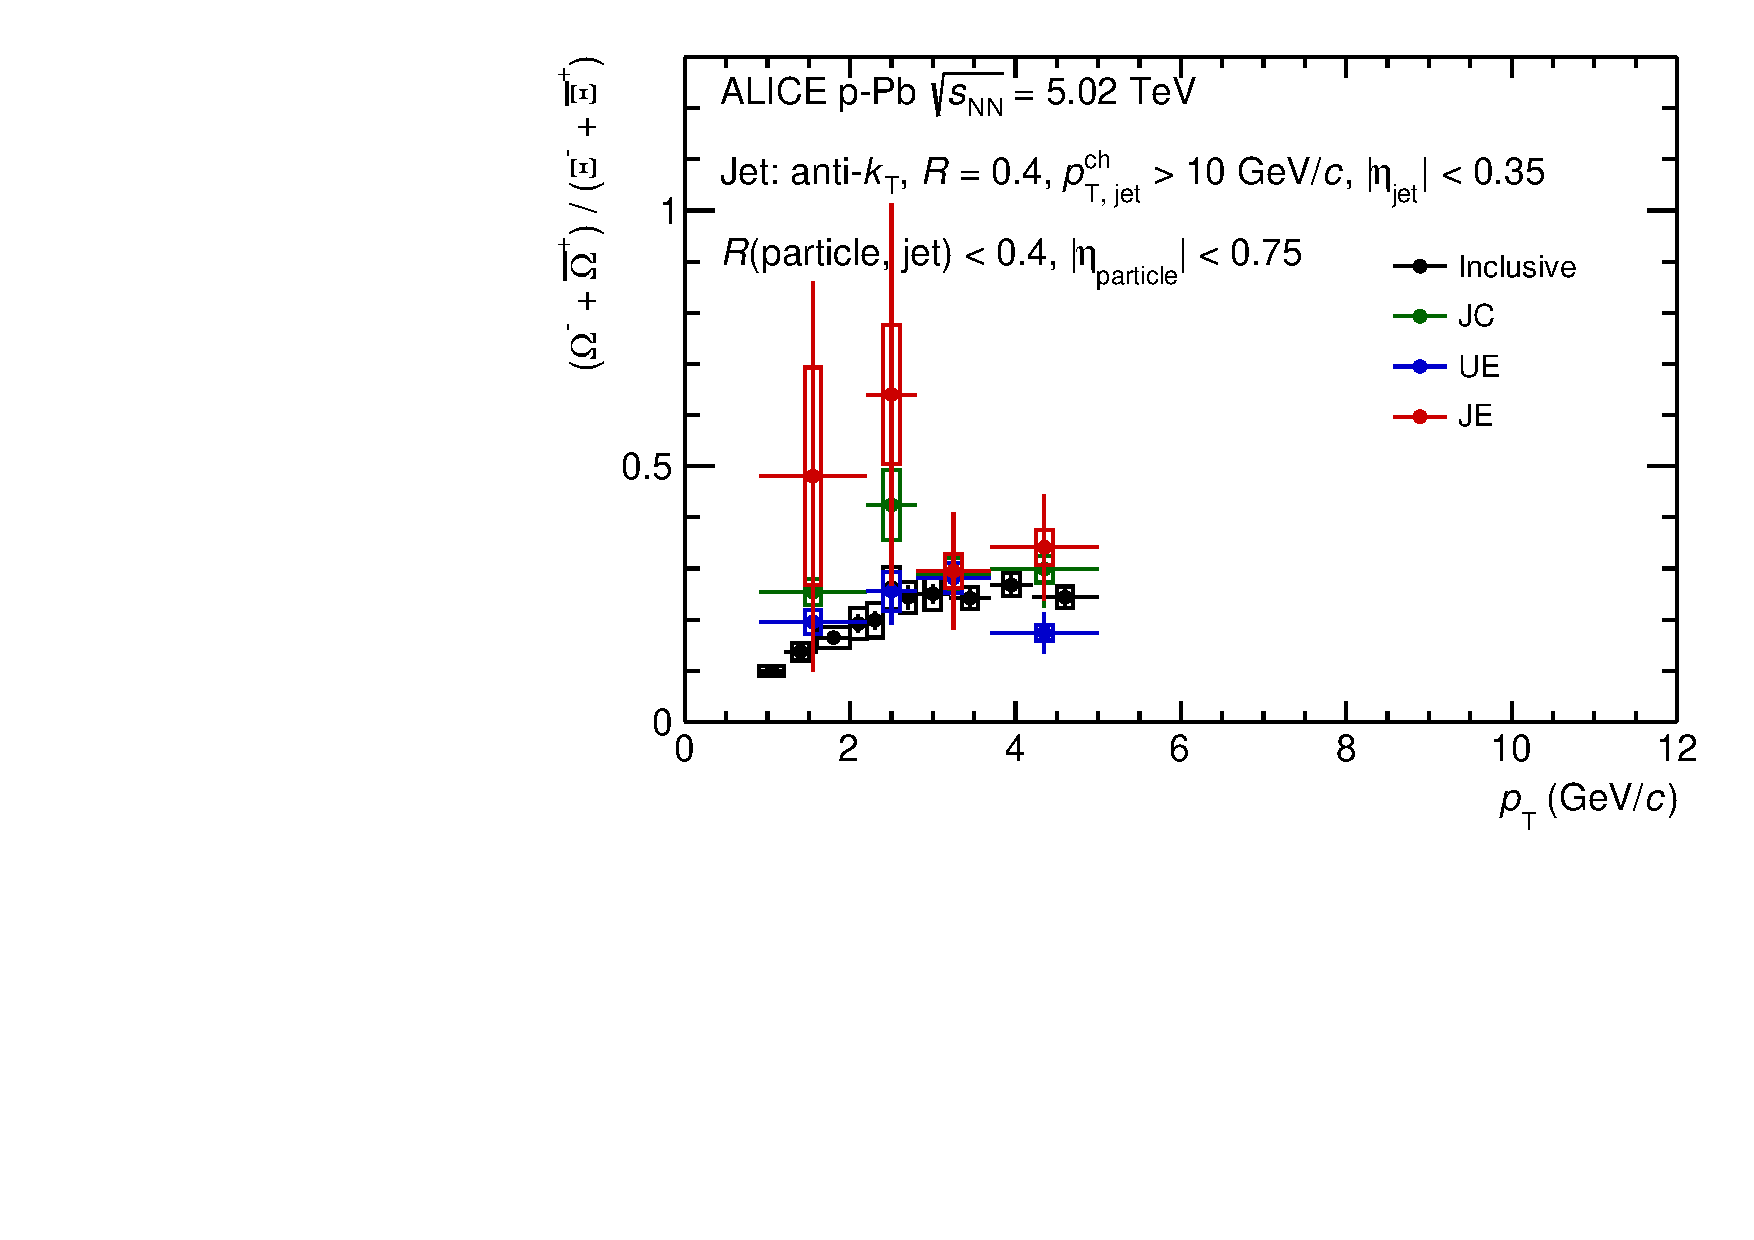
\includegraphics[width=.3\textwidth]{cf08_6}
	\end{center}
	\caption{The baryon-to-meson (top) and baryon-to-baryon(bottom) ratio as a function of particle $\pT$ in \pPb collisions at \fivenn. In those panels, the black point shows the ratio with particles from minimum bias events, the green point shows the ratio with particles from the jet cones, the blue point shows the ratio with particles from perpendicular cones with jet and the red point shows the ratio with particles that generated by jet.}
	\label{fig:pPbRatio}
\end{figure}

The particle ratios in jet with centrality and collision system distribution is studied in Fig.~\ref{fig:pppPbRatio}. The particle ratios in the jet are observed to be relatively centrality and system independent. It is noteworthy that the baryon-to-meson ($\lmb/\kzero$, $\Xi/\kzero$ and $\Omega/\kzero$) ratios have a hint of centrality (collision system) dependent for $2 < \pT < 4$~\GeVc, however this is barely significant given the quoted uncertainties. For $\pT > 5$~\GeVc, the baryon-to-meson ratios become fairly consistent for all centrality classes and collision systems. 

\begin{figure}[!ht]
	\begin{center}
		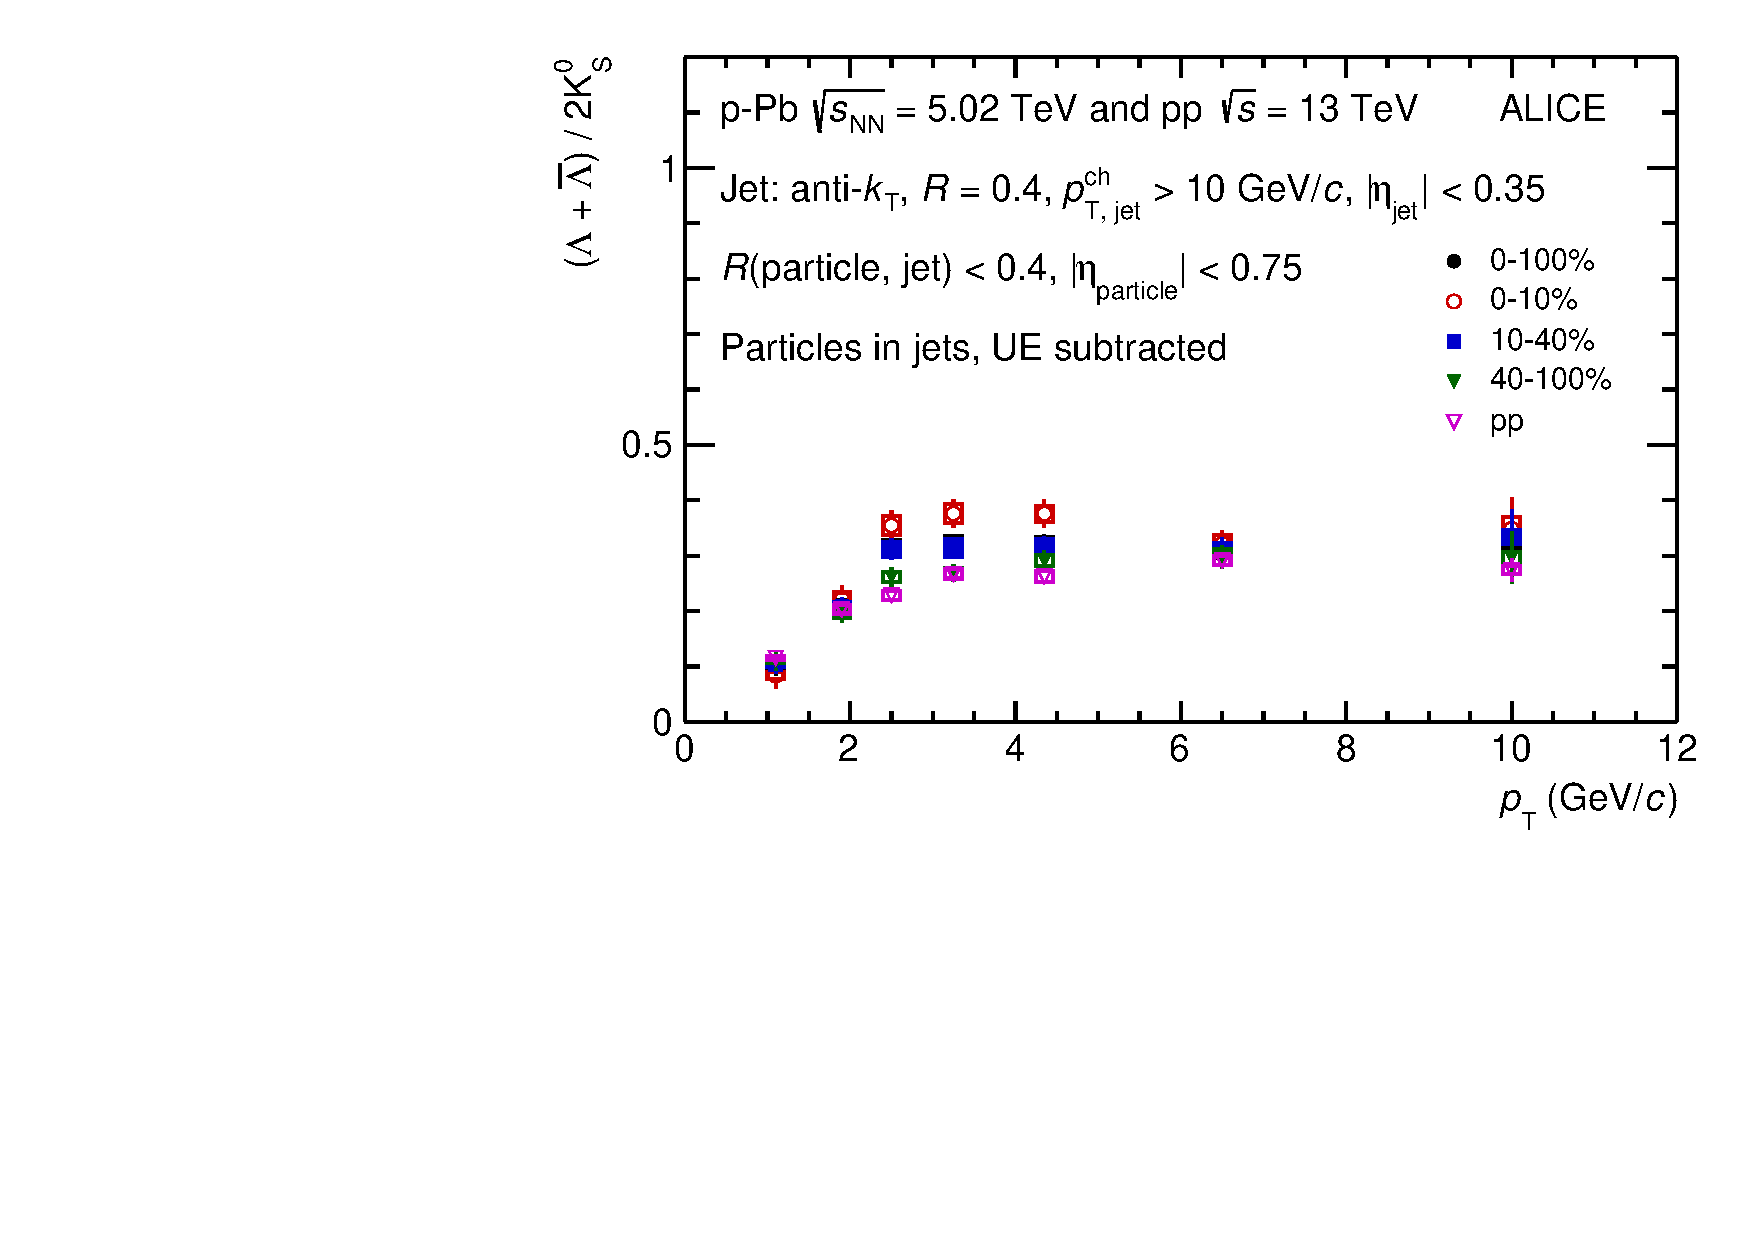
\includegraphics[width=.3\textwidth]{cf09_1}
		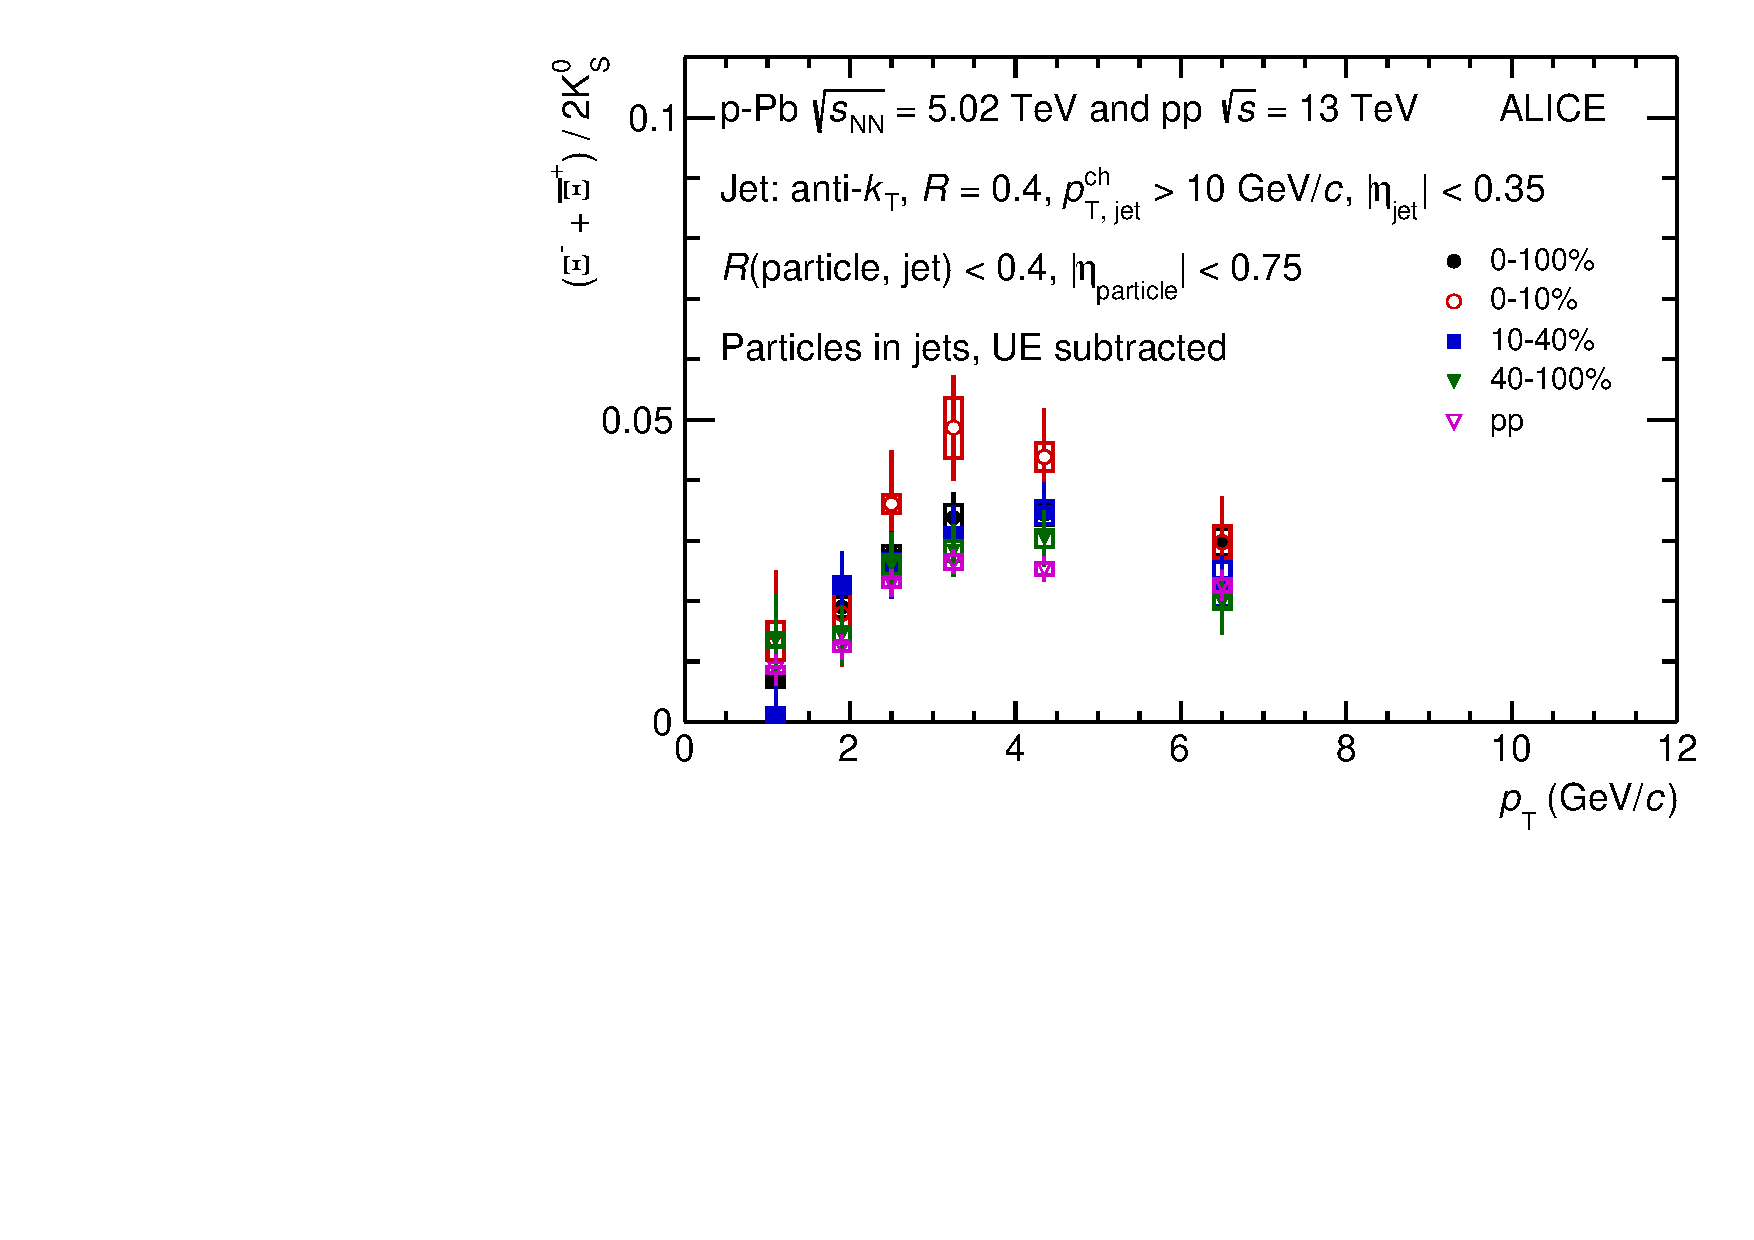
\includegraphics[width=.3\textwidth]{cf09_2}
		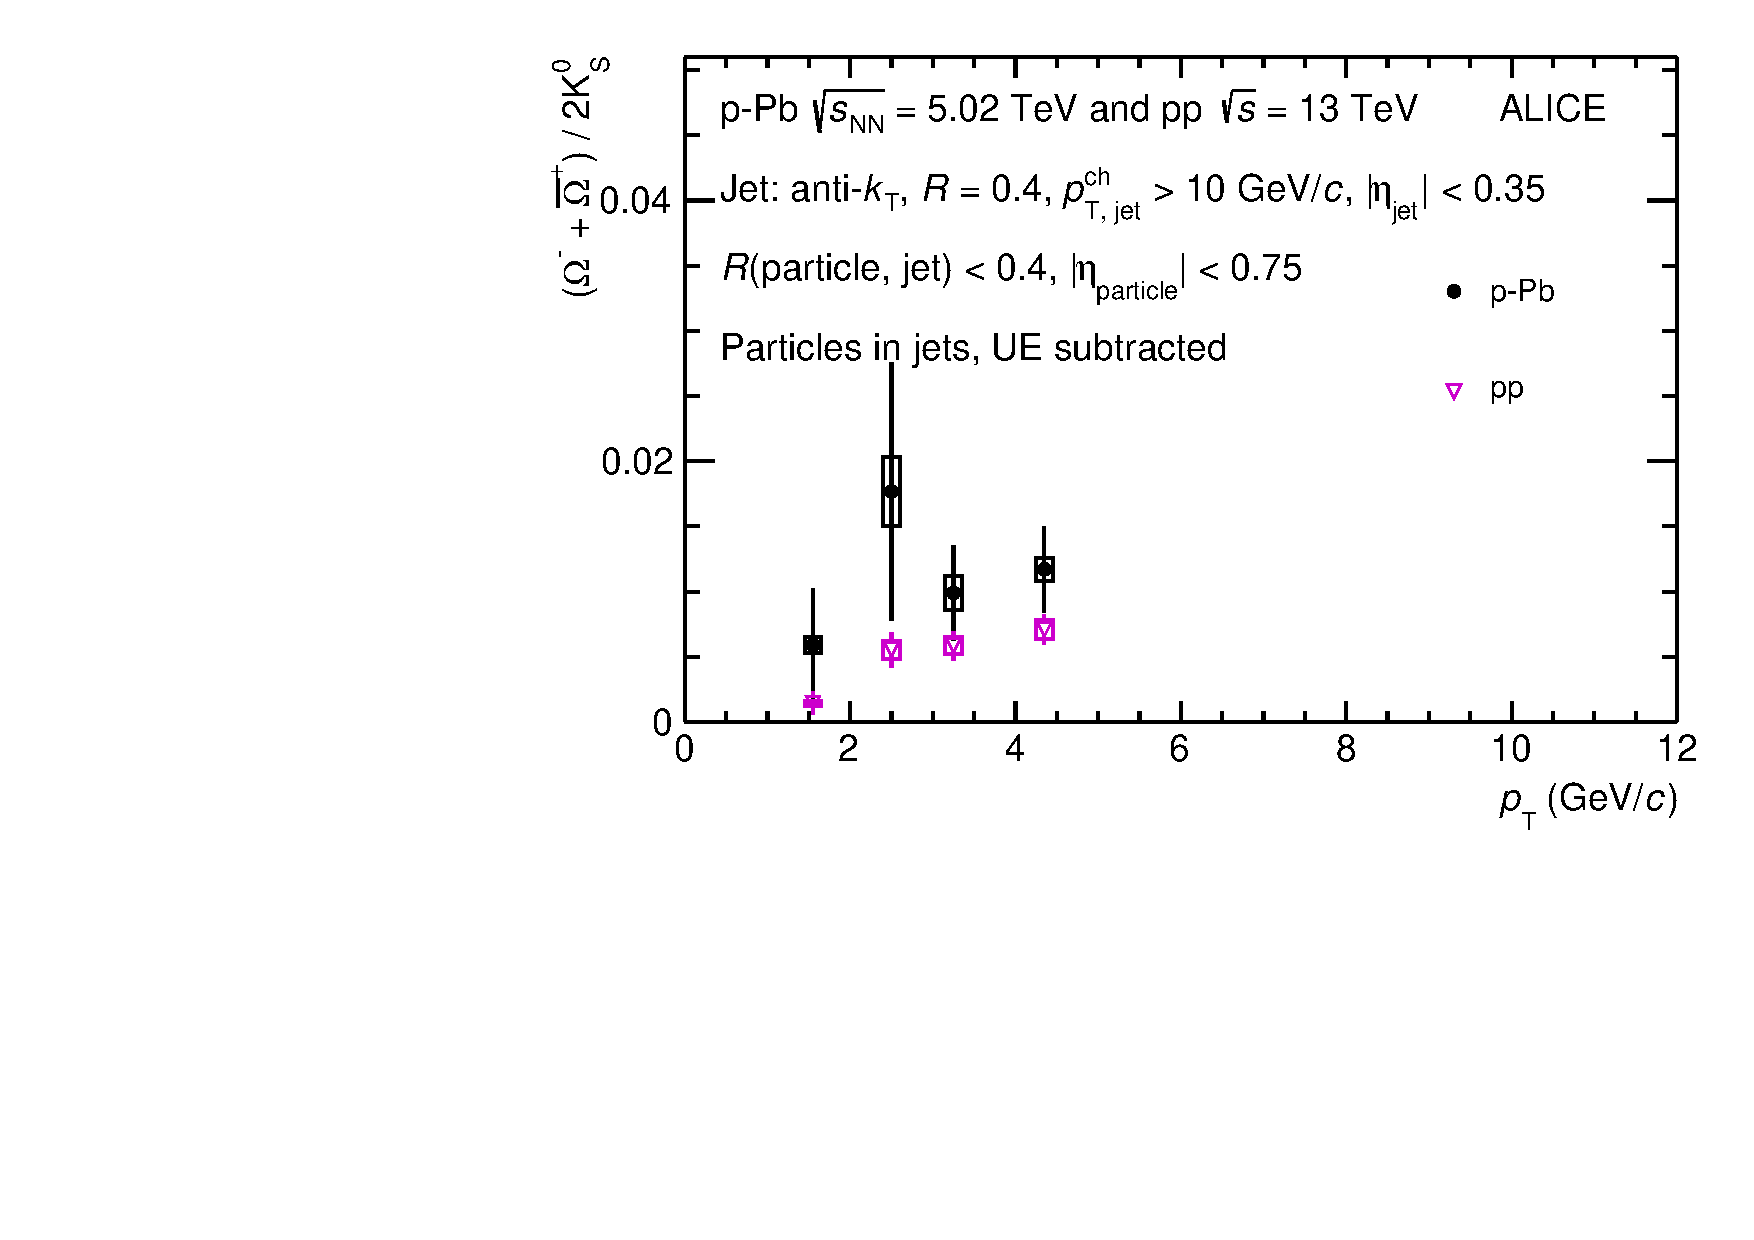
\includegraphics[width=.3\textwidth]{cf09_3}
		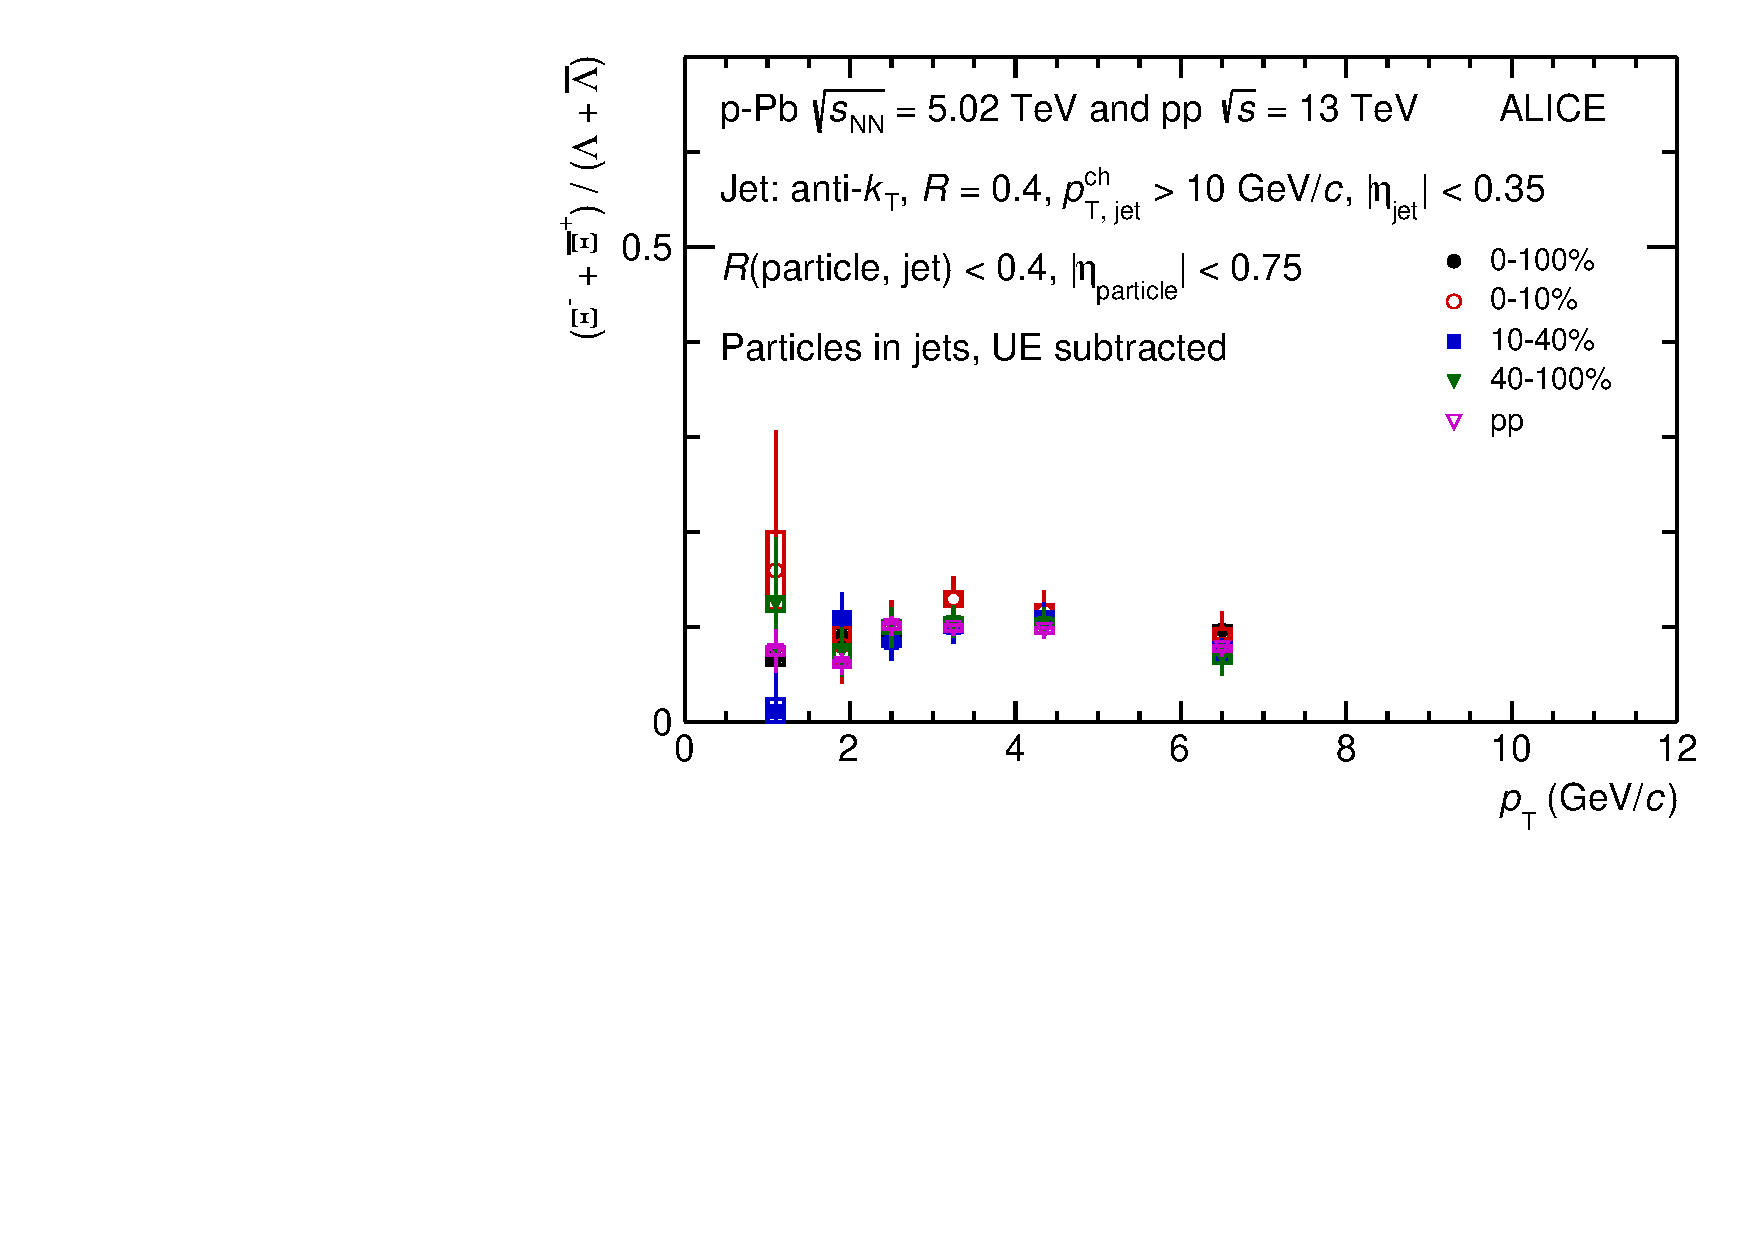
\includegraphics[width=.3\textwidth]{cf09_4}
		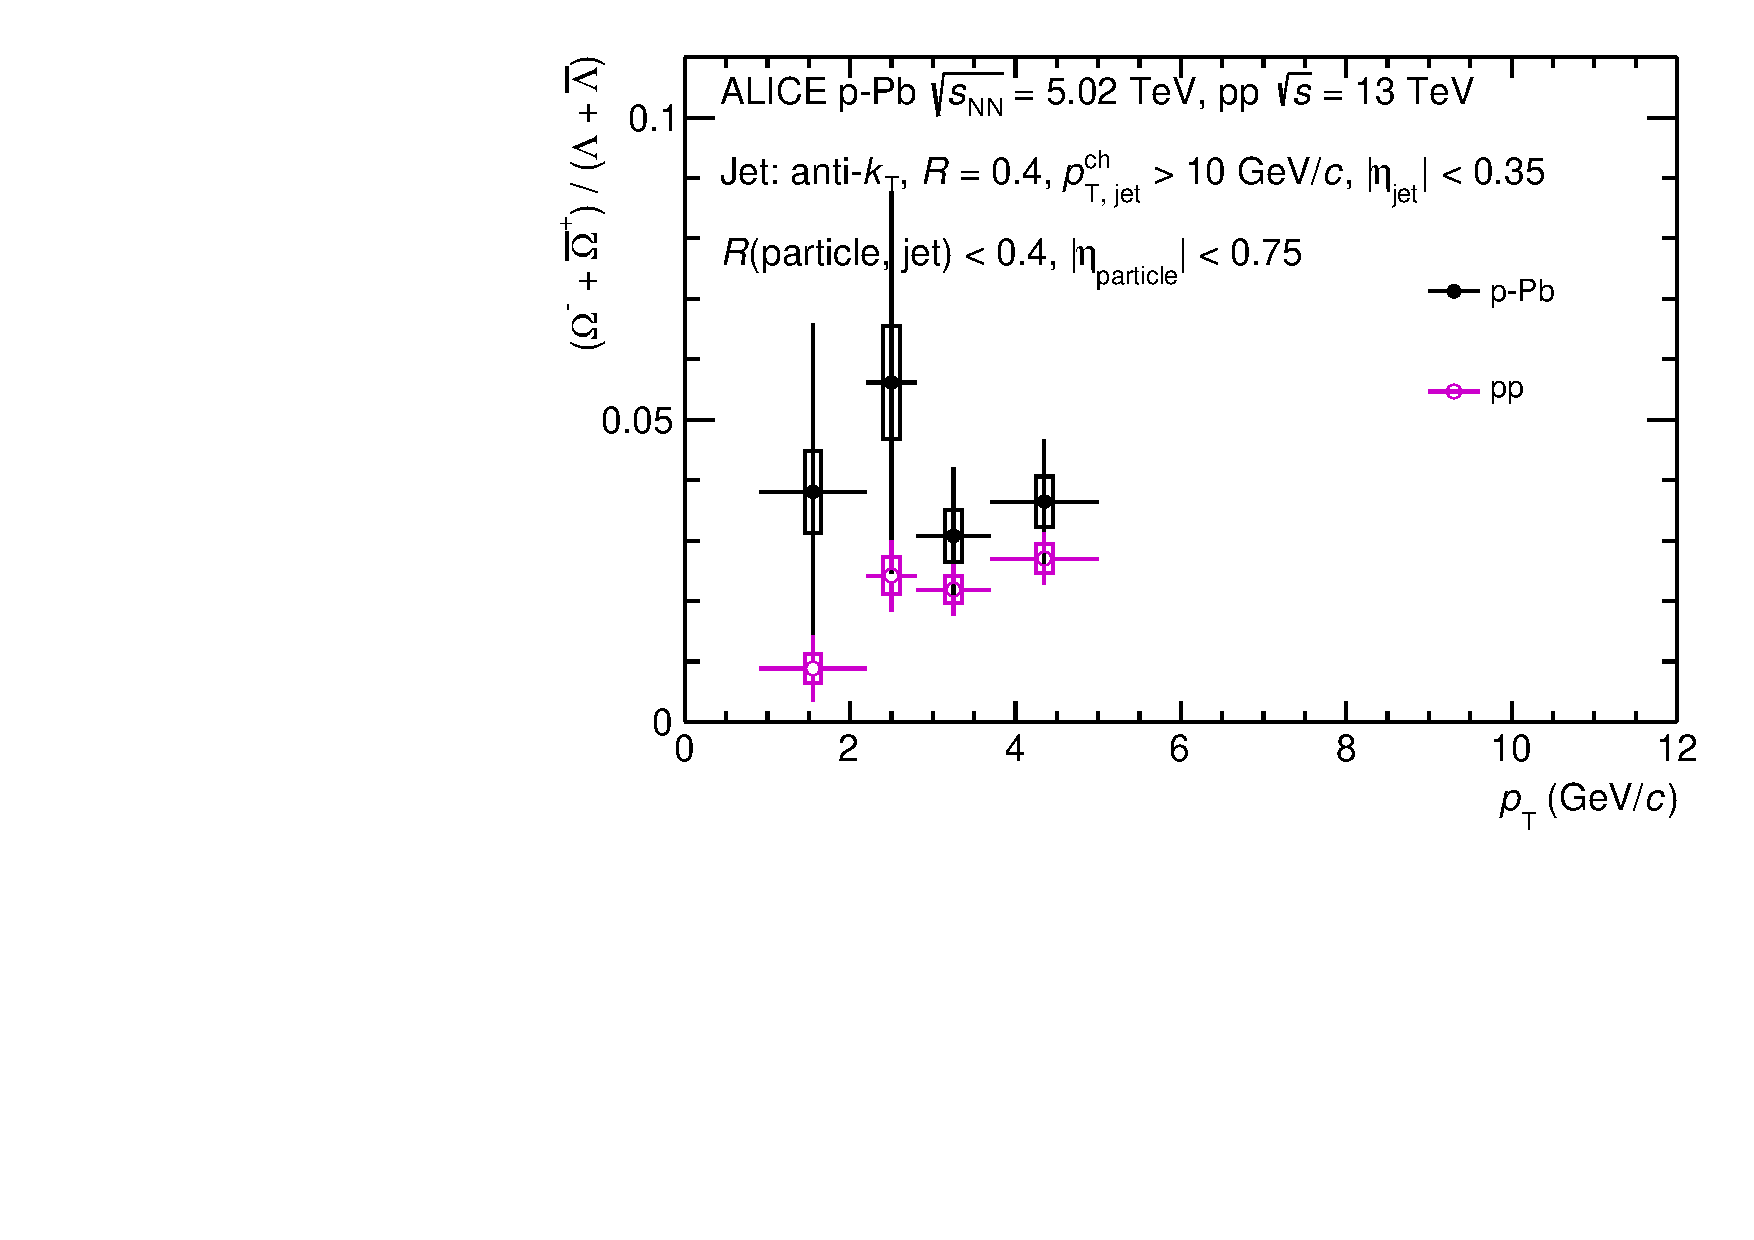
\includegraphics[width=.3\textwidth]{cf09_5}
		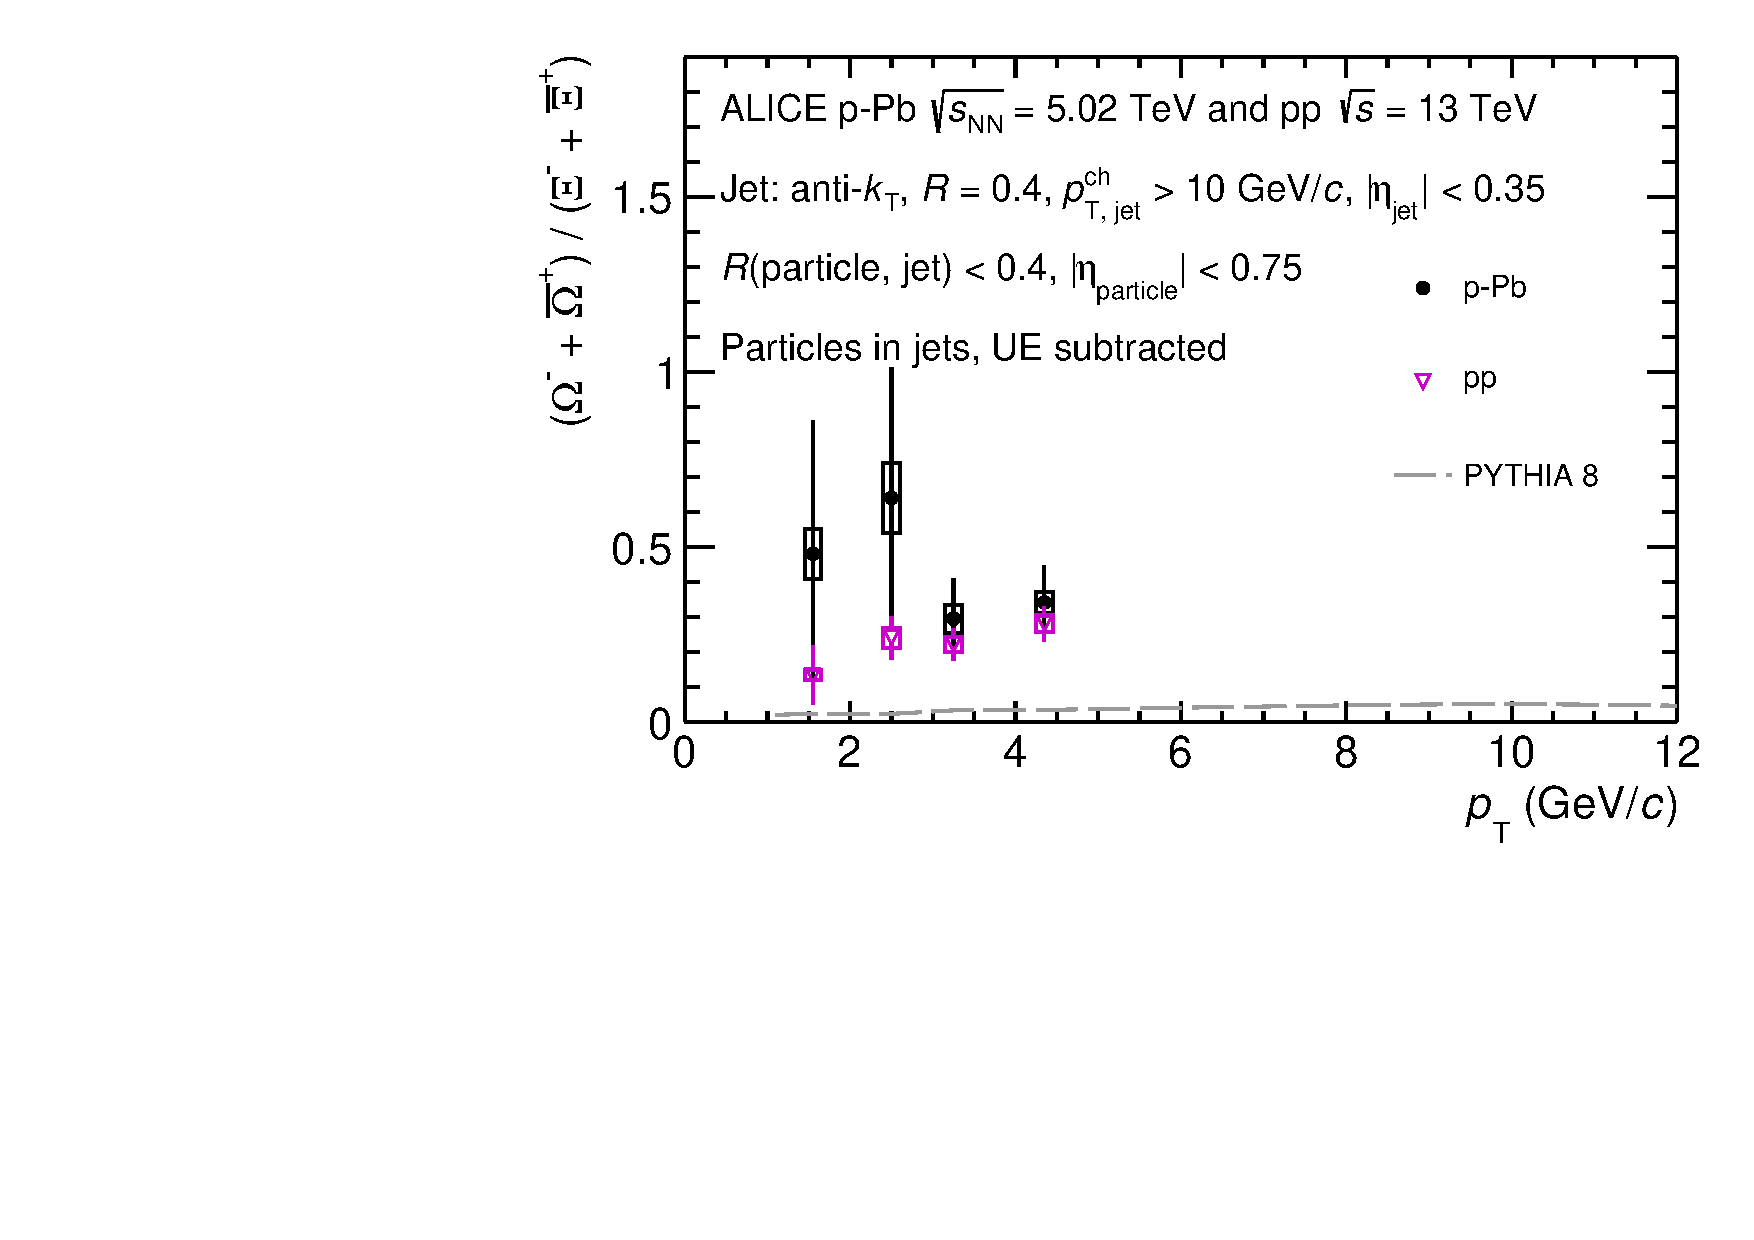
\includegraphics[width=.3\textwidth]{cf09_6}
	\end{center}
	\caption{The baryon-to-meson (top) and baryon-to-baryon(bottom) ratio as a function of particle $\pT$ in jets in \pp (open symbols) and \pPb (full symbols). The different centrality classes for \pPb collisions are depicted with different color.}
	\label{fig:pppPbRatio}
\end{figure}

\subsection{Comparison to models}
\label{subsec:ComToMod}

need to be added.

\begin{figure}[!ht]
	\begin{center}
		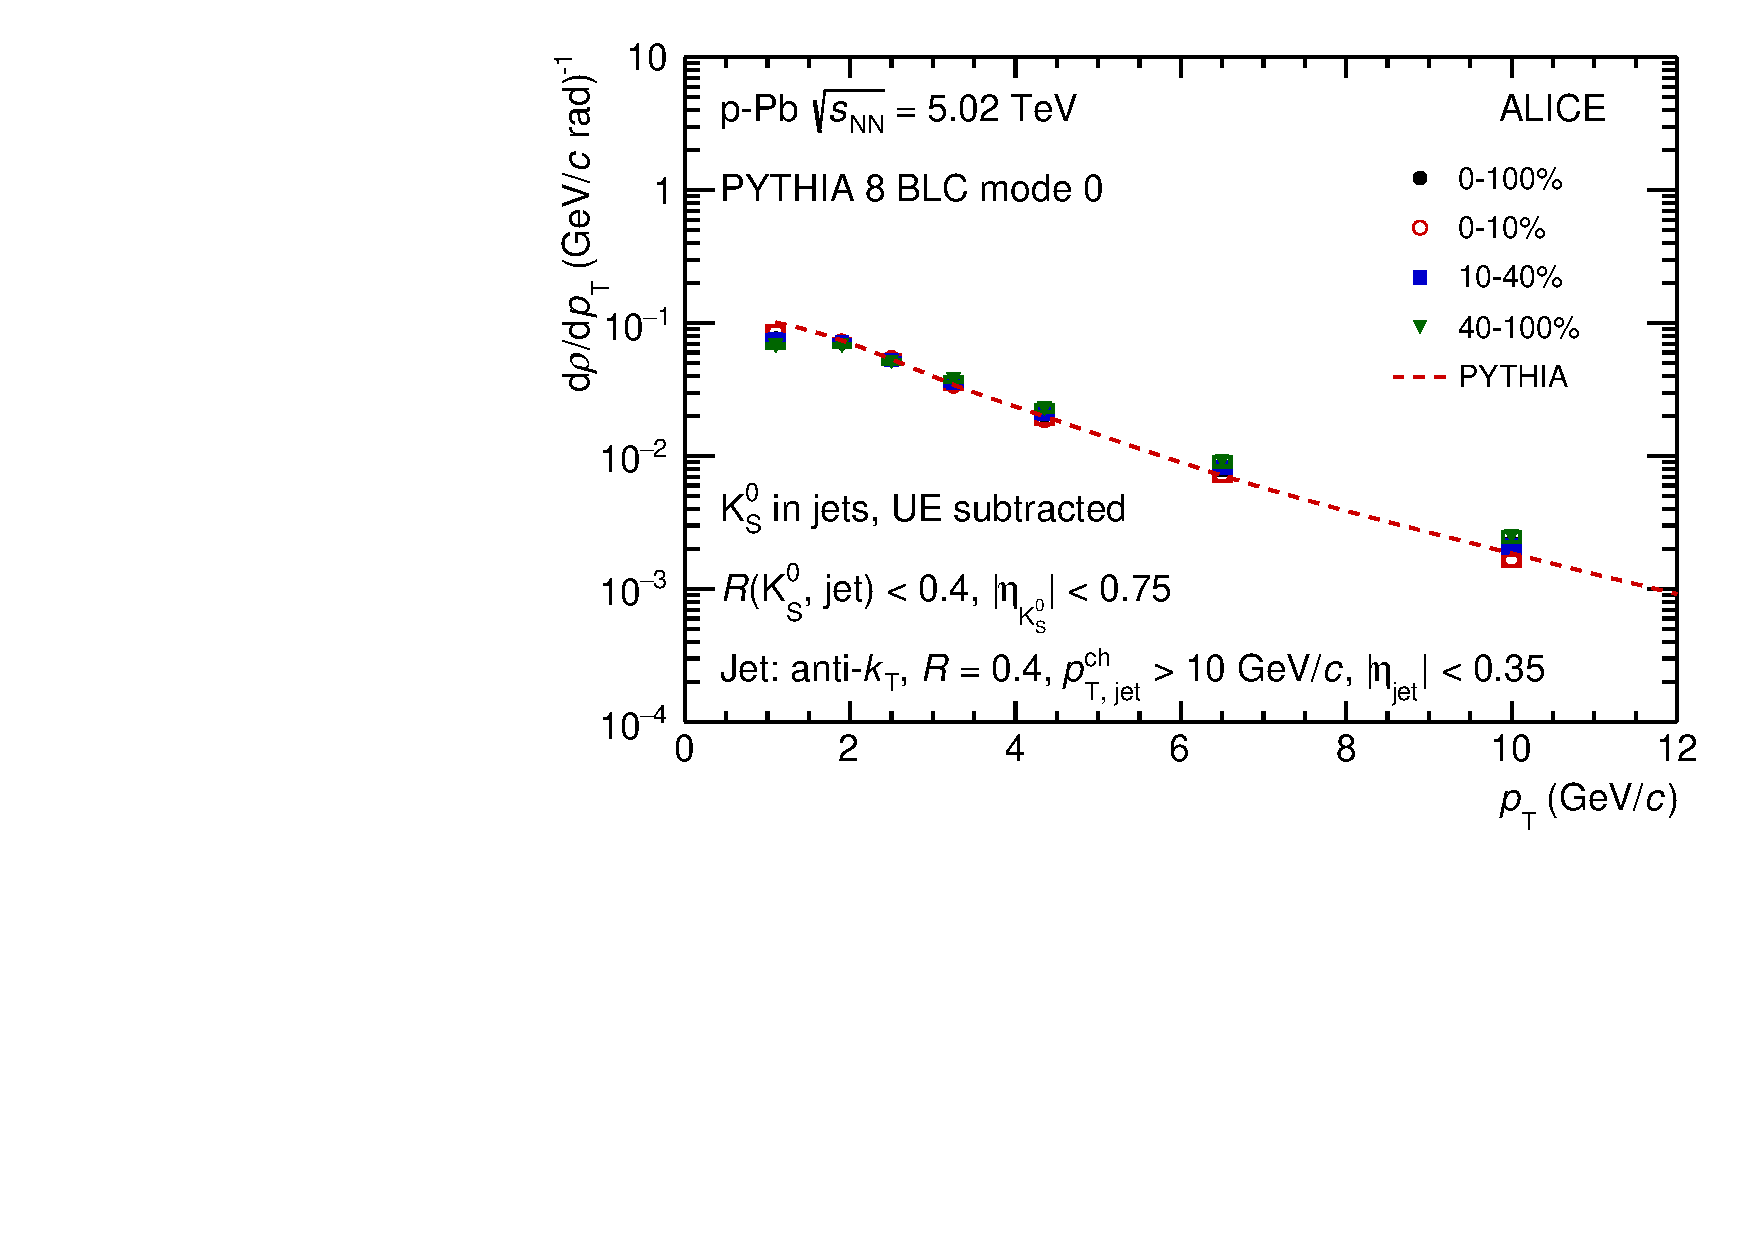
\includegraphics[width=.4\textwidth]{cf10_1}
		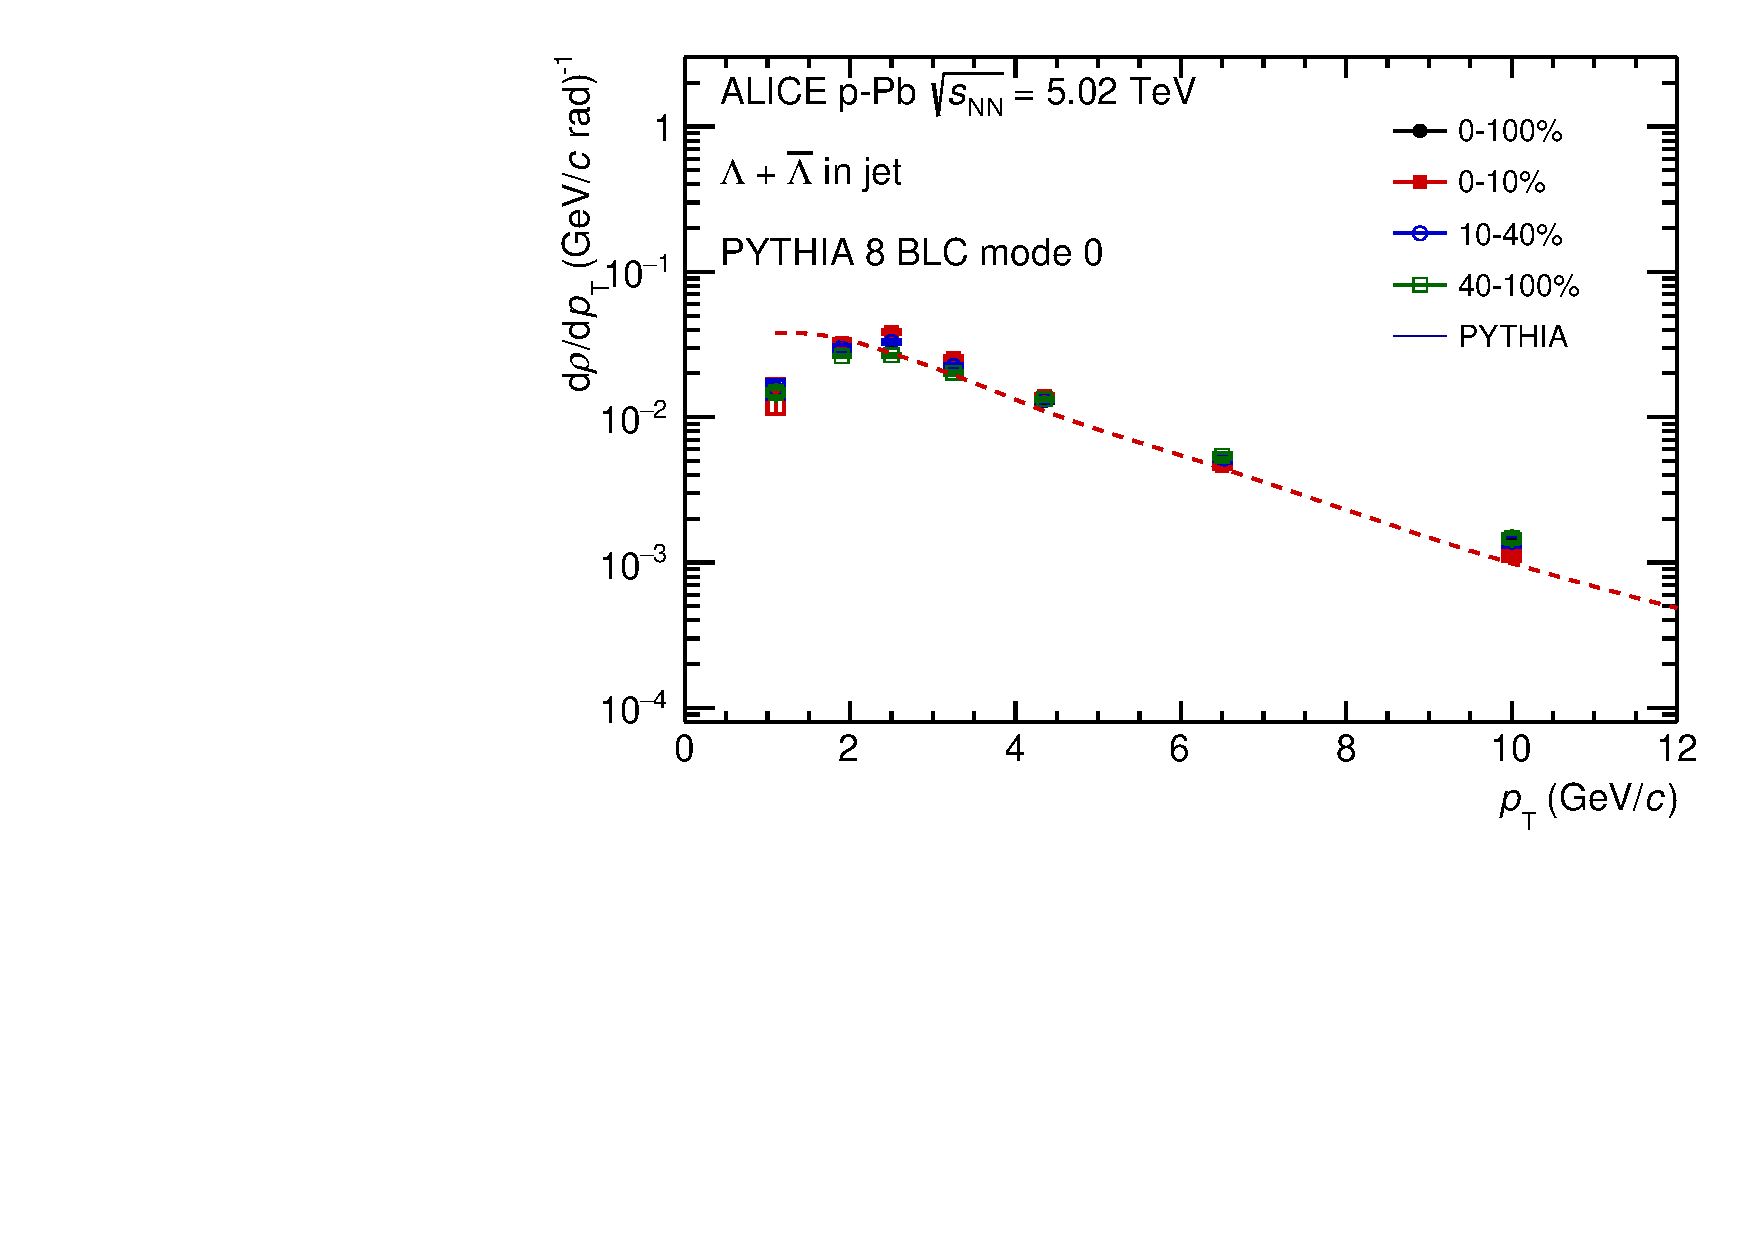
\includegraphics[width=.4\textwidth]{cf10_2}
		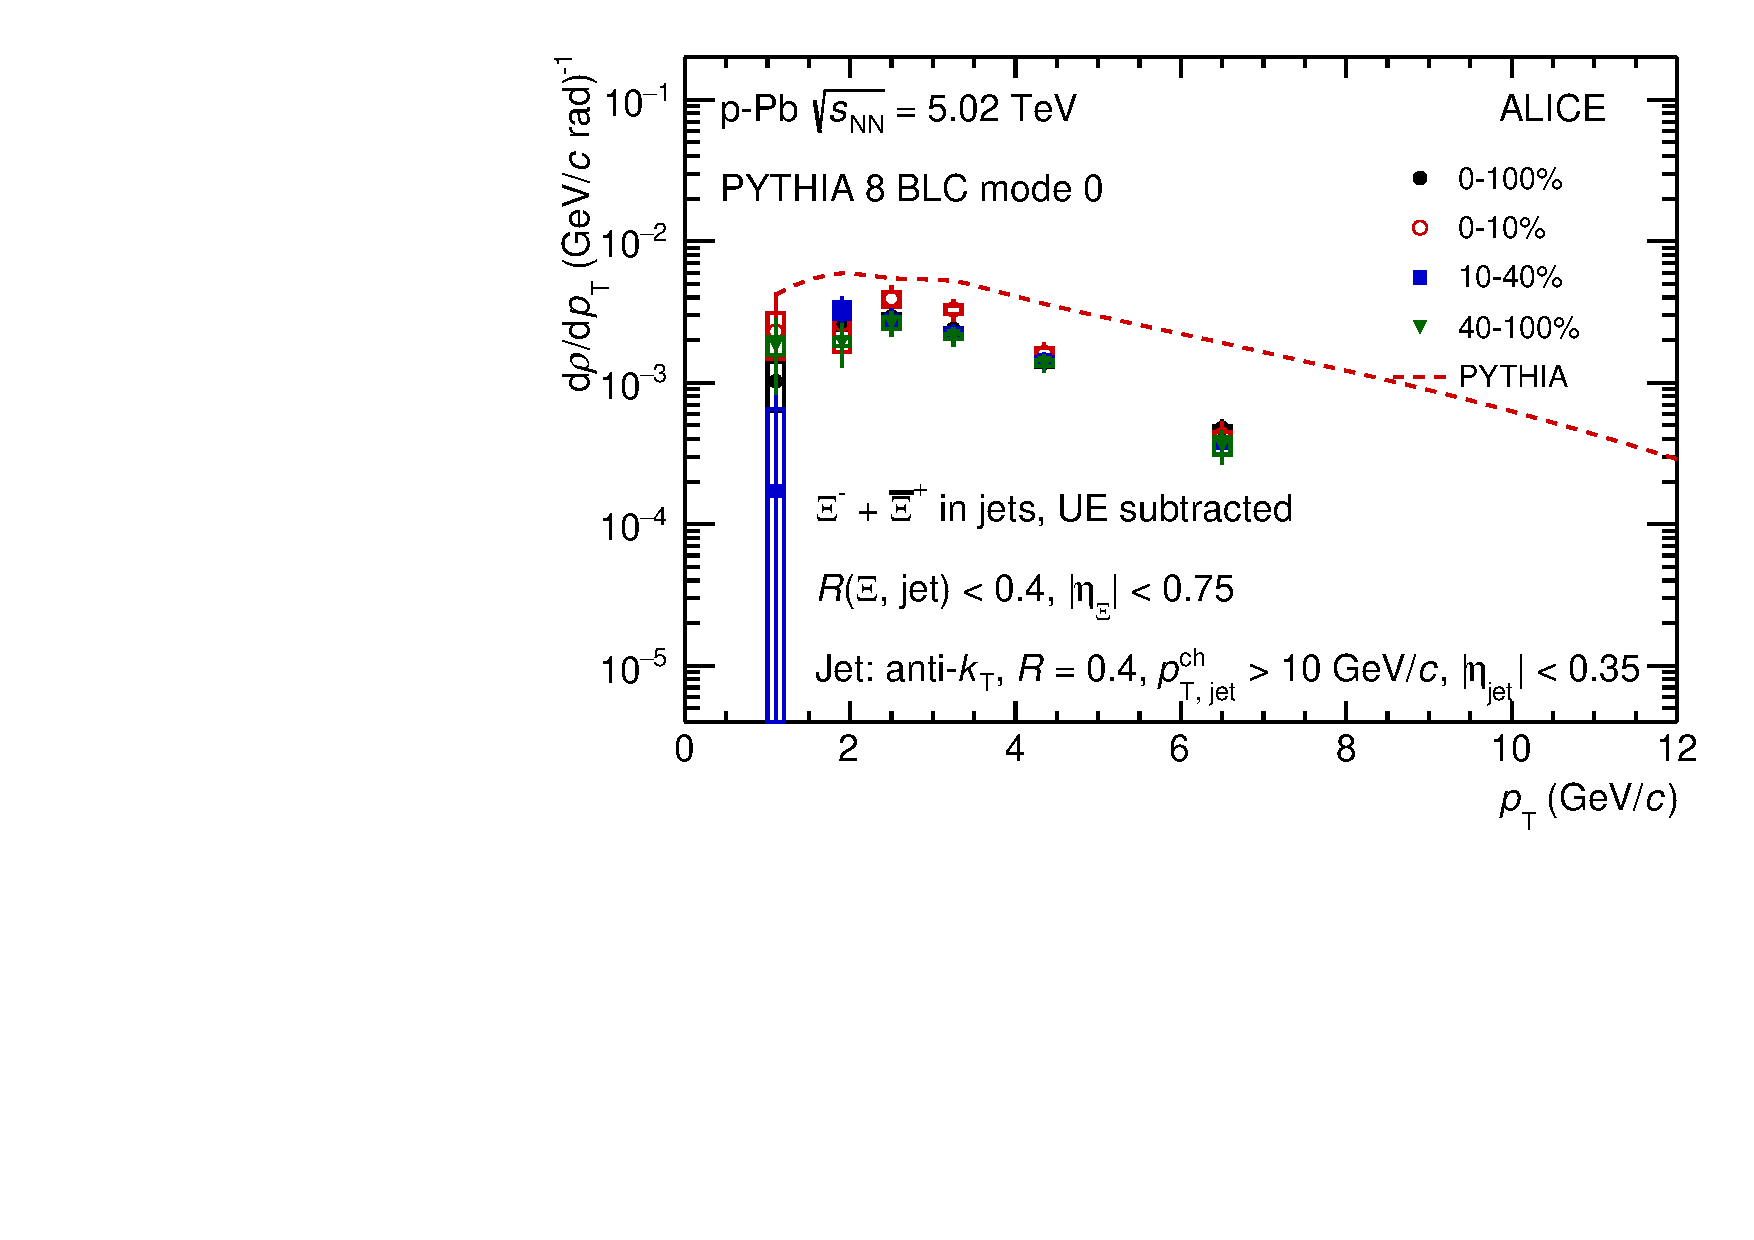
\includegraphics[width=.4\textwidth]{cf10_3}
		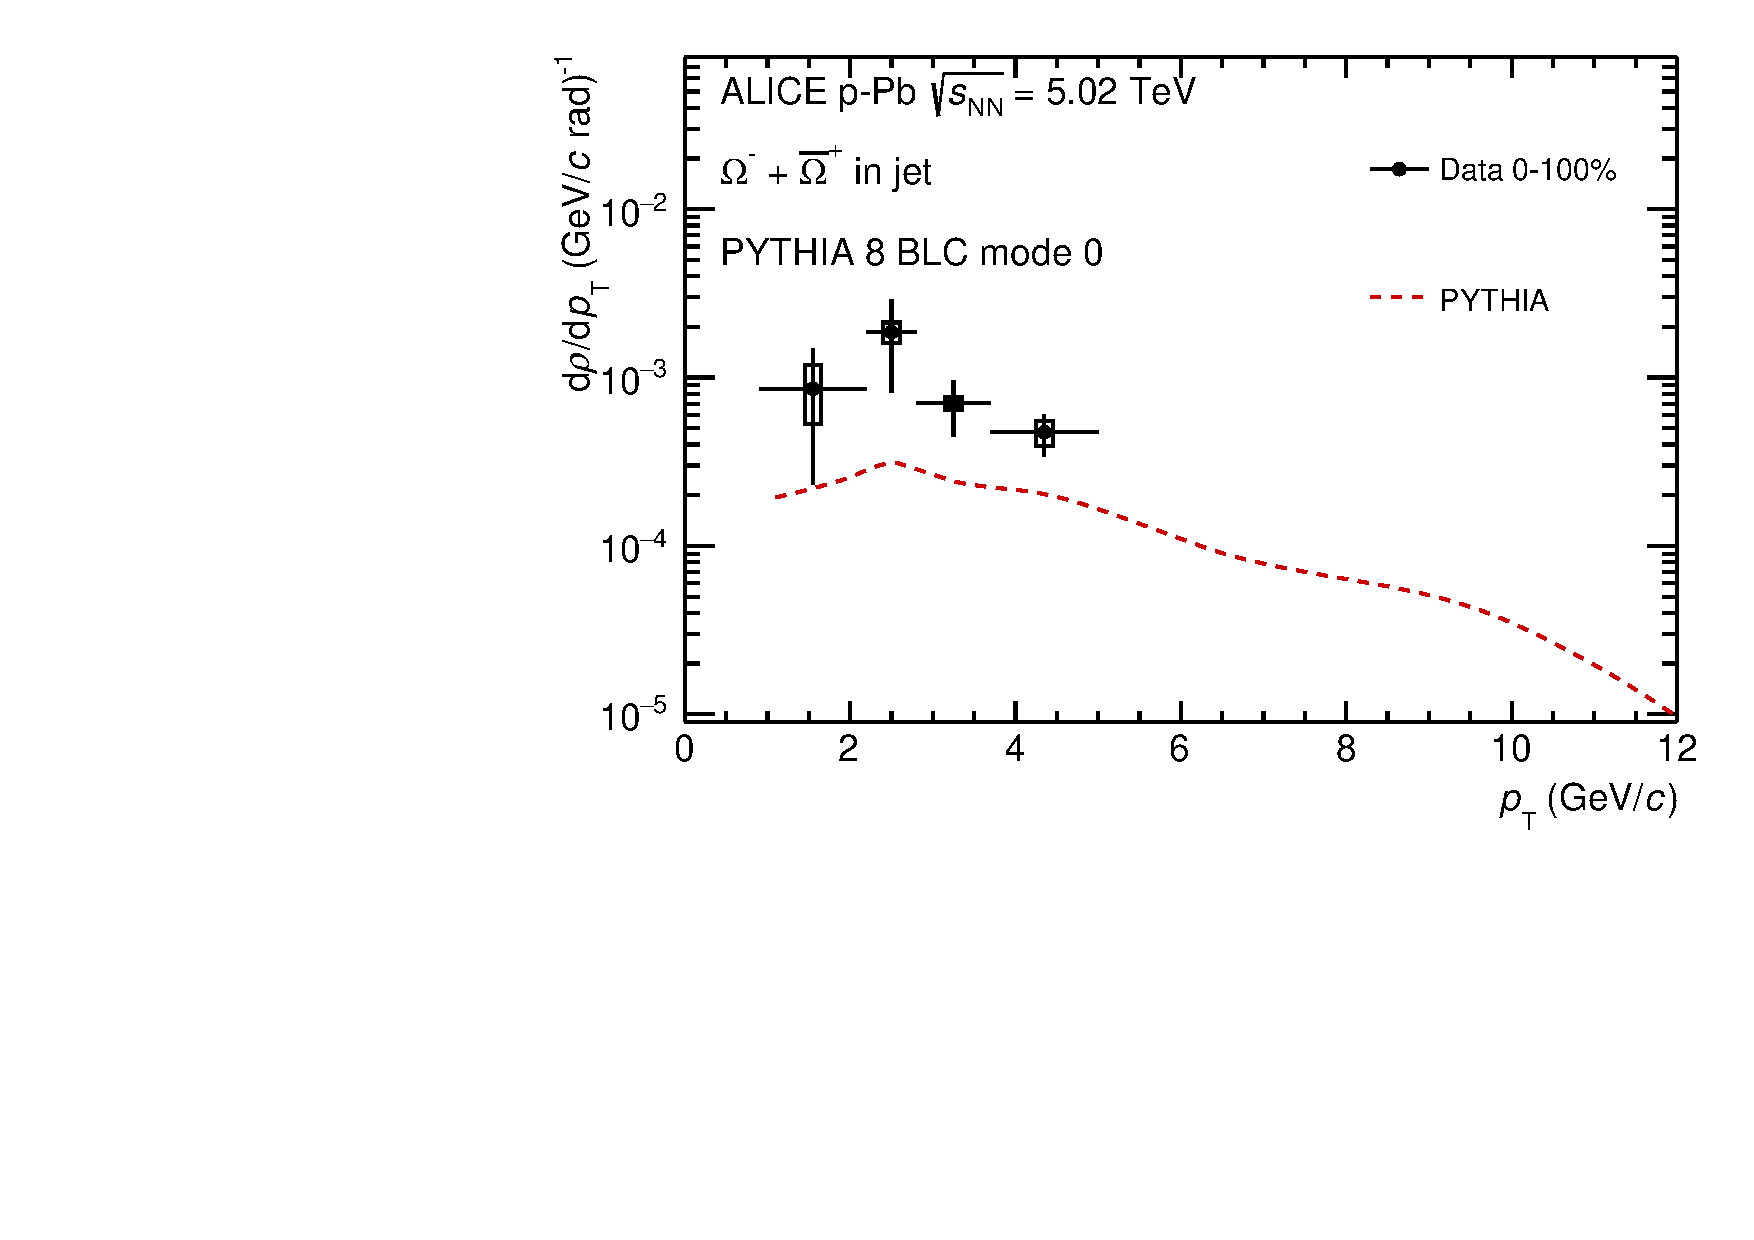
\includegraphics[width=.4\textwidth]{cf10_4}

	\end{center}
	\caption{Particles in jet in \pPb at \fivenn with PYTHIA 8 BLC mode 0}
	\label{fig:pPbpyJESpect}
\end{figure}


\clearpage
\section{Summary}%
\label{sec:Summary}

We studied the \kzero, \lmb (\almb), \Xis and \Oms $\pT$-differential density, the $\lmb/\kzero$, $\Xi/\kzero$ and $\Omega/\kzero$ baryon-to-meson ratio and the $\Xi/\lmb$, $\Omega/\lmb$ and $\Omega/\Xi$ baryon-to-baryon ratio in jets and underlying events in \pp at \thirteen and \pPb at \fivenn collisions.
The main feature of this analysis is the usage of charged particle jet to separate hard and soft progress, providing new insight into the understanding of the origin of flow-like correlations observed in small systems.

The $\pT$-differential density in events with charged-particle jet ($\pTjch$ > 10~\GeVc) are observed to become harder than that in MB events.
Also, the dependence on charged-particle multiplicity found in the inclusive particle is not present for particles generated by jet fragmentation.

The enhancement of baron-to-meson ratio at intermediate $\pT$ found in the inclusive particle in \pp and \pPb collisions are not present for particles associated with hard scattering.
\emp{to be finished}
%==========================================

\newenvironment{acknowledgement}{\relax}{\relax}
\begin{acknowledgement}
\section*{Acknowledgements}
%\input{acknowledgements.tex}

\end{acknowledgement}

\bibliographystyle{etc/utphys}
\bibliography{AliStrangeJets}

\newpage
\appendix
%\input{} % put your appendices here (if any)

\section{The ALICE Collaboration}
\label{app:collab}
%\input{authorlist-preprint.tex}  
\end{document}
